% Time-stamp: <2021-04-01 10:59:51 rlafarguette>
% LateX template 
% August 2020, Romain Lafarguette, rlafarguette@imf.org

%% ---------------------------------------------------------------------------
%% Preamble: Packages and Setup
%% ---------------------------------------------------------------------------
% Document class and font
\documentclass[11pt]{article}

% Language
\usepackage[english]{babel}

% Layout
%\usepackage[margin=1in]{geometry}
\usepackage[DIV=12]{typearea} % Page layout & margin set-up
\usepackage{setspace} % Linespread
\onehalfspacing % x 1,5 spacing

% Font and encoding
\usepackage[utf8]{inputenc} % For input
\usepackage[T1]{fontenc} % For outut
\usepackage{lmodern} % Standard LateX font
\usepackage[babel=true]{microtype}  % "Subliminal refinements towards typographical perfection"
\microtypesetup{final, tracking=true, kerning=true, spacing=true}

% Graphics
\usepackage{graphicx} % Insert graphics
\graphicspath{{../output/}} % Relative paths for graphics

% Tables
\usepackage{booktabs, rotating, multirow, pdflscape} % Tabular rules and other macros

% Floats, captions and footnotes
\usepackage{float, caption, capt-of}
\captionsetup{font=large}
\newcommand{\source}[1]{\caption*{\raggedright \small {#1} \normalsize}} % Source of a chart, left aligned


% Table of contents
\usepackage[titles]{tocloft}
\renewcommand{\cftsecleader}{\cftdotfill{\cftdotsep}} % Dot every items

% Mathematics 
\usepackage{amsmath, amsthm, amssymb, mathtools, bm} % American Mathematical Society macros 

% Subfiles and separate compilations
%\usepackage{subfiles}

% Manage authors and affiliations
\usepackage{authblk} % Properly align institutions name in the title page

% References and hyper references 
\usepackage{url} % Insert url
\usepackage{natbib} % Year-name format
\usepackage{color}  % Color package
\definecolor{darkblue}{rgb}{0,0,0.44} % Customized color for external hyper references
\definecolor{burgundy}{rgb}{0.5, 0.0, 0.13} % Customized color for internal hyper references

% Hyperlinks in pdf
\usepackage[pdftex]{thumbpdf} % Thumbnails
\usepackage[%
    bookmarks=true,   % bookmarks
    bookmarksnumbered=false,
    pdfpagemode=, % bookmark closed at the opening
    pdfstartview=FitH, % all the heigth
    pdfpagelayout=SinglePage, % perpage view
    colorlinks=true, % Coloured links
    breaklinks=true, % new line for too long links
    urlcolor= darkblue, % external links color
    citecolor=darkblue, % bibliography citations
    linkcolor=burgundy, % Internal links color
    pdfborder={0 0 0}   % No borders
    ]{hyperref} % Extensive support for hypertext in LaTeX

\hypersetup{% PDF metadata
  pdftitle = {Foreign Exchange Intervention Rule for Central Banks: A Risk-Based Framework},
  pdfauthor = {Lafarguette and Veyrune},
  pdfkeywords = {Foreign Exchange Intervention Rule for Central Banks: A Risk-Based Framework},
  pdfsubject = {Finance, Financial Economics},
  pdfcreator = {Lafarguette and Veyrune},
  pdfproducer = {Lafarguette and Veyrune},
  pdfpagemode = {UseOutlines}, % When opening pdf. UseOutlines, FullScreen, etc. 
  pdfstartview = {Fit}}

% Footnote without marker, for the title
\newcommand\blfootnote[1]{%
  \begingroup
  \renewcommand\thefootnote{}\footnote{#1}%
  \addtocounter{footnote}{-1}%
  \endgroup
}

% A few macros: environments
\newenvironment{wideitemize}{\itemize\addtolength{\itemsep}{10pt}}{\enditemize}
\newenvironment{wideenumerate}{\enumerate\addtolength{\itemsep}{10pt}}{\endenumerate}


%% ---------------------------------------------------------------------------
%% Title, authors and affiliations
%% ---------------------------------------------------------------------------
\title{\textbf{Foreign Exchange Intervention Rule for Central Banks:
A Risk-Based Framework}}

\author{Romain Lafarguette and Romain Veyrune}
%\affil{International Monetary Fund} 
\date{\today}

%% ---------------------------------------------------------------------------
%% Begin the document
%% ---------------------------------------------------------------------------
\begin{document}

\maketitle      \blfootnote{Contacts:      \url{rlafarguette@imf.org}      and
\url{rveyrune@imf.org}. Corresponding author: \url{rlafarguette@imf.org}. Both
at the Monetary and Capital Markets  Department of the International Monetary Fund.  The authors thank
Tobias Adrian, Suman Basu, Dimitris Drakopoulos, Kelly Eckhold, Chris Erceg,
Andres Gonzales, Simon Gray, Darryl King, Vladimir  Klyuev, Jorge Kriljenko,
Istvan Mak, Thomas McGregor, Stephen  Mulema, Umang Rawat,  Olga Stankova, and
Kevin  Wiseman for their  comments and  insights.  Karen  Lee provided
research assistance.  The public  data and  Python codes  to  replicate the
results of  this paper  are available  at
\url{https://romainlafarguette.github.io/software/}.}

%% ---------------------------------------------------------------------------
%% Abstract
%% ---------------------------------------------------------------------------

\begin{abstract} This paper presents a rule for foreign exchange interventions
(FXI),  designed to  preserve financial  stability in  floating exchange  rate
arrangements. The FXI rule addresses a  market failure: the absence of hedging
solution for  tail exchange rate risk  (i.e.  high volatility) in  the market.
Market impairment or  overshoot of exchange rate between  two equilibria could
generate  high volatility  and threaten  financial stability  due to  unhedged
exposures to exchange rate  risk in the economy.  The rule  uses the concept of
Value at Risk (VaR) to define FXI  triggers. While it provides to the market a
hedge against tail risk, the rule  allows the exchange rate to smoothly adjust
to new  equilibria.  In addition, the  rule is budget neutral  over the medium
term,  encourages  a prudent  risk  management  in  the  market, and  is  more
resilient to  speculative attacks than  other rules, such  as fixed-volatility
rules.  The  empirical methodology is  backtested on Banco Mexico's  FXIs data
between 2008 and 2016.\\
\end{abstract}
\bigskip

\noindent \textbf{Keywords:} Foreign Exchange Interventions, Value at Risk, GARCH 

\medskip

\noindent \textbf{JEL classification:} E58 (Central Banks and Their Policies), F31 (Foreign Exchange), G17 (Financial Forecasting and Simulations)

%% ---------------------------------------------------------------------------
%% Suppress page number on title page 
%% ---------------------------------------------------------------------------
\thispagestyle{empty} 
\newpage
\pagenumbering{arabic}


%% ---------------------------------------------------------------------------
%% Table of contents, list of figures and tables
%% ---------------------------------------------------------------------------

% \begin{NoHyper}  
% \tableofcontents
% %\addtocontents{toc}{~\hfill\textbf{Page}\par}
% \thispagestyle{empty} 

% \listoftables
% %\addtocontents{lof}{~\hfill\textbf{Page}\par}
% \thispagestyle{empty} 

% \newpage
% \listoffigures

% % \addtocontents{lot}{~\hfill\textbf{Page}\par}
% \thispagestyle{empty} 
% \end{NoHyper}  

%% ---------------------------------------------------------------------------
%% Introduction
%% ---------------------------------------------------------------------------
\newpage
\pagenumbering{arabic} % Start officially the numbering

\section{Introduction}
\label{sec:introduction}

The   2019  IMF   Annual   Report  on   Exchange   Arrangement  and   Exchange
Restrictions\footnote{Available at \url{https://www.elibrary-areaer.imf.org/Pages/Home.aspx}}
classified 66 exchange arrangements as  either floating or "free" floating. In
these arrangements,  the supply and  the demand  in the foreign  exchange (FX)
market, absent official sector FX  intervention (FXI), determines the exchange
rate. The exchange  rate risk could, then, be entirely  managed by the private
sector,  often through  the use  of derivative  instruments. The  central bank
transacts FX only to manage its FX reserves or in its role as fiscal agent for
the government.  However,  a market failure constraining  the private sector’s
ability  to manage  FX risks  may significantly  increase financial  stability
risks.   Therefore, no  central  banks, in  either  floating or  free-floating
arrangements, rule out interventions on the FX market. Even central banks with
a strong  commitment to floating  did intervene in the  FX market in  cases of
exceptional stress, such as  the COVID-19 pandemic.\footnote{See, for example,
\url{https://www.fx-markets.com/foreign-exchange/4624581/chile-launches-biggest-fx-intervention-in-20-years},
\url{https://www.wsj.com/articles/norwegian-krone-soars-amid-signs-of-central-bank-intervention-11585068173}}\\

We conceptualize  central banks' FXIs  in floating  exchange rate as  a public
good,  specifically  an  insurance,  provided by  the  public  sector  against
exchange rate tail  risks. The private sector might not  be able to completely
hedge FX risk  either because markets participants have  not internalized such
risks, or because  hedging markets are incomplete in a  given jurisdiction, or
because hedging  costs cannot  be optimally  shared among  participants. Under
such  circumstances,  public  intervention  could  be  warranted  to  preserve
financial stability.  Our  approach aligns with the  literature supporting the
idea that public intervention is desirable  when a market failure prevents the
market to supply optimally a desirable public good (\cite{stiglitz1993}).\\

Economies are  more vulnerable to large  variations in the exchange  rate when
unhedged exposures are  larger. Exposures can be  direct, such as a  firm or a
household borrows in FX while its  income is denominated in local currency, or
indirect, such  as the exchange  rate pass  through on domestic  prices, which
ultimately affects the welfare of economic agents. FX market microstructure–in
particular depth  and liquidity–plays a  role as liquid markets  absorb shocks
smoothly,   reducing  the   likelihood  of   sudden  volatility   pikes.   The
macro-financial risk materializes when a  large swing in exchange rate impacts
vulnerable agents,  leading to  balance sheets  impairments, which  could have
systemic  implications. In  other words,  vulnerable economies–with  pervasive
unhedged  exposures (e.g.   dollarized small  open economies)  and shallow  FX
markets–would  require more  public insurance  coverage against  FX volatility
compared  to  more  robust  economies  with  less  significant  exposures  and
resilient FX markets.\\

The rule proposed in this paper does  not indicate how much of the risk should
be covered  by the central  bank. Instead,  this paper designs  an operational
framework that ensures that the central bank can easily provide an FX hedge to
the market,  in a consistent  and transparent way. Public  insurance provision
entails pitfalls, such  as the cost of the insurance  and the proper alignment
of incentives  to avoid  moral hazard  reflected in  excessive risk  taking by
private agents  (\cite{mckinnon2000}).  Central  banks habitually keep  a fair
degree of opacity about their  intervention triggers, which makes it difficult
to determine how much exchange rate risk they consider the market could manage
on its own.  Often, central banks do not formally assess exposures to unhedged
exchange rate  risk in the  economy and how much  risk their FXI  are removing
from the market. Although not formalized by central banks, FXI risk mitigation
could  be inferred  ex-post  from  actual interventions  if  granular data  on
interventions are available.  Other central  banks, such as those in Colombia,
Guatemala, and Mexico, use  transparent intervention rules (\cite{chamon2019})
that partially reveal how much of the risk they intend to cover themselves.\\

In  this  paper, an  intervention  is  deemed  rule-based  when it  reacts  to
predetermined parameters to deliver predictable responses. The most frequently
used  FXI rules  are based  on  fixed-volatility triggers  such as  day-to-day
exchange rate change, for example 2 percent depreciation from the previous day
exchange rate  close. The  FXI rule  can be  disclosed or  kept secret  by the
central bank,  although, in the  latter case,  it may become  transparent with
experience. \cite{patel2019} surveyed 21 emerging market central banks and six
out  the   21  regularly  use   an  intervention   rule,  while  four   do  so
occasionally.\\

Foreign exchange intervention rules are used to anchor agents’ expectation and
influence  their behaviors  such as  to  support the  central bank  objectives
(\cite{krugman1991},   \cite{montoro2013},   and   \cite{fanelli2020}).    The
shortcoming of  many FXI rules  is that they might  not be flexible  enough to
accommodate  a  wide range  of  situations,  and  may  have to  be  abandoned,
challenging    ex   ante    the   authority’s    commitment   to    the   rule
(\cite{kydland1977}).  In this paper, we consider  the rule as an input in the
FXI  decision without  discussing  what weight  should be  given  to the  rule
compared with policy marker judgement. The  objective of paper is more to help
central bank in developing tools for FXI than to contribute to the rule versus
discretion literature (\cite{barro1983} and \cite{taylor2017}).\\

The recent  conceptual framework developed  by the IMF, the  Integrated Policy
Framework  (IPF),  provides new  theoretical  foundations  to FXIs.   The  IPF
integrates monetary  policy, exchange  rate policy, capital  flows management,
and financial stability into a unified approach (\cite{basu2020}).\\

In the IPF, deviations from the  uncovered interest rate parity (UIP) motivate
FXIs in  the spot market. Deviations  from the uncovered interest  rate parity
(the  UIP risk  premium)  signal market  dysfunctions (\cite{imf2020}),  which
arise  from  imperfect  arbitrage  by   financial  intermediaries  in  the  FX
market. UIP-deviations  based FXI would  address FX market  dysfunctions which
originate from impaired arbitrage, and not from a structural adjustment of the
real exchange  rate, which should  take place to  allow the economy  to absorb
shocks. FXIs  are expected to reduce  the UIP risk premium,  thereby improving
economic  welfare  through  a  re-alignment  of the  real  exchange  with  its
equilibrium  value. Therefore,  the IPF  presents  UIP-based FXI  as a  useful
complement to monetary policy, which could also have positive implications for
financial stability.\\

In real  time, however, it  might be operationally challenging  to distinguish
between structural shocks and UIP deviations. The estimation of UIP deviations
relies  on the  expected future  spot rate,  which might  not be  available or
accurately measured  when the  FX shock  hits the  market. The  UIP-based FXI,
while  optimal  theoretically,  cannot  always  be  implemented  in  practice,
particularly  in  markets  with  limited   depth  and  liquidity,  and  scarce
information. Still, these markets are precisely  those where FXIs are the most
needed. Therefore, a practical implementable approach is necessary.\\

This  paper  proposes an  operational  framework  based  on  a VaR  metric  to
determine the triggers of an FXI rule  (the VaR rule). Like the UIP-based FXI,
the VaR rule  allows exchange rate to reach a  new equilibrium, while reducing
the risk of exchange  rate overshot. The VaR-rule controls the  FX risk on the
market, thereby contributing  to its stability. Since the  central bank always
leave  a certain  degree of  risk on  the market,  the VaR  rule encourages  a
prudent exchange rate risk management by the private sector and stimulates the
demand  for  market-to-market  FX  hedging.    Besides,  VaR  FXI  has  unique
advantages, such as  budget neutrality over the medium-term  and robustness to
market manipulation. Finally,  the fixed frequency of FXIs under  the VaR rule
help to determine the maximum FXI  amount consistent with both (i) the reserve
adequacy constraint; and (ii) the minimum  amount necessary to have a credible
impact on the exchange rate.\\

The empirical  methodology is backtested  using Mexico data. The  Mexican peso
has floated  for a  long period  in one of  the most  liquid FX  markets among
emerging economies. In addition, Banco Mexico’s (BM) website provides detailed
intervention data since 2008. Banco Mexico also implemented interventions both
with a  minimum bid rate; that  is, a preannounced fixed-volatility  rule, and
without  a  minimum  bid  rate,   providing  a  diversity  of  experiences  in
intervention  strategies.   Our  paper  focuses  on  one  dimension  of  FXIs:
preventing  exchange  rate  tail   risks,  benchmarked  against  a  risk-based
metric. Other relevant motives may  have been factored into BM’s interventions
without a minimum rate and are outside of the scope of this paper.\\

The    rest   of    the    paper   is    organized    as   follows:    Section
\ref{sec:var-interventions}    formalizes     the    FXI     rule.     Section
\ref{sec:empirical-framework}  presents the  empirical  framework  based on  a
GARCH model.  Section \ref{sec:operational-framework} provides the operational
framework  for  central  banks  using  the  model  for  their  FXIs.   Section
\ref{sec:mexico-case}  back-tests the  model on  Mexico public  data.  Section
\ref{sec:conclusion} concludes.\\


%% ---------------------------------------------------------------------------
%% VaR Interventions and Exchange Rate Value-at-Risk
%% ---------------------------------------------------------------------------
\section{VaR Interventions and Exchange Rate at Risk}
\label{sec:var-interventions}


The exchange  rate at risk  ($ERaR$) is defined as  the percentile at  a given
threshold  $\theta$  of the  conditional  distribution  of the  exchange  rate
returns $r_t$; that  is, the Value-at-Risk (VaR). The VaR  measures how much a
financial variable  (here, FX spot)  might lose  with a given  probability and
during  a  set  period,  for example,  one  day.  Figure  \ref{fig:varconcept}
illustrates the concept.  Formally, assuming that the density $f(r_{t+1} | X_t
)$ is properly  defined over the real  line, the exchange rate at  risk is the
minimum of the set of values verifying the following condition:\\

\begin{equation*}
  \mathbb{P}\left[r_t \leq ERaR | X_t \right] = \theta
\end{equation*}

Where  $\mathbb{P}$ is  the  probability distribution  function  (PDF) of  the
density   $f(r_{t+1}|X_t)$.   

\begin{figure}
  \centering
\caption{VaR Concept}
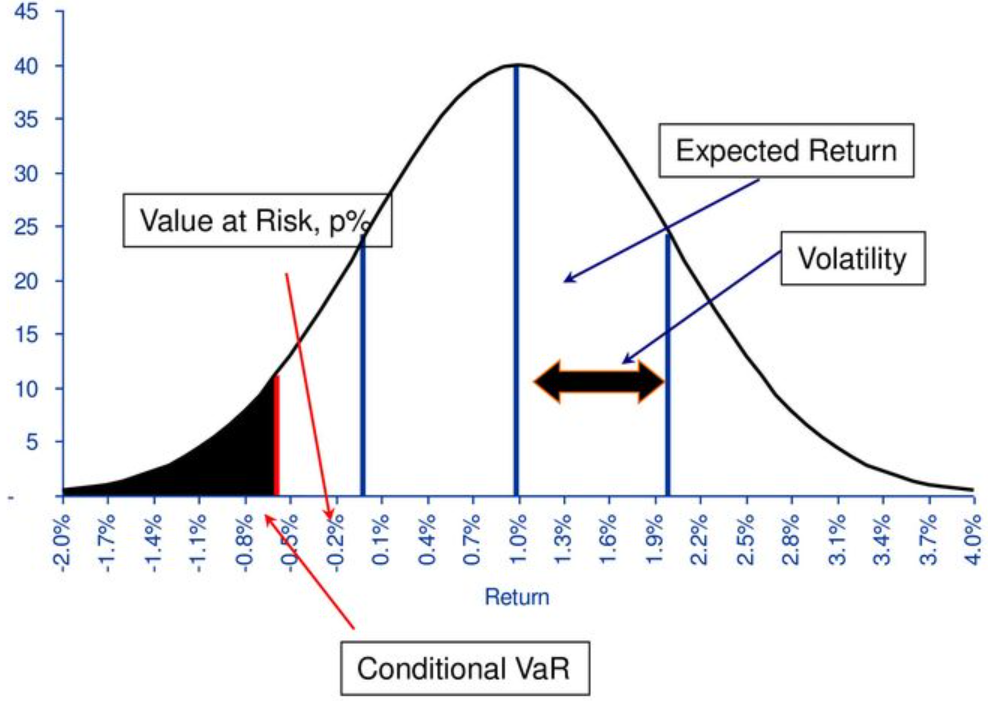
\includegraphics[width= 0.75\textwidth, keepaspectratio]{../output/varconcept.png}
\source{Source: semanticscholar.com}
\label{fig:varconcept}
\end{figure}

A conditional VaR depends on a set  of variables, which can vary in real time.
The distribution on which  the VaR is estimated is based  on the properties of
time  series  and  exogenous   regressors,  thereby  the  term  "conditional."
Following  the literature  \citep{sarno2003},  the dependent  variable is  the
log-return $r_t$ of the exchange rate $e_t$, at a daily frequency (see below).
The   conditional   predictive   density   of   exchange   rate   returns   is
$f(r_{t+1}|X_t)$ where $X_t$ is a vector of explanatory variables.

\begin{equation*}
  r_{t+1} = \log\left(\frac{e_{t+1}}{e_t}\right)
\end{equation*}


The concept of VaR, as formalized  in \cite{jorion2007}, is frequently used in
central  and  commercial banking  for  financial  applications, managing  risk
exposure,   and  portfolio   management.    \cite{alexander2009}  provides   a
comprehensive review of VaR for  market risk analysis. Among many applications
of the  VaR model,  one can  cite, in the  FX field,  \cite{aljanabi2006}, who
proposes  to  use consistently  a  VaR  framework  for managing  trading  risk
exposure  of   FX  securities  in   the  context  of  emerging   and  illiquid
markets. \cite{bredin2004} review the performance of several VaR methods using
a portfolio based on the FX exposure of a small open economy.\\


Under the VaR  approach, the policy decision determines how  much risk will be
transferred,  which has  macroeconomic  underpinning.   The quantile  $\theta$
represents the central  bank's commitment to absorb a  predetermined and fixed
share of the exchange  rate risk through its FXIs.  On  the contrary, the risk
transferred to the  central bank varies with  volatility with fixed-volatility
triggers: the  risk transfer  is high  with high volatility  and low  with low
volatility,  raising the  issue of  moral hazard  as market  participants know
ex-ante  that the  central  bank will  hedge all  volatility  above a  certain
threshold. Regarding the optimal risk transfer; i.e. the level of $\theta$, it
is a function  of the pervasiveness of exchange rate  exposures in the economy
due to currency mismatches in balance sheets and exchange rate pass-through to
domestic prices.\\


Mathematically,  the decision  rule is  formalized as  an intervention  region
$\mathcal{R}_\theta\left(r_t\right)$,   based   on   the   economy   tolerance
thresholds  for  depreciation   and  appreciation,  respectively  ($\theta_l$,
$\theta_u$).    The  decision   rule  is   binary:  if   $r_t$  falls   within
$\mathcal{R}_\theta$,  then the  central bank  intervenes; otherwise,  it does
not. These  regions evolve every day  as a function of  market conditions. In
the rest of the paper, we assume that intervention regions are symmetric, that
is,  unhedged exposures  to  the  exchange appreciation  are  as important  as
unhedged exposures  to depreciation,  to keep  the likelihood  of intervention
against   appreciation   equal   to    the   one   of   intervention   against
depreciation. Other  assumptions can be  made depending  on the nature  of the
risk.

\begin{equation*}
\mathcal{R}_\theta \left(r_t \right) = \left\{r_t \leq Q(r_t | X_{t-1},
    \theta_l) \right\} \cup \left\{r_t > Q(r_t | X_{t-1},
    \theta_u) \right\}
\end{equation*}

Where $Q(r_t |  X_{t-1}, \theta)$ is the $\theta$-quantile  of the conditional
log-returns distribution $f(r_{t+1}|X_t)$.\\

The VaR rule  provides an objectifiable approach to FXIs.  It gives the policy
maker a clear  anchor when deciding on intervention which  is directly derived
from  the financial  stability objective.  Fixed-volatility triggers  could be
derived from  an analysis of  the volatility  that the market  could tolerate;
however, they are one more step remote from the policy objective.\\

The  VaR  rule  is  financially  sound for  the  central  bank  (see  Appendix
\ref{sec:fin-perf}).   The  central bank  buys  and  sells  FX with  the  same
probability (with symmetric FXI, for instance 5\% and 95\%) at the extremes of
the exchange rate distribution, and on  the "good side" of the market (selling
expensive  and  buying  cheap),   thereby  using  its  resources  efficiently.
Profitability   has  been   associated  in   the  literature   with  efficient
intervention    to    support     FX    markets    (\cite{friedman1953}    and
\cite{sandri2020}).\\

%% ---------------------------------------------------------------------------
%% Empirical Framework
%% ---------------------------------------------------------------------------
\section{Empirical Framework}
\label{sec:empirical-framework}

\subsection{Specification}
\label{sec:specification}

We use  ARCH/GARCH (Autoregressive  Conditional Heteroskedasticity/Generalized
Autoregressive  Conditional  Heteroskedasticity)   model  for  estimating  the
forward-looking   exchange   rate   Value  at   Risk   $Q(r_t|   t-1,\theta)$.
\cite{engle2001} conducted  a comprehensive overview of  the ARCH/GARCH models
in financial econometrics in which he  devoted an entire section to estimating
VaR. \cite{giot2004} model daily VaR using realized volatility and ARCH models
and show that  it has excellent forecasting  performances. \cite{chan2007} use
nonlinear GARCH  models to estimate VaR  in the presence of  a data generating
process with heavy tails.\\

Other  types  of models  could  be  used to  estimate  VaR,  such as  quantile
regressions   (\cite{gaglianone2011}),    copulas   (\cite{patton2001}),   and
nonparametric kernel  (\cite{hoogerheide2010}).  However,  the GARCH  model is
used in this paper because it is  commonly used in the industry and by central
banks. GARCH models  relies on standard maximum likelihood  estimators and are
implemented    in   many    statistical   packages,    making   them    easily
operationalizable.   Besides, as  \cite{jeon2002} show,  FX markets  are quite
efficient,  and their  features fit  well the  simple and  robust approach  of
standard  GARCH models.   Finally, GARCH  models are  frequently used  for the
analysis of  the FX markets.  \cite{hansen2005}  argue that in the  context of
daily exchange rate returns, no alternative model can beat a GARCH(1,1) model,
while  \cite{mcmillan2012} show  that an  intraday GARCH(1,1)  model generally
provides superior forecasts compared with all other models.\\

More precisely, the VaR rule presented here uses an Exponential GARCH (EGARCH)
model  of volatility.   The advantage  of the  EGARCH model  is that  it is  a
relatively   parsimonious   model   which  incorporates   nonlinearities   and
asymmetries with only  two equations. Exceeding a certain  level of volatility
could result  in sudden shifts  in expectations, closing large  positions, and
herding behavior  among market  participants. Besides,  markets may  not react
equally to exchange rate appreciation and depreciation. The model presented is
a  proof   of  concept  and  could   be  refined  by  the   central  bank  for
implementation.\\

The EGARCH specification incorporates three components: drift, volatility, and
the distribution of the error terms or innovations.\\

\begin{itemize}
\item \textbf{Drift}: $r_t= \bm{Intercept} + \bm{\rho} r_{t-1} + \bm{\beta}
X_t + \varepsilon_t$ AR-X(p) for the average level of log-returns ($r_t$, the
drift), and  $X_t$ a vector of  exogenous regressors.  The drift  reflects the
conditional exchange rate trend

\item \textbf{Volatility}: $\log \sigma_t^2 = \bm{\omega} + \bm{\beta} g(r_{t-1}) \text{with} \
  g(r_t)= \bm{\alpha} r_t + \bm{\gamma}(|r_t| - \mathbb{E}[|r_t|])$: where $\sigma_t$  is
  the volatility 

\item \textbf{Errors term}: $\varepsilon_t = \sigma_t \epsilon_t,\ \epsilon_t \sim TSK\
(\bm{\nu}, \bm{\lambda})$: the error term is parameterized for instance with
a Tskew  distribution (other  distributions can be  used, including  Normal, T
distribution and generalized error distributions).
  
\end{itemize}

The parameters in \textbf{bold} are estimated by the GARCH model.\\

The  estimates  use  an  EGARCH-X(1,1)  with  Tskew  distributed  innovations,
estimated  via  Maximum  Likelihood  Estimation.\footnote{We  built  a  Python
wrapper around  the comprehensive  "ARCH" Python  package, developed  by Kevin
Sheppard  from Oxford  University  \citep{sheppard2020}} GARCH  models are  a
standard approach to estimating  and forecasting volatility \citep{engle2001}.
The number  and order  of lags  are chosen based  on AIC/BIC  criteria (Akaike
Information Criterion/Bayesian  Information Criterion).  An  alternative model
is  the  JP  Morgan  RiskMetrics model  \citep{zumbach2007},  with  exogeneous
regressors and  innovations distributed  with generalized  error distribution,
also   known    as   generalized    Gaussian   distribution    (GGD).    Annex
\ref{sec:benchmarking}  presents  different   specifications  and  alternative
models as a robustness exercise.\\

With  the GARCH  specification  presented above,  the VaR  rule  allows for  a
progressive adjustment of the exchange rate  to its new equilibrium value. The
estimated conditional volatility  includes a drift that  reflects the exchange
rate trend and reduces the likelihood that the VaR rule triggers FXIs when the
exchange rate  is on an appreciating  or depreciating trend. In  addition, the
conditional  distribution  changes with  the  volatility  regime to  keep  the
likelihood  of  interventions unchanged,  thereby  loosening  the triggers  as
volatility increases.  On the contrary, fixed-volatility rules do not adapt to
trends and volatility regimes.\\

The exchange rate adjustment to a  new equilibrium, even though necessary from
a macroeconomic  point of view, could  be disruptive because of  its impact on
expectations and market functioning. Therefore,  interventions in the tails of
the volatility distribution during the  adjustment process contribute to avoid
that the exchange rate significantly overshoots its equilibrium level, harming
financial stability.\\

The EGARCH  includes several  exogenous regressors  (EGARCH-X) to  improve the
accuracy of the conditional volatility forecast. These exogenous variables can
be  used to  factor in  the  specifics of  a  given market  and customize  the
interventions  metrics. Although  our estimation  is based  on daily  data, we
incorporated some  proxies for  intraday volatility  and liquidity  too, hence
capturing microstructure dimensions. Therefore, the VaR rule provides a single
input for the intervention decision based on multiple variables (i.e., sources
of information) that is more  straightforward to interpret than large “traffic
lights”  dashboards, where  sub-indicators might  conflict. Our  specification
includes the following regressors:

\begin{itemize}
\item \textbf{The average exchange rate bid-ask spread over the day}, taken in
  absolute terms. The finance literature uses the bid-ask spread as a proxy of
  intraday market liquidity
\item \textbf{The intraday spread (max–min over the day)}, which is another
  metric of intraday volatility
\item \textbf{The daily  interest rate differential between  local and foreign
currencies} captures  the interest  rate parity arbitrage.  We used  the daily
interest rate  differential instead of  the cross-currency basis swap,  as the
former has a longer available time series
\item \textbf{The  one-month forward  exchange rate},  expressed as  the first
difference from the day before. As the previous variable controls for interest
rate parity, the forward rate could capture  the impact of the cost of hedging
on the spot market
\item \textbf{The first-difference variation of the Chicago Board Options Exchange Volatility Index (VIX)}, which captures
  global risk sentiment\footnote{We tried with the VIX in level, but the p-value was higher than in the first difference}
\item \textbf{The exchange rate of the US dollar vis-à-vis the euro}, to
  control for US dollar specific developments
\item \textbf{Oil prices log returns}, as Mexico is an oil exporter and oil prices could impact term of trade (i.e. competitive shock)
\end{itemize}

The  VaR  rule  is  robust  to speculative  attacks  because  the  conditional
distribution   is  forecasted   by   the  EGARCH-X   model   and  updated   in
real-time.  Forward-looking variables  reduce  the risk  of opportunistic  and
strategic behaviors  from market participants. Indeed,  as market participants
are changing behavior, the VaR rule is changing too. The adaptative feature of
the  VaR  rule makes  it  more  complicated  and  even impossible  for  market
participants  to  take  speculative  positions  because  they  would  need  to
anticipate perfectly  how their new behavior,  as well as the  behavior of all
other  market participants,  will shift  the conditional  distribution of  the
exchange rate.  On the  contrary, with  fixed thresholds,  market participants
know exactly  when the central  bank will  intervene and can  take speculative
positions accordingly.\\

\subsection{Estimation Results}
\label{sec:estimation-results}

As a proof of concept, the model is  fitted against a real sample of Mexico FX
data (against  the US  dollar) since  2001. The peso  has been  floating since
1994.   Figure  \ref{fig:descriptive-plot}   presents  the  historical  level,
returns,  and  returns distribution  of  exchange  rate.  The  bilateral  spot
exchange rate  exhibits significant  volatility in crisis  times, such  as the
global financial crisis of 2008 and, more recently, the COVID-19 pandemic. The
historical  distribution  shows that  the  returns  are  skewed to  the  right
(depreciation). The model thus  incorporates asymmetries to accurately capture
the dynamics of this exchange rate  series. Intervention data are available on
the                                                                       BM's
website.\footnote{\url{https://www.banxico.org.mx/mercados/subastas-cambio-credito-banco.html}}\\

\begin{figure}
  \centering
  \caption{Mexican Peso against US Dollar}
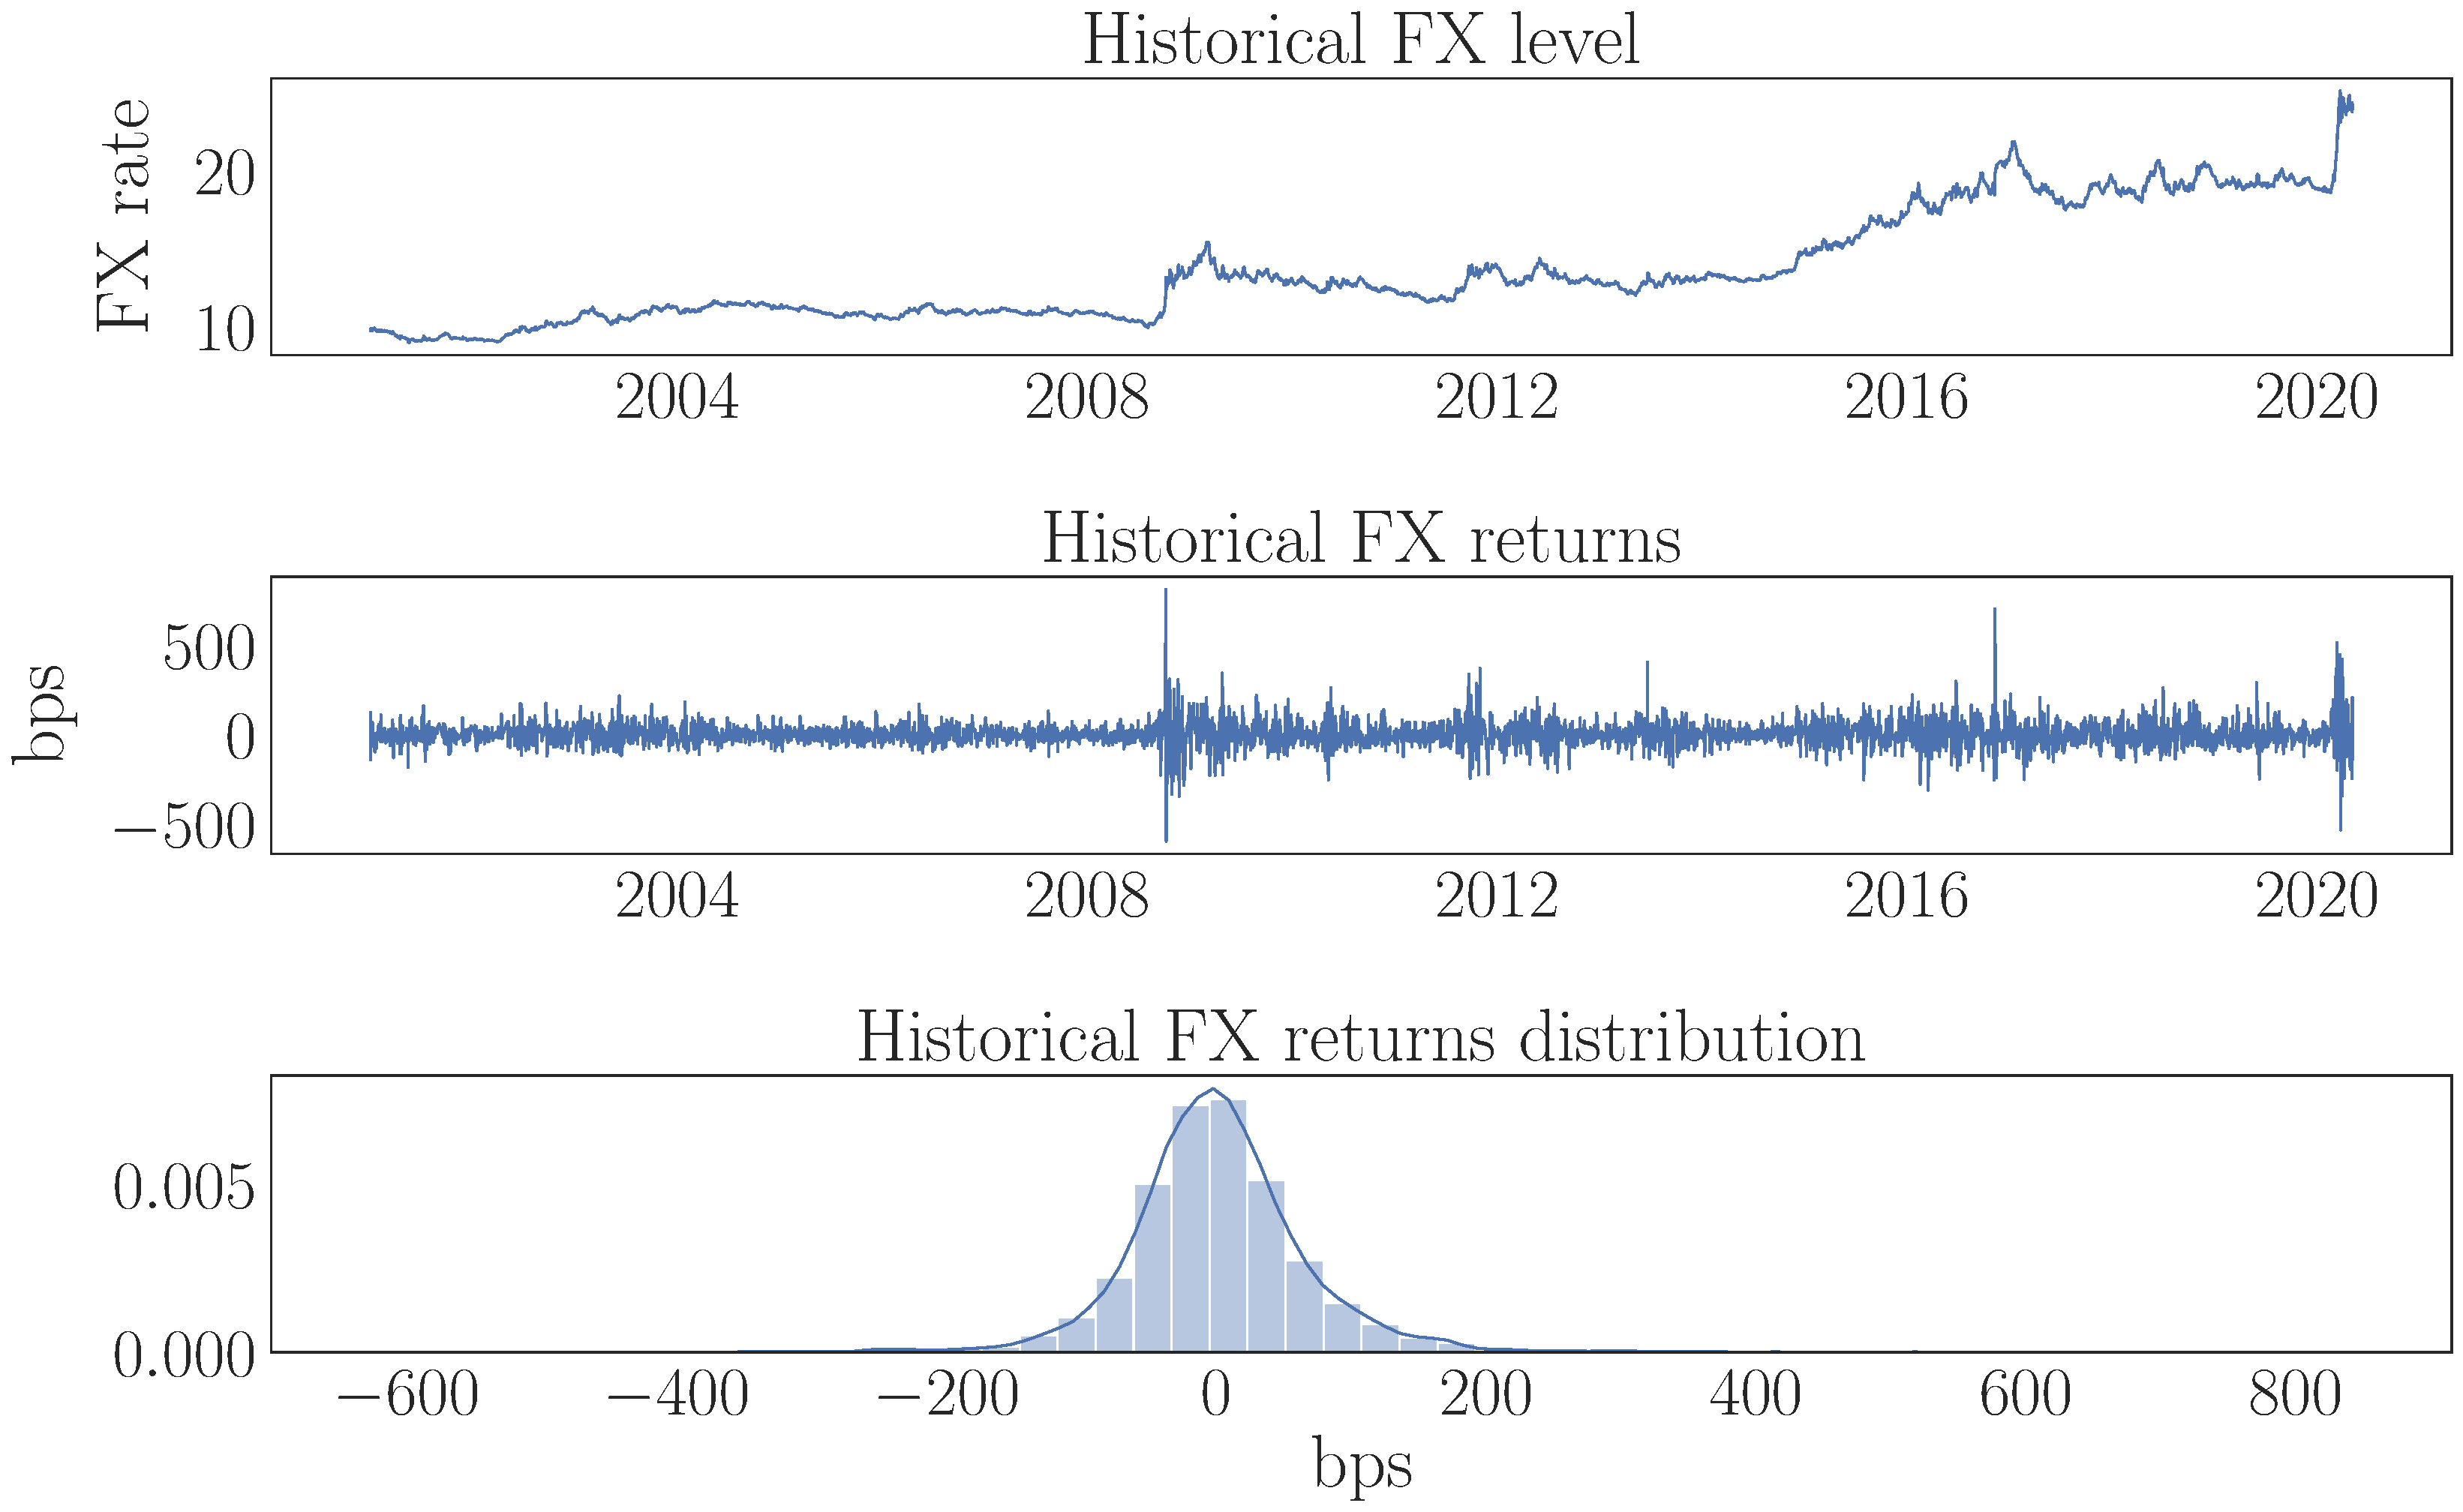
\includegraphics[width= 0.95\textwidth, keepaspectratio]{../output/descriptive_plot.pdf}
\label{fig:descriptive-plot}
\source{\emph{Sources}: Bloomberg and authors' calculations}
\end{figure}


The signs  of the coefficients  are consistent with macroeconomic  and finance
theory   (see   \cite{sarno2003}   for   an  exposition   of   exchange   rate
economics).  Table  \ref{tab:reg-coeffs}  presents  the output  of  the  GARCH
estimation process,  where we  integrate progressively the  coefficients under
different specifications,  starting from  the micro to  the macro  factors. We
have tried to  insert year dummies to control for  structural breaks, but most
of the coefficients were not significant.\\

\begin{itemize}
\item The bid-ask spread is positively correlated, suggesting that an increase
  in the bid-ask spread (market illiquidity) signals depreciation
  
\item Forward points also contribute to predicting the movement in exchange
  rate log returns, with the same sign as expected
  
\item A positive interest rate differential with the London Interbank Offered
  Rate (LIBOR) tends to appreciate the currency, due to carry-trade arbitrage
  
\item The same results hold for the VIX, as an
  increase in global risk sentiment tends to depreciate emerging market
  currencies

\item Changes in  the EUR/USD exchange rate have the  expected impact on local
currency returns and contribute to the explanatory power of the model
  
\item Similarly, with the oil price log  returns, an increase in oil prices is
associated with an appreciation of the local currency against the USD

  
\item The model explains around 28 percent of the log-return variance
\end{itemize}

\begin{table}
  \begin{center}
    \caption{Results of the GARCH Estimates} %\footnotesize
    %% command to change the font size
    \begin{tabular}{llllll}
\toprule
{} & Microstructure &       CIP & Dollar move & Risk Appetite &  Baseline \\
\midrule
Intercept                       &       -2.33*** &     -2.29 &       -1.84 &         -2.55 &     -1.63 \\
Lag FX log returns              &       -0.07*** &     -0.08 &    -0.08*** &      -0.08*** &  -0.08*** \\
Bid ask abs                     &           5.71 &     24.39 &      -35.66 &         -2.42 &      3.23 \\
Min max abs                     &       35.56*** &     34.63 &       34.32 &        34.55* &     26.21 \\
Forward points first difference &       23.29*** &  17.79*** &    26.44*** &       19.8*** &  19.44*** \\
Interbank rate vs Libor         &                &  33.61*** &    39.32*** &      34.75*** &  33.86*** \\
EURUSD log returns              &                &           &    -0.14*** &      -0.17*** &  -0.16*** \\
VIX first diff                  &                &           &             &      15.66*** &  15.37*** \\
FX intervention dummy lag       &                &           &             &               &      2.23 \\
Oil prices log returns          &                &           &             &               &  -0.02*** \\
Omega                           &        0.13*** &      0.13 &     0.12*** &       0.11*** &   0.12*** \\
Alpha                           &        0.17*** &     0.17* &     0.16*** &       0.16*** &   0.15*** \\
Gamma                           &        0.07*** &   0.06*** &     0.06*** &       0.05*** &   0.05*** \\
Beta                            &        0.98*** &   0.99*** &     0.99*** &       0.99*** &   0.99*** \\
Nu                              &        8.33*** &   8.66*** &     8.92*** &       8.71*** &   8.54*** \\
Lambda                          &        0.08*** &      0.07 &        0.09 &         0.07* &   0.08*** \\
R2                              &          5.8 \% &     6.7 \% &      10.4 \% &        27.3 \% &    27.6 \% \\
R2 adjusted                     &          5.8 \% &     6.6 \% &      10.4 \% &        27.2 \% &    27.5 \% \\
Number of observations          &           5986 &      5986 &        5682 &          5682 &      5680 \\
Significance *10\%, **5\%, ***1\%  &                &           &             &               &           \\
\bottomrule
\end{tabular}

%\normalsize \source{\emph{Sources}: authors’ calculations}
\label{tab:reg-coeffs}
\end{center}
\end{table}

Once  fitted,  the  GARCH  model  provides  an  in-sample  estimation  of  the
conditional  volatility,   $\sigma_t^2$,  over   time,  presented   in  Figure
\ref{fig:conditional-vol}.   Not   surprisingly,  the   in-sample  conditional
volatility  spikes  during  the  global  financial  crisis  and  the  COVID-19
crisis.\\

\begin{figure} \centering
  \caption{Conditional  FX   Volatility  over   Time}  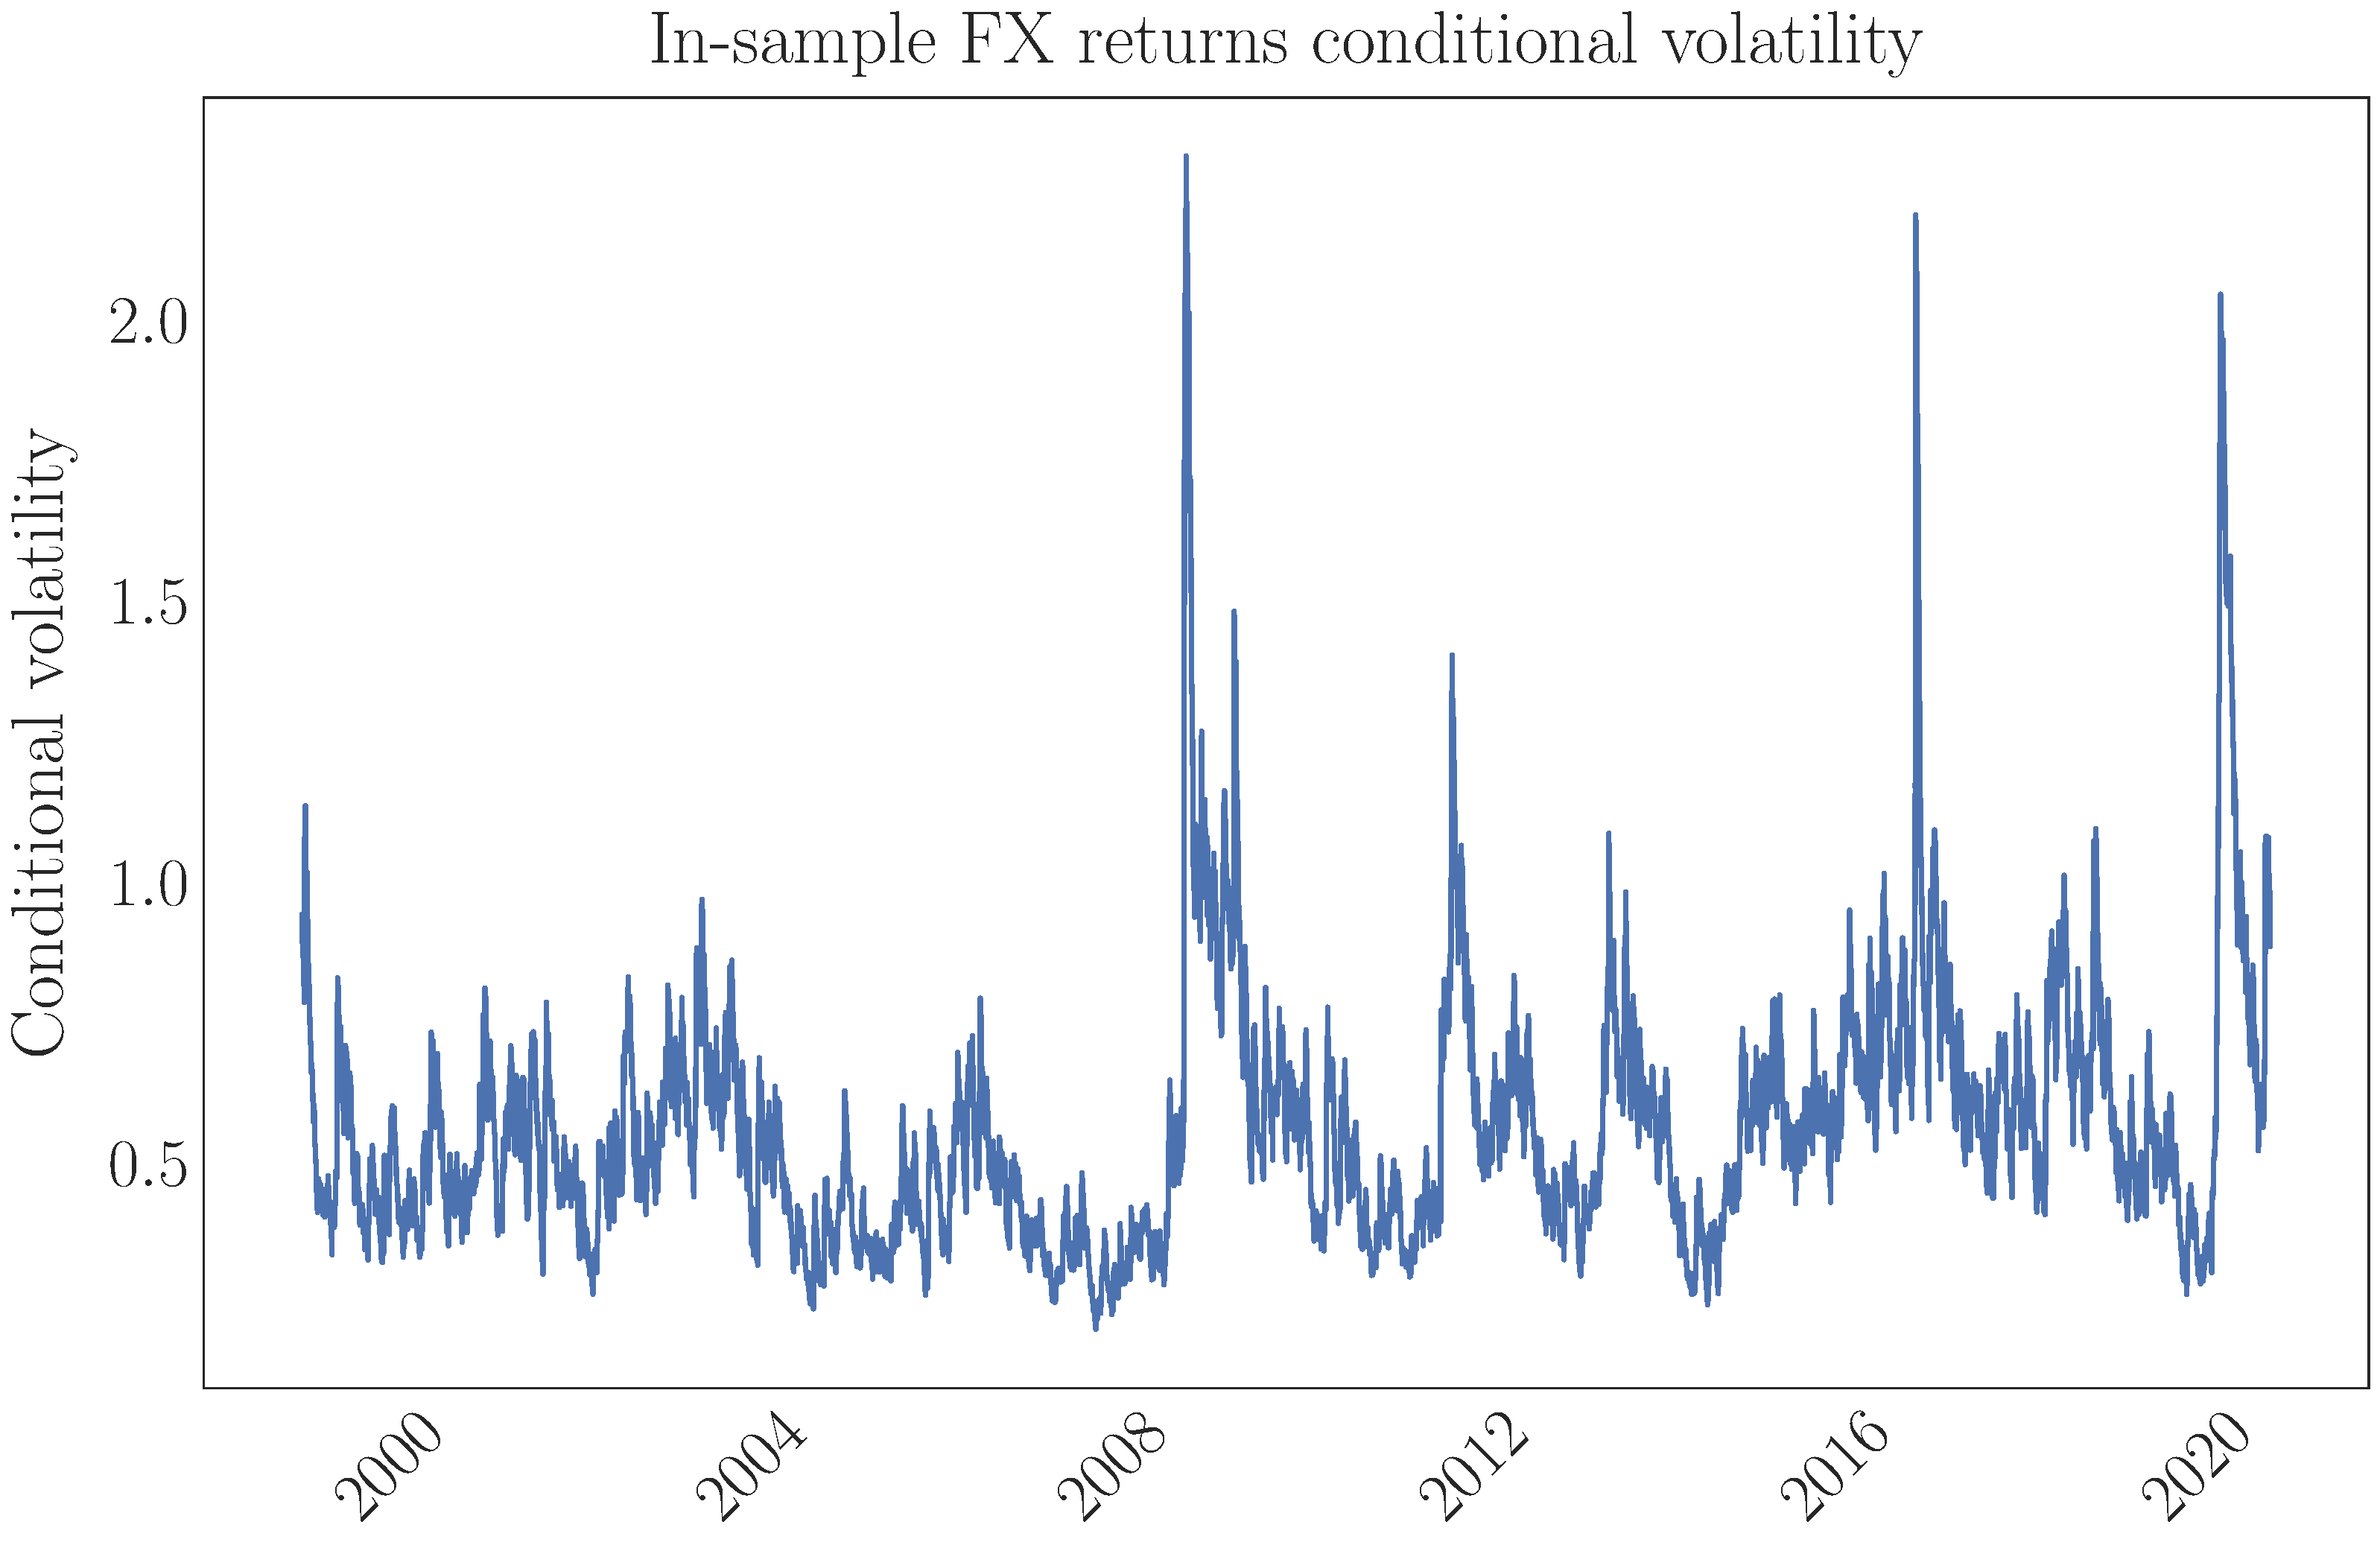
\includegraphics[width=
0.95\textwidth, keepaspectratio]{../output/conditional_vol_plot.pdf}
\label{fig:conditional-vol} \source{\emph{Sources}: authors' calculations}
\end{figure}


Figure  \ref{fig:joyplot} presents  an out-of-sample  plot of  the conditional
density,  estimated through  the fitted  GARCH via  expanding windows,  over a
10-month timeframe  (from January through  end-October 2020). The plot  of the
conditional  density shows  that not  only the  conditional volatility  widens
significantly  during  the COVID-19  crisis  (in  March  2020), but  that  the
skewness varies also substantially.\\

\begin{figure} \centering
  \caption{Out-of-Sample    Conditional    Density}    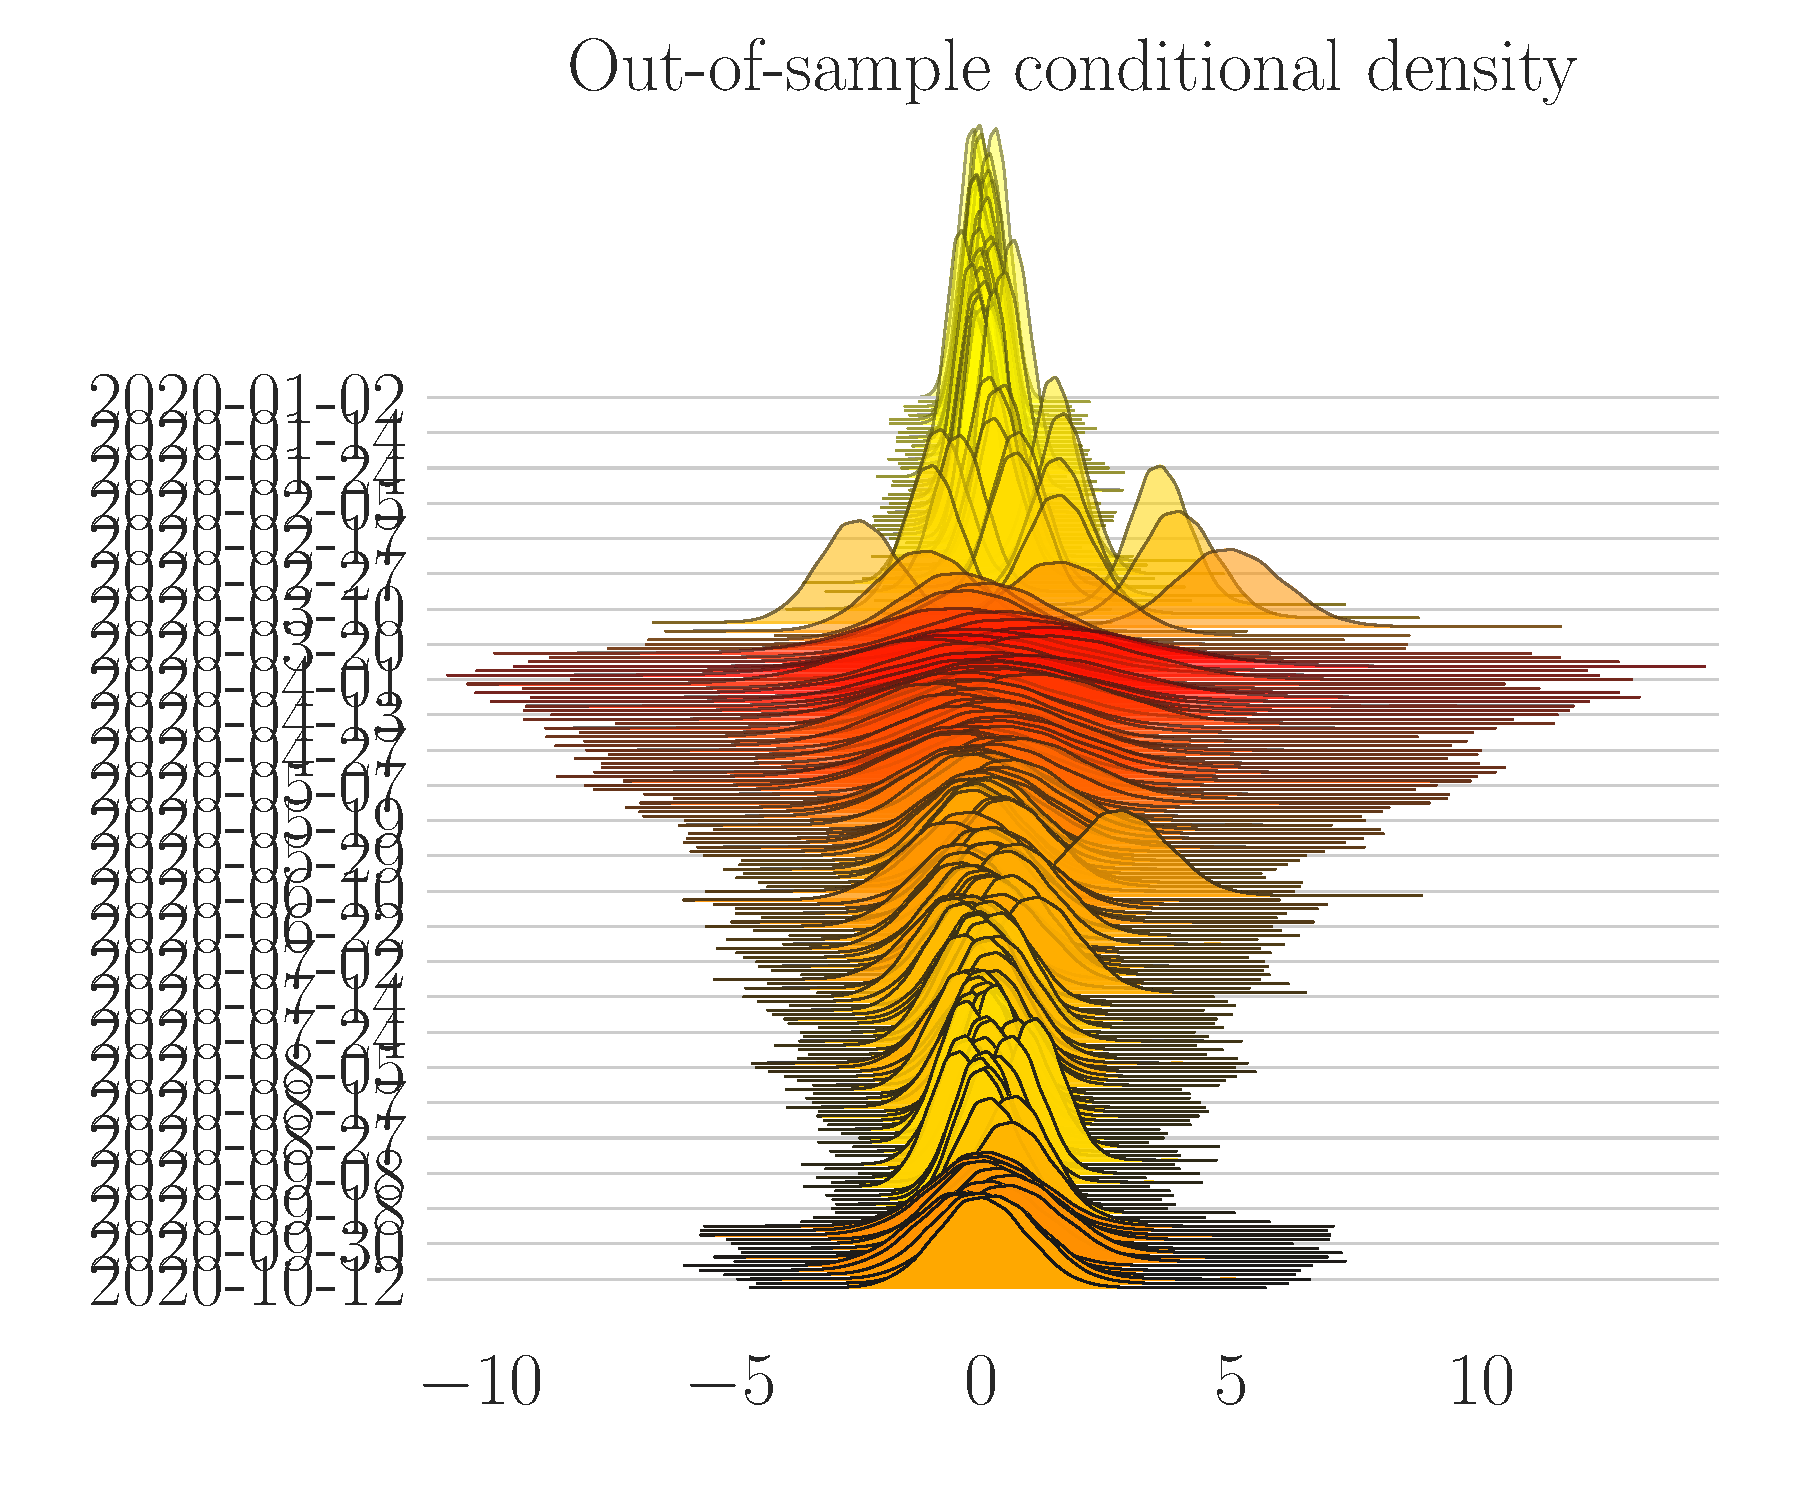
\includegraphics[width=
0.95\textwidth, keepaspectratio]{../output/joyplot.pdf}
\label{fig:joyplot} \source{\emph{Sources}: authors' calculations}
\end{figure}


Like other  types of forecasting density  models, the GARCH model  can also be
used   to   produce  the   so-called   fan   charts,   as  shown   in   Figure
\ref{fig:fanchart}. The  fan chart  presents the  forecasted quantiles  of the
conditional  distribution  across  time  and  provides  an  intuitive  way  to
understand the uncertainty surrounding the  mean forecasts.  In this case, the
uncertainty  is  precisely captured  by  the  GARCH  model, both  through  the
estimation  of the  conditional density  and also  via higher  moments of  the
distribution, including the skewness.\\

\begin{figure} \centering
  \caption{Out-of-Sample  Fan  Chart} 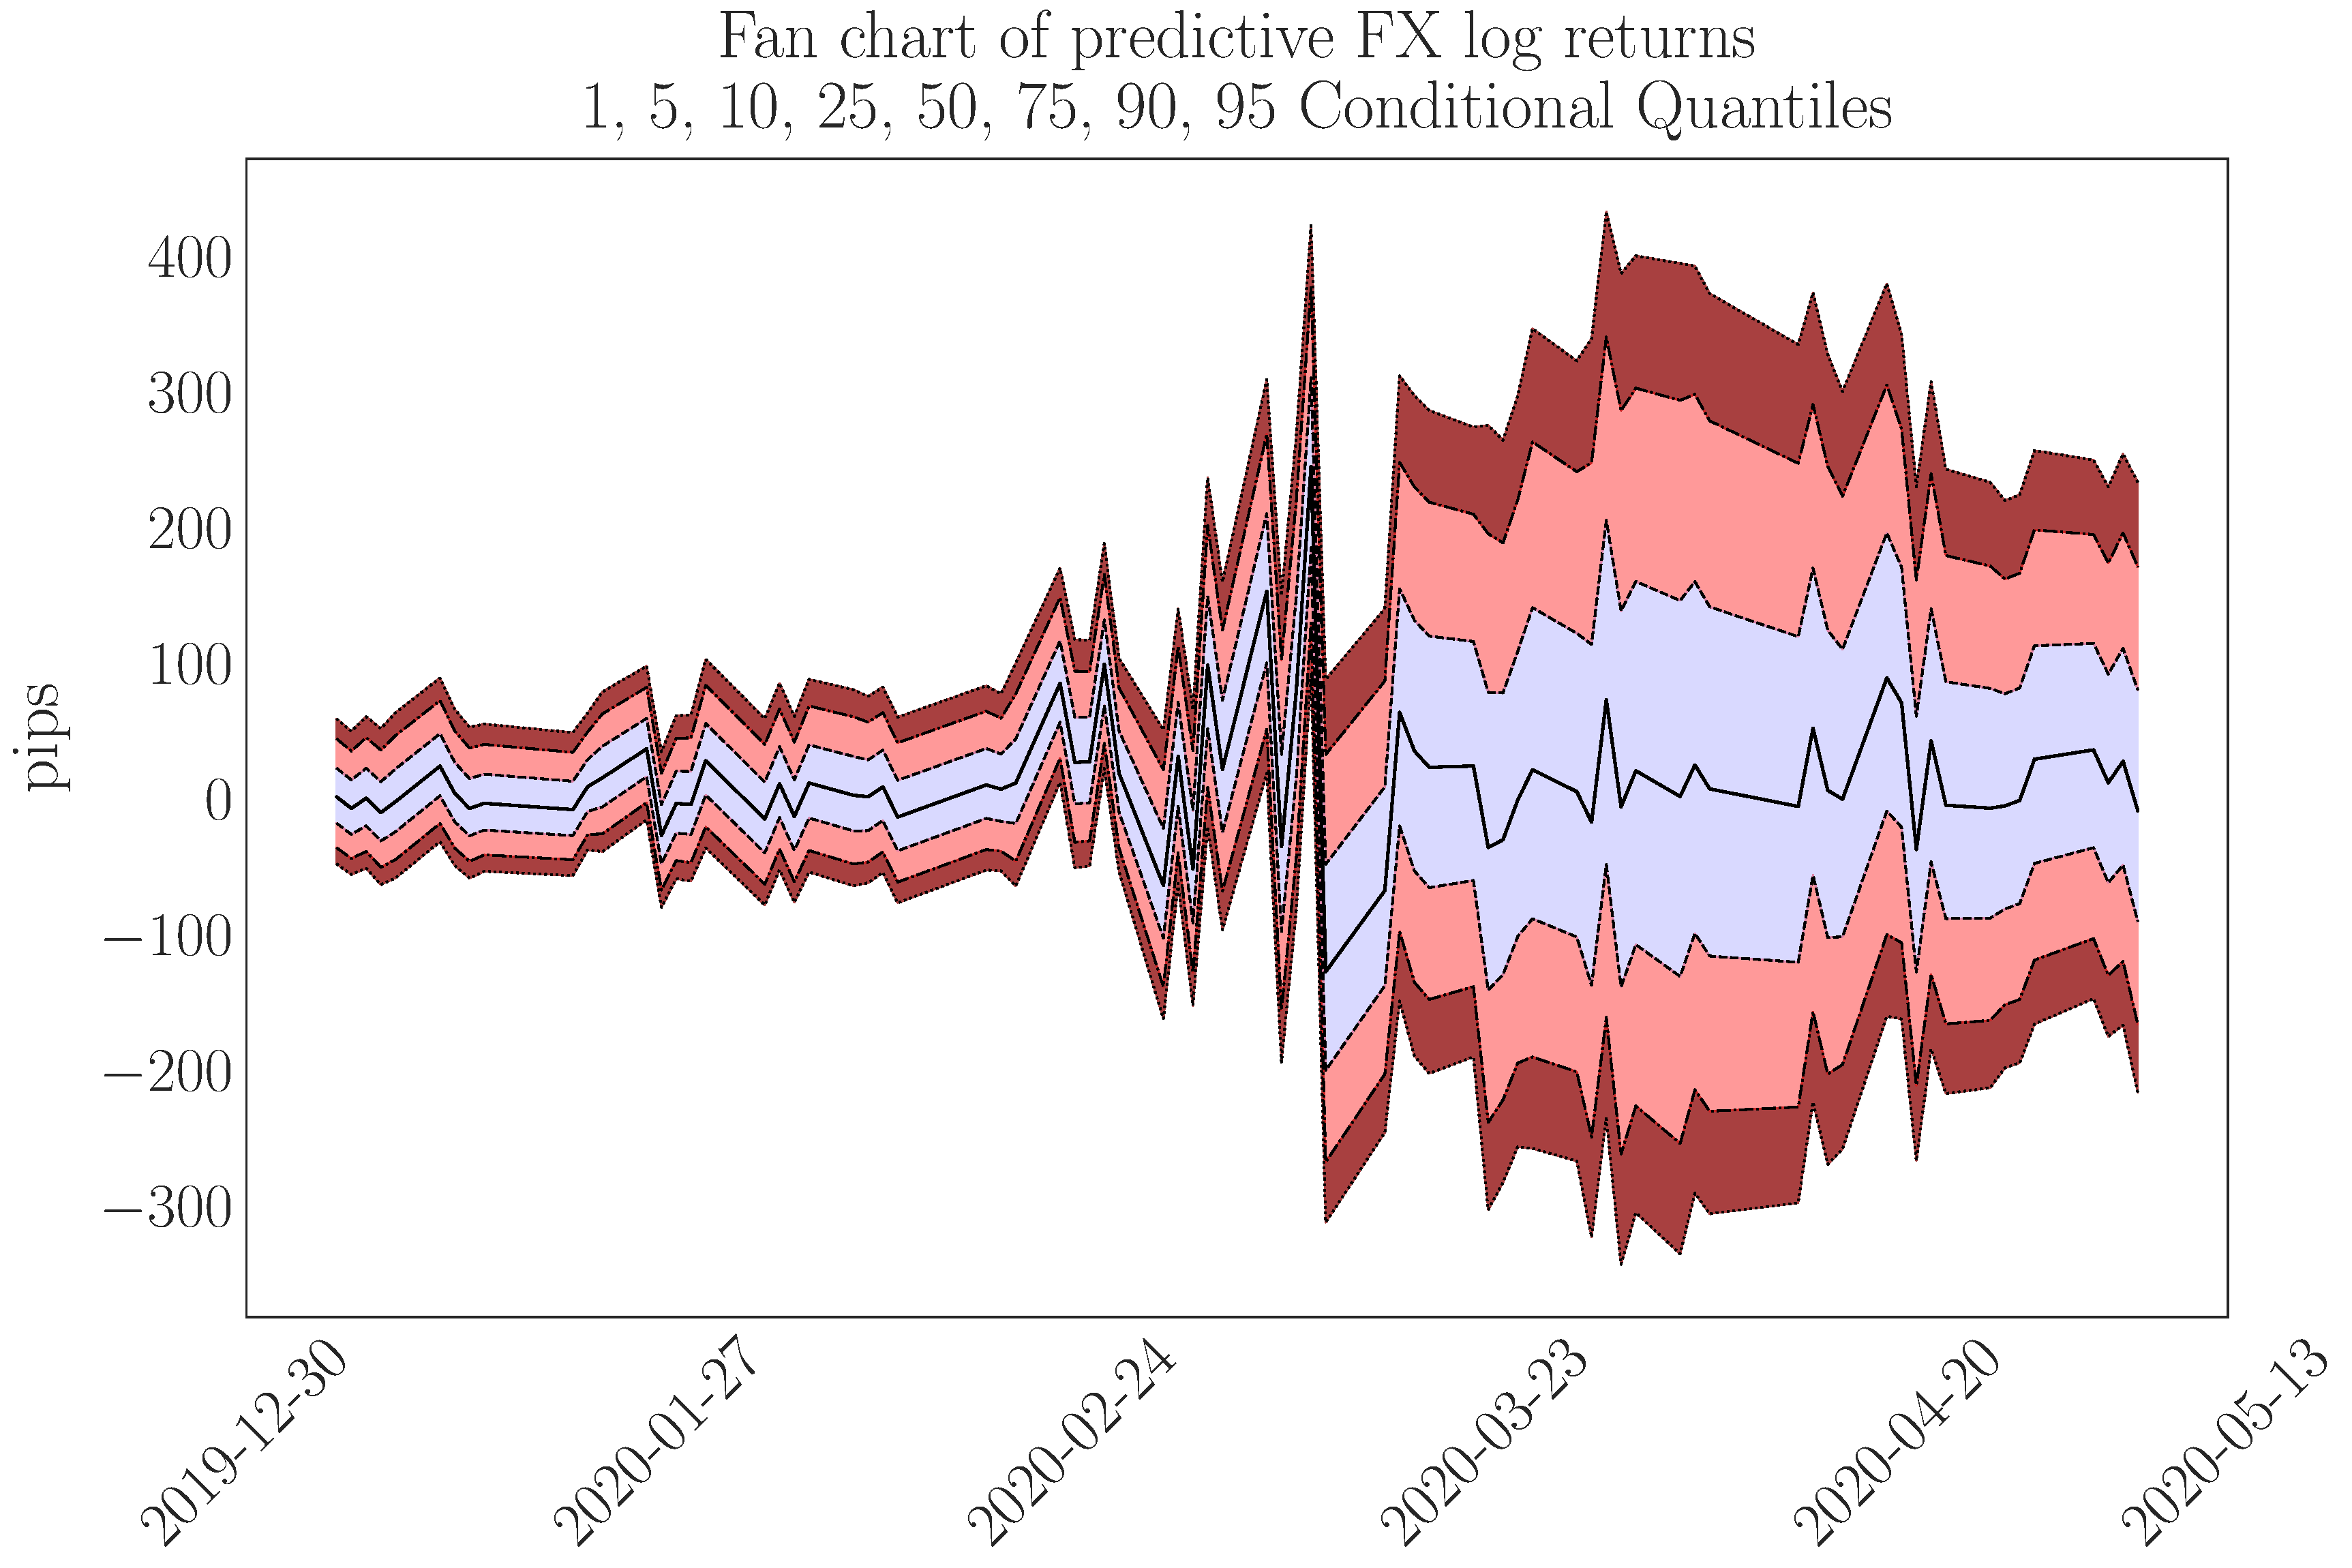
\includegraphics[width=  0.95\textwidth,
keepaspectratio]{../output/fanchart.pdf}
\label{fig:fanchart} \source{\emph{Sources}: authors' calculations}
\end{figure}

Finally,  the quality  of the  GARCH  forecasting density  model is  evaluated
out-of-sample. The correctness of the  density model specification is assessed
via  a   probability  integral   transform  (PIT)   test  (\cite{diebold1998};
\cite{rossi2019}).  The  PIT test  is evaluated over  four-month out-of-sample
daily data,  as presented in  Figure \ref{fig:pitchart}. The PIT  test outcome
presented   in  Figure   \ref{fig:pitchart}  indicates   that  the   empirical
distribution of the PIT is within the confidence band for all quantiles.  This
pattern suggests that the conditional density derived from the EGARCH-X models
has  a  satisfactory  out-of-sample  accuracy and  that  it  generates  robust
predictive distributions that capture well upside and downside risks.\\

Appendix  \ref{sec:benchmarking}  presents  a  series  of  alternative  models
(unconditional via Gaussian kernel,  autoregressive, quantile regressions, and
a series of GARCH and EGARCH  models with different error terms specification)
to benchmark  the performance of our  model, also using log  score performance
metrics  against other  models.  The  result of  the tests  is that  the GARCH
family of  models dominates  the alternative  tested against  an unconditional
kernel density estimator  and conditional density estimated  from the quantile
regression.   Also, within  the GARCH  family (Gaussian,  Tskew, GARCH  versus
EGARCH  for different  error terms  specifications), there  is no  significant
improvement in performance against our baseline model.\\

\begin{figure}
  \centering
  \caption{Probability Integral Transform Test}
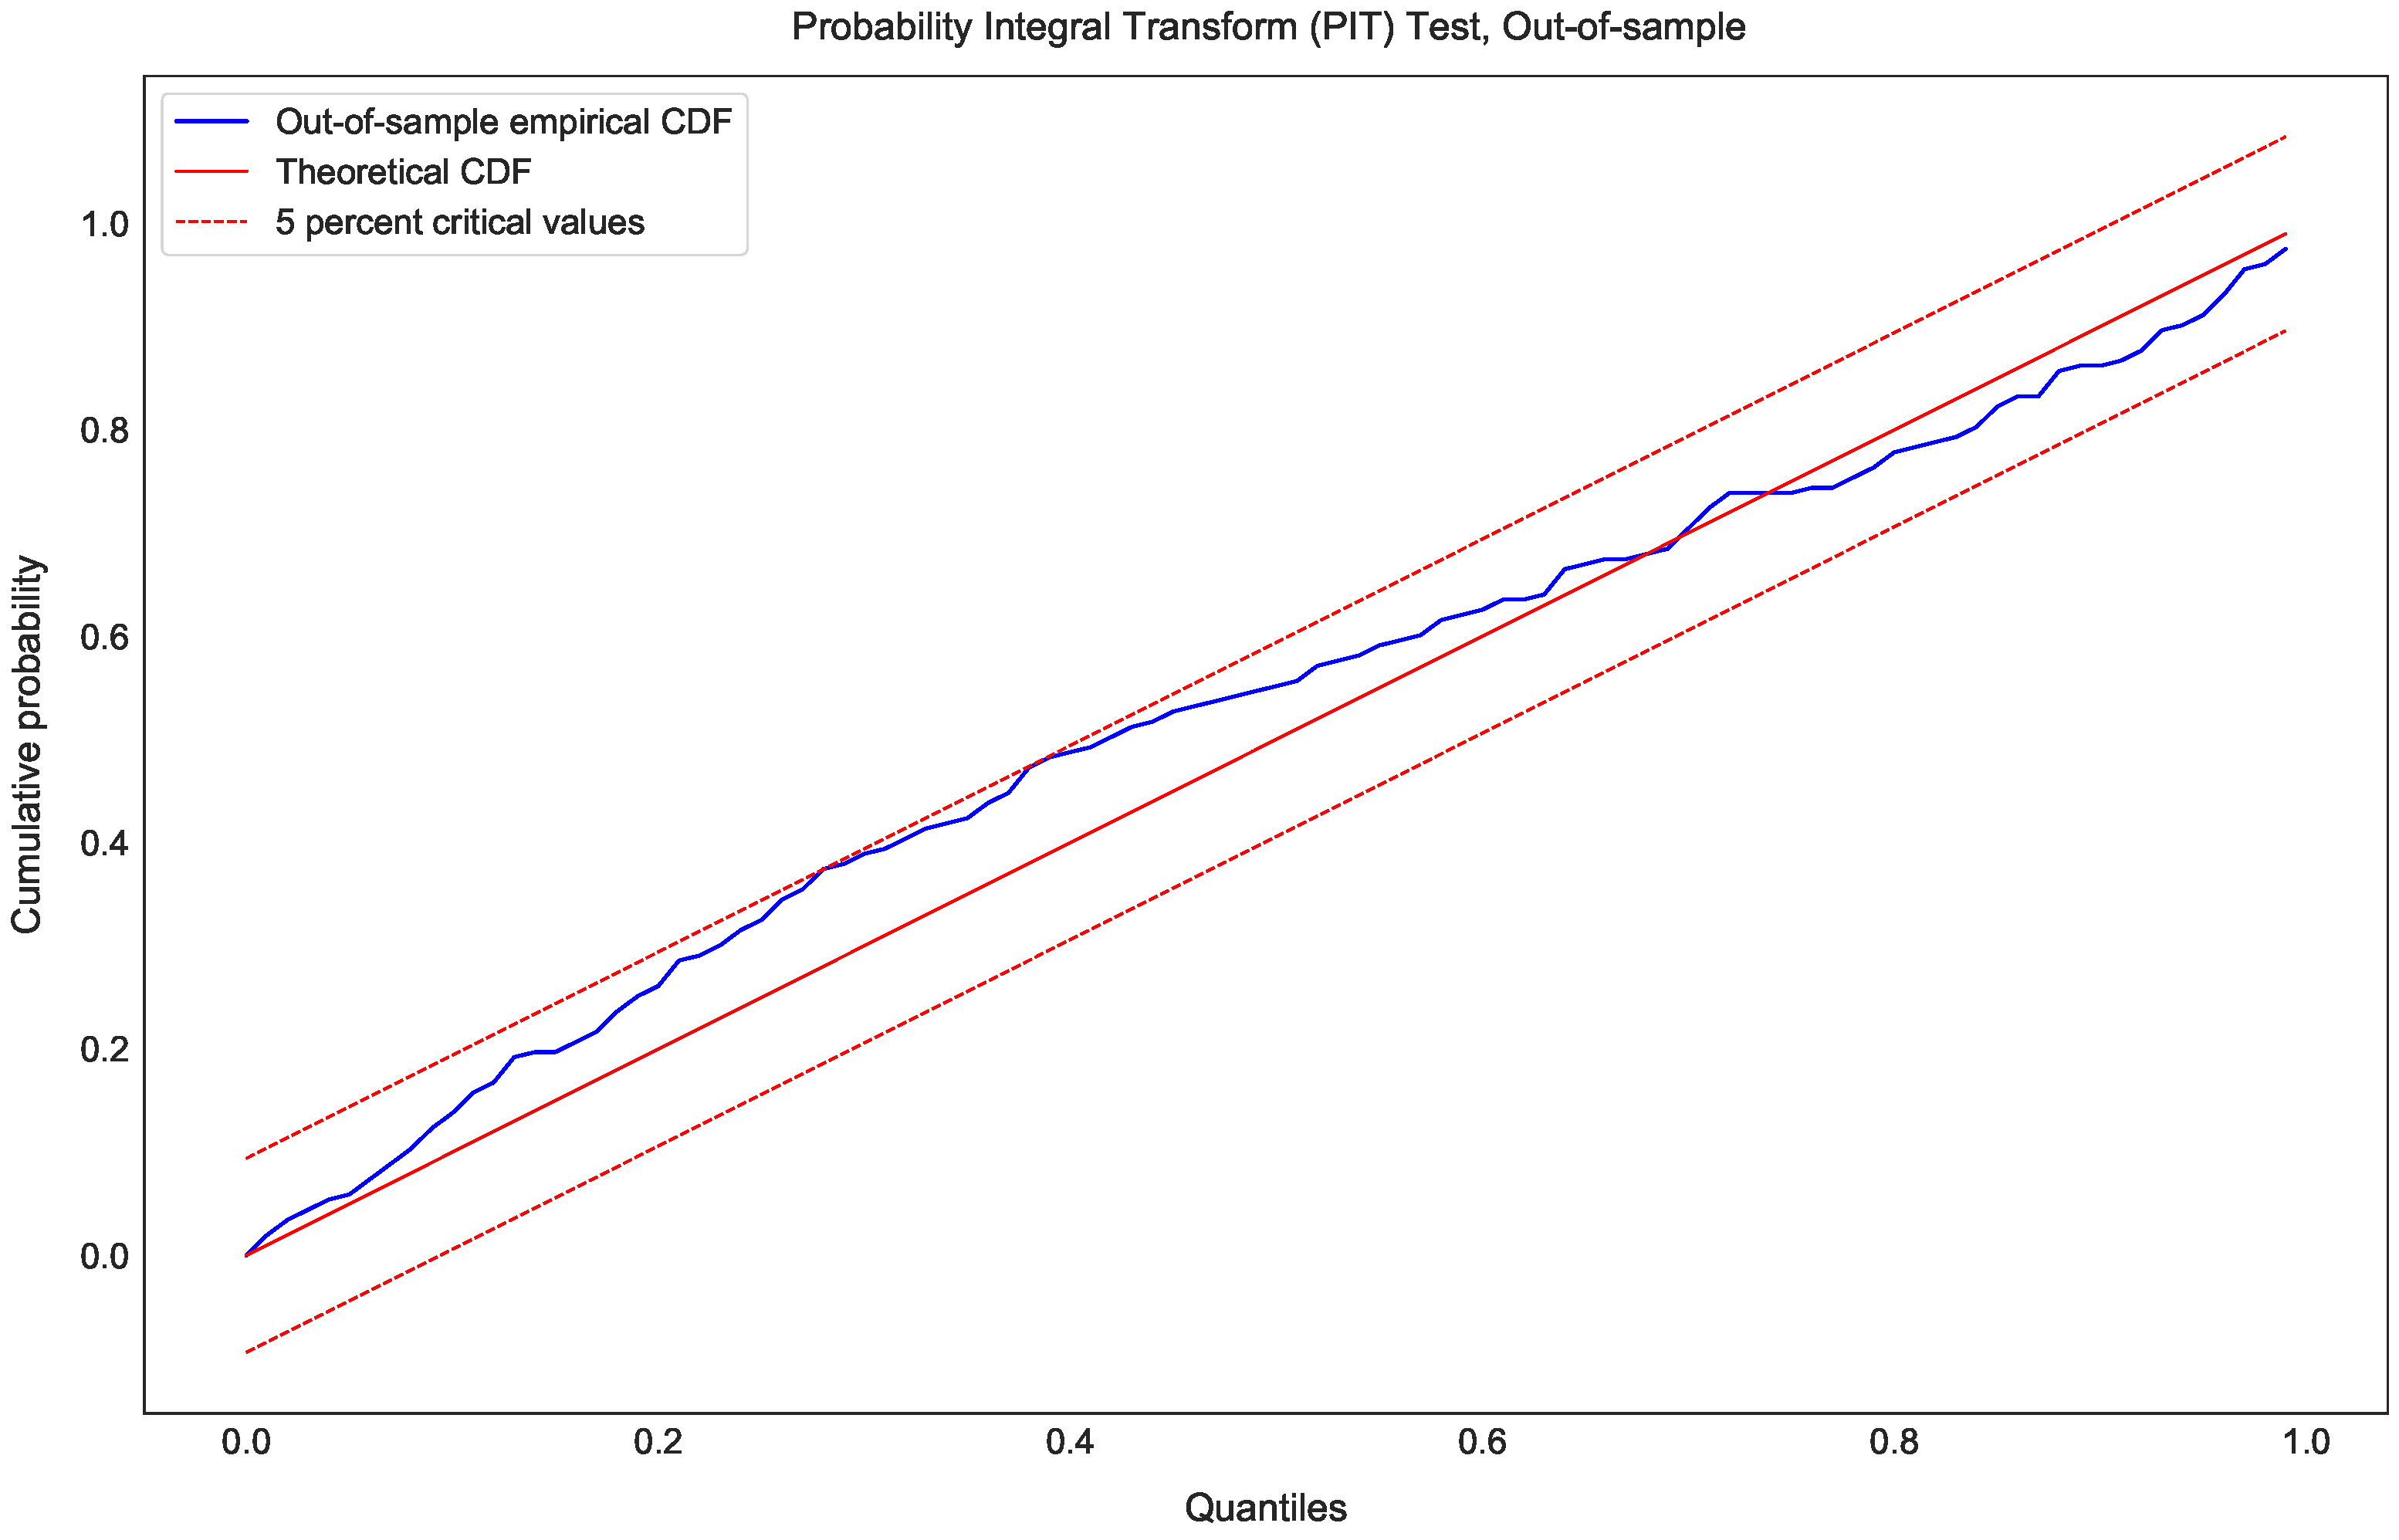
\includegraphics[width= 0.95\textwidth, keepaspectratio]{../output/pitchart.pdf}
\label{fig:pitchart}
\source{\emph{Sources}: authors' calculations}
\end{figure}


%% ---------------------------------------------------------------------------
%% Operational Framework
%% ---------------------------------------------------------------------------
\section{Operational Framework}
\label{sec:operational-framework}


\subsection{Risk-Based Triggers}
\label{sec:triggers}

The VaR rule derives  from a simple time series model  and is, therefore, easy
to operationalize and  to communicate. The model requires a  limited amount of
data,  available   in  the   public  domain,   and  their   interpretation  is
unambiguous. VaR  triggers are transparent  and relatively easy  to understand
and  to  communicate  to  the  market,  while being  part  of  a  more  global
communication strategy  from the central  bank (see, for example,  the Central
Bank Transparency  Code, \cite{imf2020cbt}) FXIs  are performed on
the wholesale market, where participants are  aware of the concept of VaR. The
general  public  might be  less  familiar  with VaR,  but  this  is of  little
consequence  from an  operational standpoint  as the  general public  does not
directly participate in FXI.\\

In practical  terms, the  central bank  estimates the  model and  assesses the
intervention regions  in real  time. The central  bank monitors  the cumulated
returns of the exchange rate—either depreciation or appreciation—compared with
the previous day exchange rate. If more than one intervention per business day
is allowed,  the trigger  for the  second intervention would  be based  on the
cumulated  return of  the exchange  rate compared  with the  previous same-day
trigger rate. For the rest of the  paper, we will assume that the central bank
does not intervene more than once a  day. Once the cumulated returns reach the
intervention regions, the central bank buys  or sells FX. These regions evolve
every day as a function of market conditions. On the specific day presented in
Figure \ref{fig:var-rule},  foreign exchange intervention would  have happened
only  if  the exchange  rate  had  depreciated by  more  than  3.3 percent  or
appreciated by more than 3.7 percent, for a 5 percent VaR (2.5 percent on each
side).  Thresholds would be computed every day, for each possible quantile, as
shown on the fan chart (Figure \ref{fig:fanchart}).\\


\begin{figure}
  \centering
  \caption{VaR FX Intervention Rule Based on a Given Information Set}
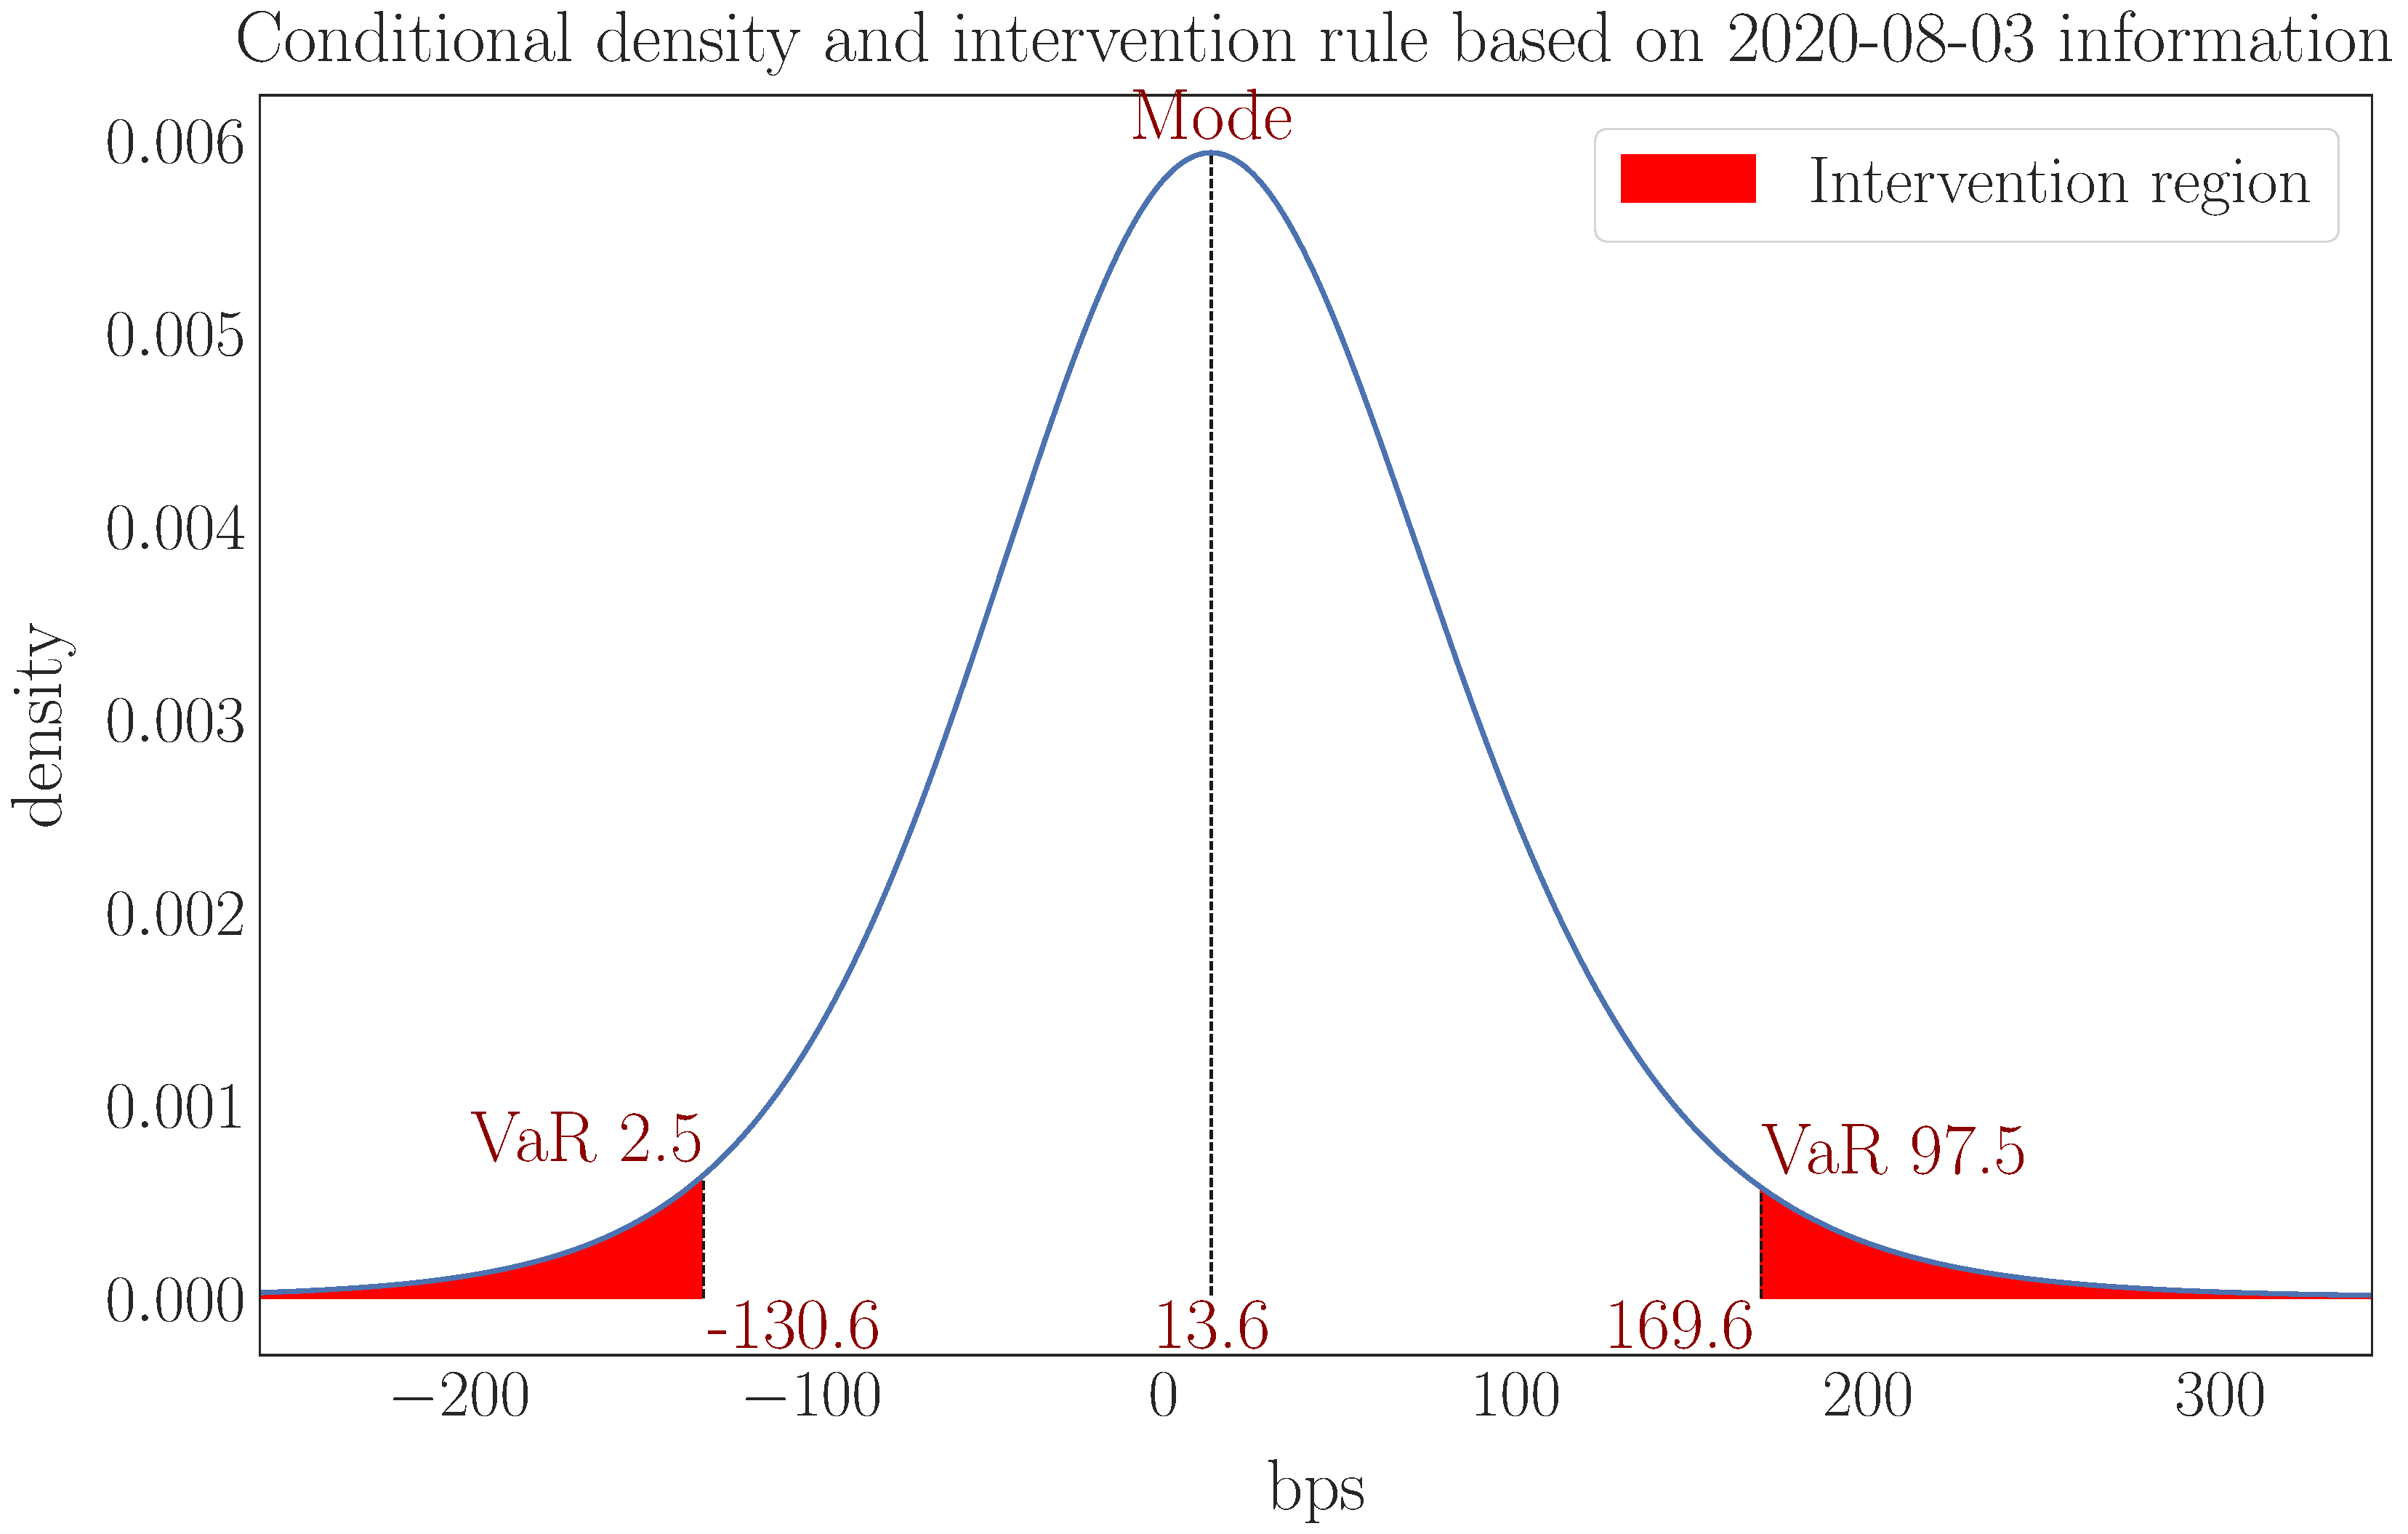
\includegraphics[width= 0.95\textwidth, keepaspectratio]{../output/var_rule.pdf}
\label{fig:var-rule}
\source{\emph{Sources}: authors' calculations}
\end{figure}

Over  time, the  VaR-FXI  rule can  be  represented by  the  region where  the
cumulative  distribution   function  falls  outside  the   central  bank  risk
tolerance,  for example,  the 2.5th  and 97.5th  percentiles, as  presented in
Figure \ref{fig:conditional-cdf}.\\

\begin{figure}
  \centering
  \caption{Conditional Cumulative Distribution Function and Intervention Thresholds}
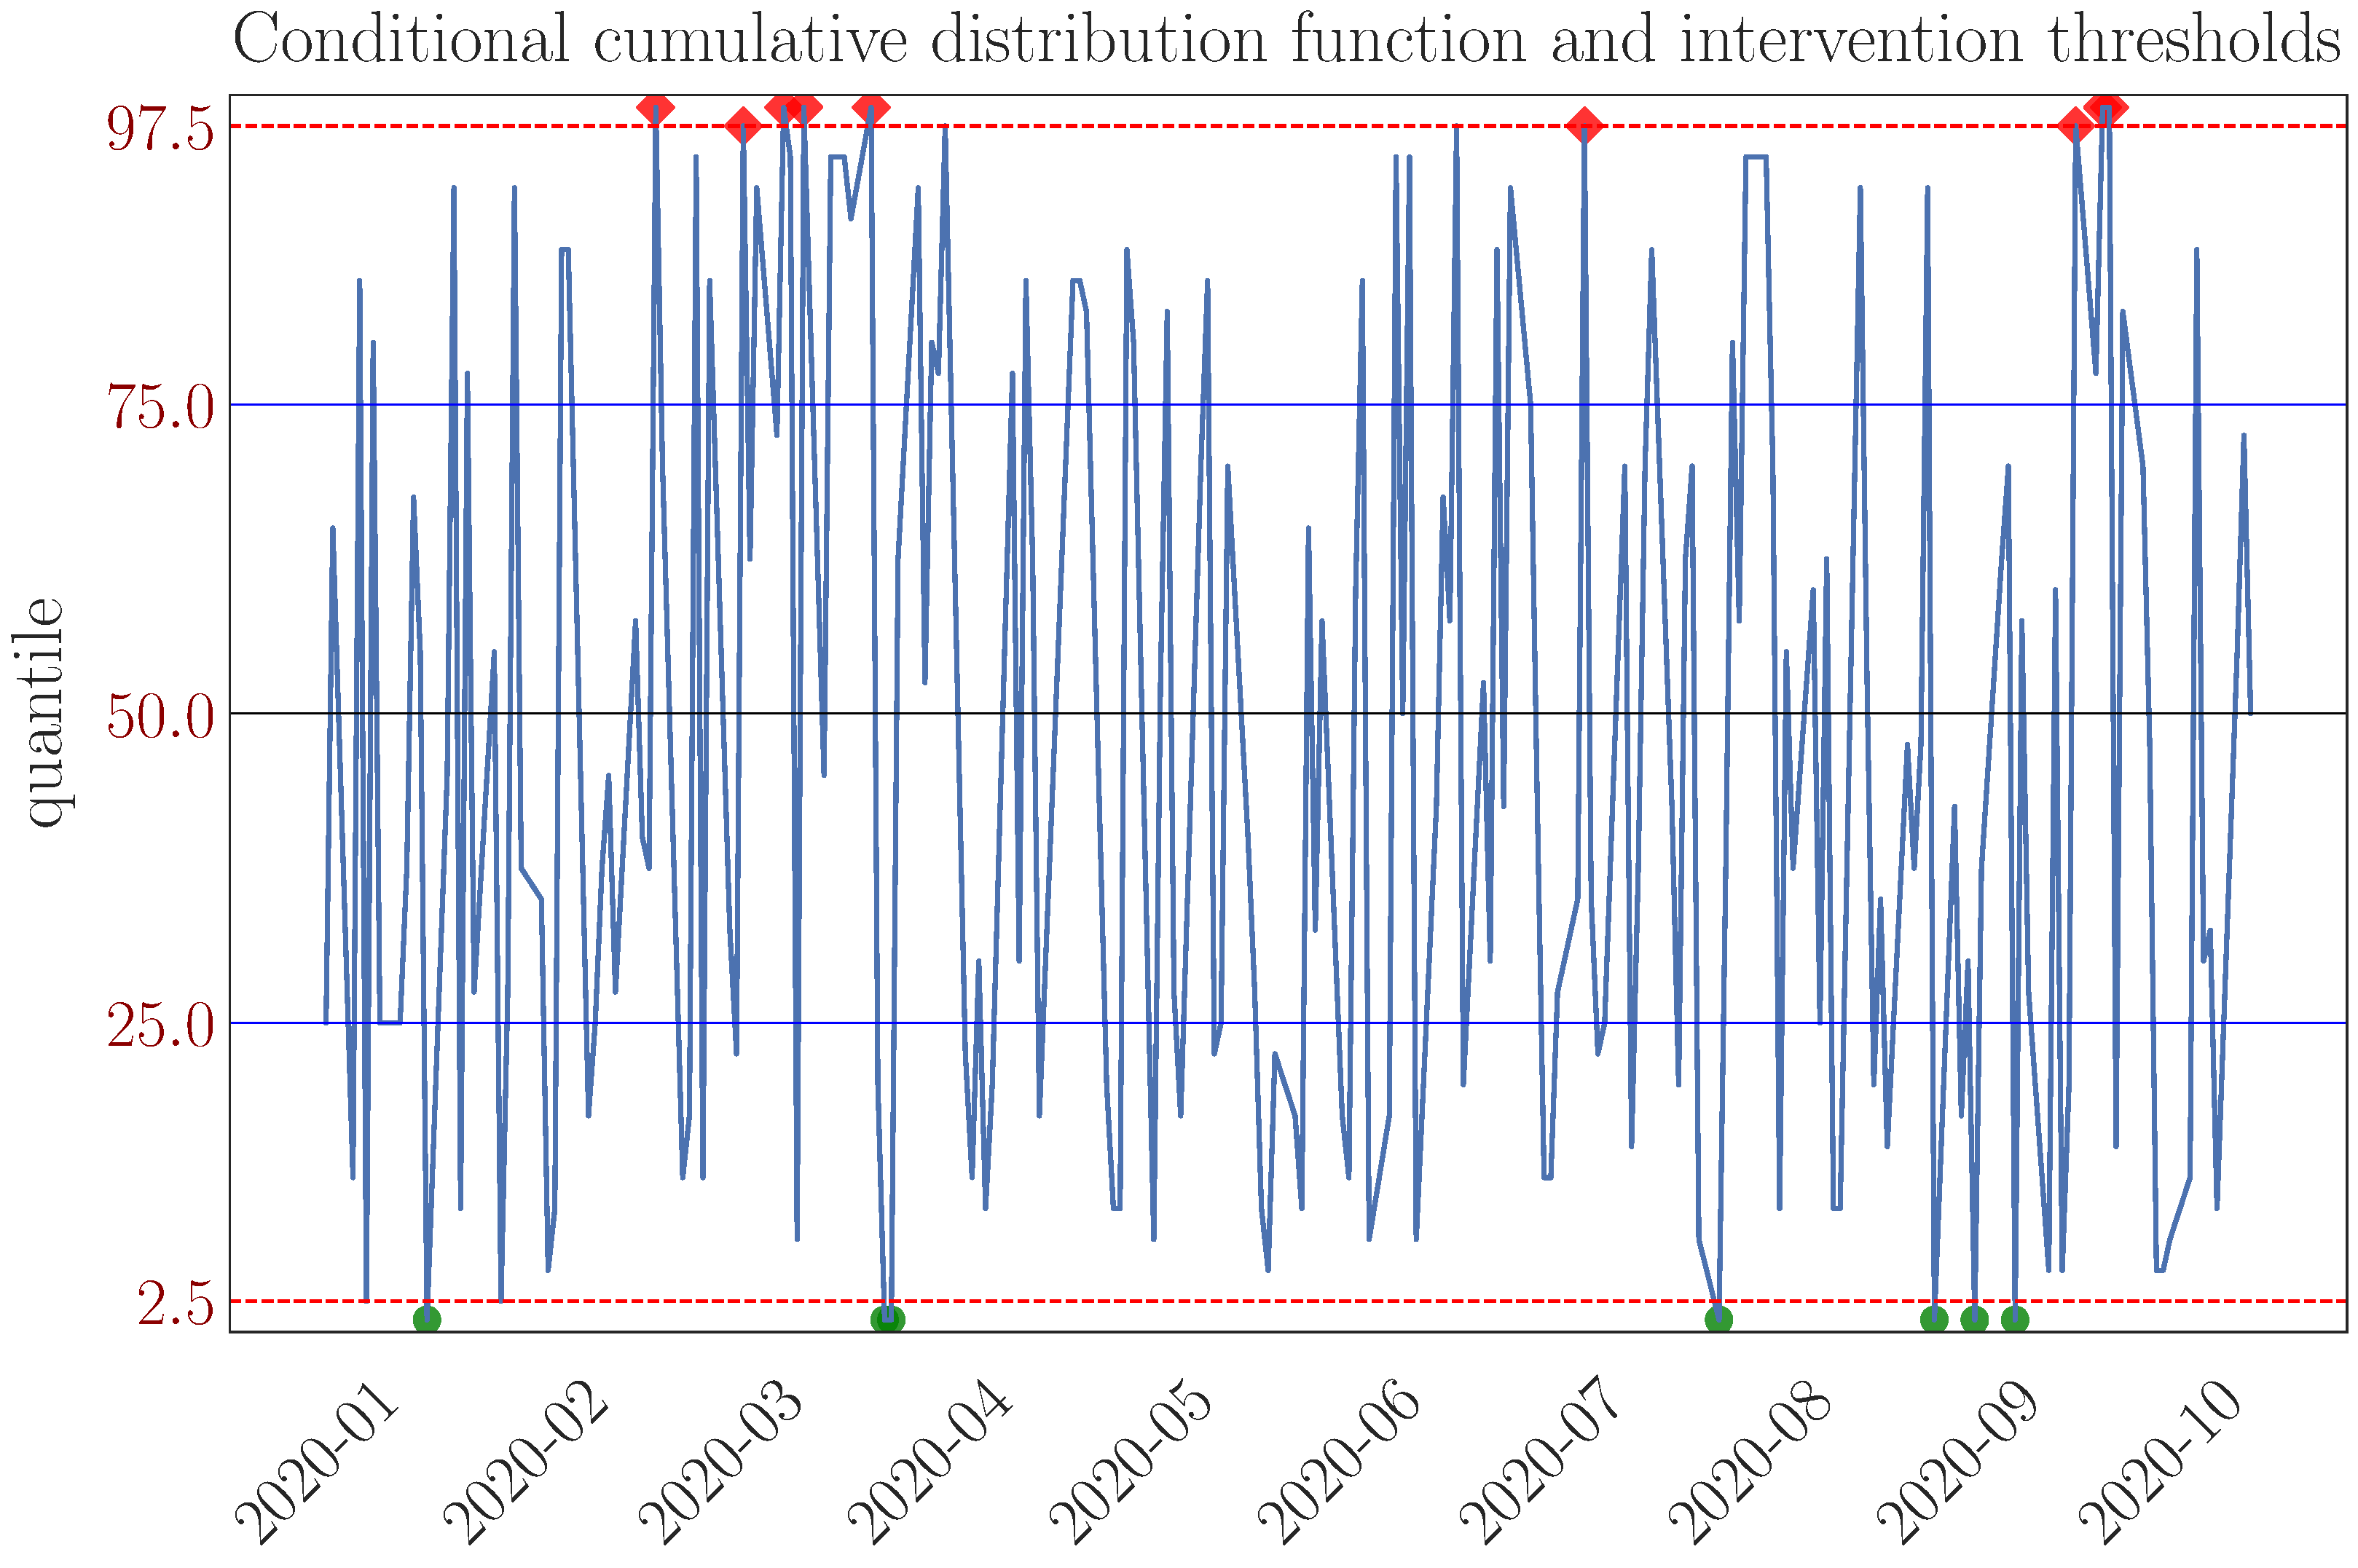
\includegraphics[width= 0.95\textwidth, keepaspectratio]{../output/conditional_cdf.pdf}
\label{fig:conditional-cdf}
\source{\emph{Sources}: authors' calculations}
\end{figure}

Had the BM followed the VaR FX  intervention rule, it might have intervened in
about  15 days  over 10  months, from  January through  October 2020.   Figure
\ref{fig:conditional-exceedance}  presents the  intervention  days within  the
daily  log-returns plot.   It highlights  with  green dots  (below ERaR  2.5th
percentile) and  red dots (above  the ERaR 97.5th percentile)  the occurrences
falling   in   the  intervention   regions.   The   lower  chart   of   Figure
\ref{fig:conditional-exceedance} presents the corresponding  FX level in which
the  central  bank  would  have   intervened.  Fifteen  days  of  intervention
correspond to about 7.5 percent of the period, even when using an intervention
region  of 5  percent.  The  frequency  of interventions  would increase  when
volatility  is  unusually  high,  which  was  the  case  during  the  COVID-19
crisis. However, this exercise is purely counterfactual, and it is likely that
after the first FX intervention, the FX volatility would have decreased, hence
reducing the need for future interventions.\\

\begin{figure}
  \centering
  \caption{Conditional VaR Exceedance, Out-of-Sample}
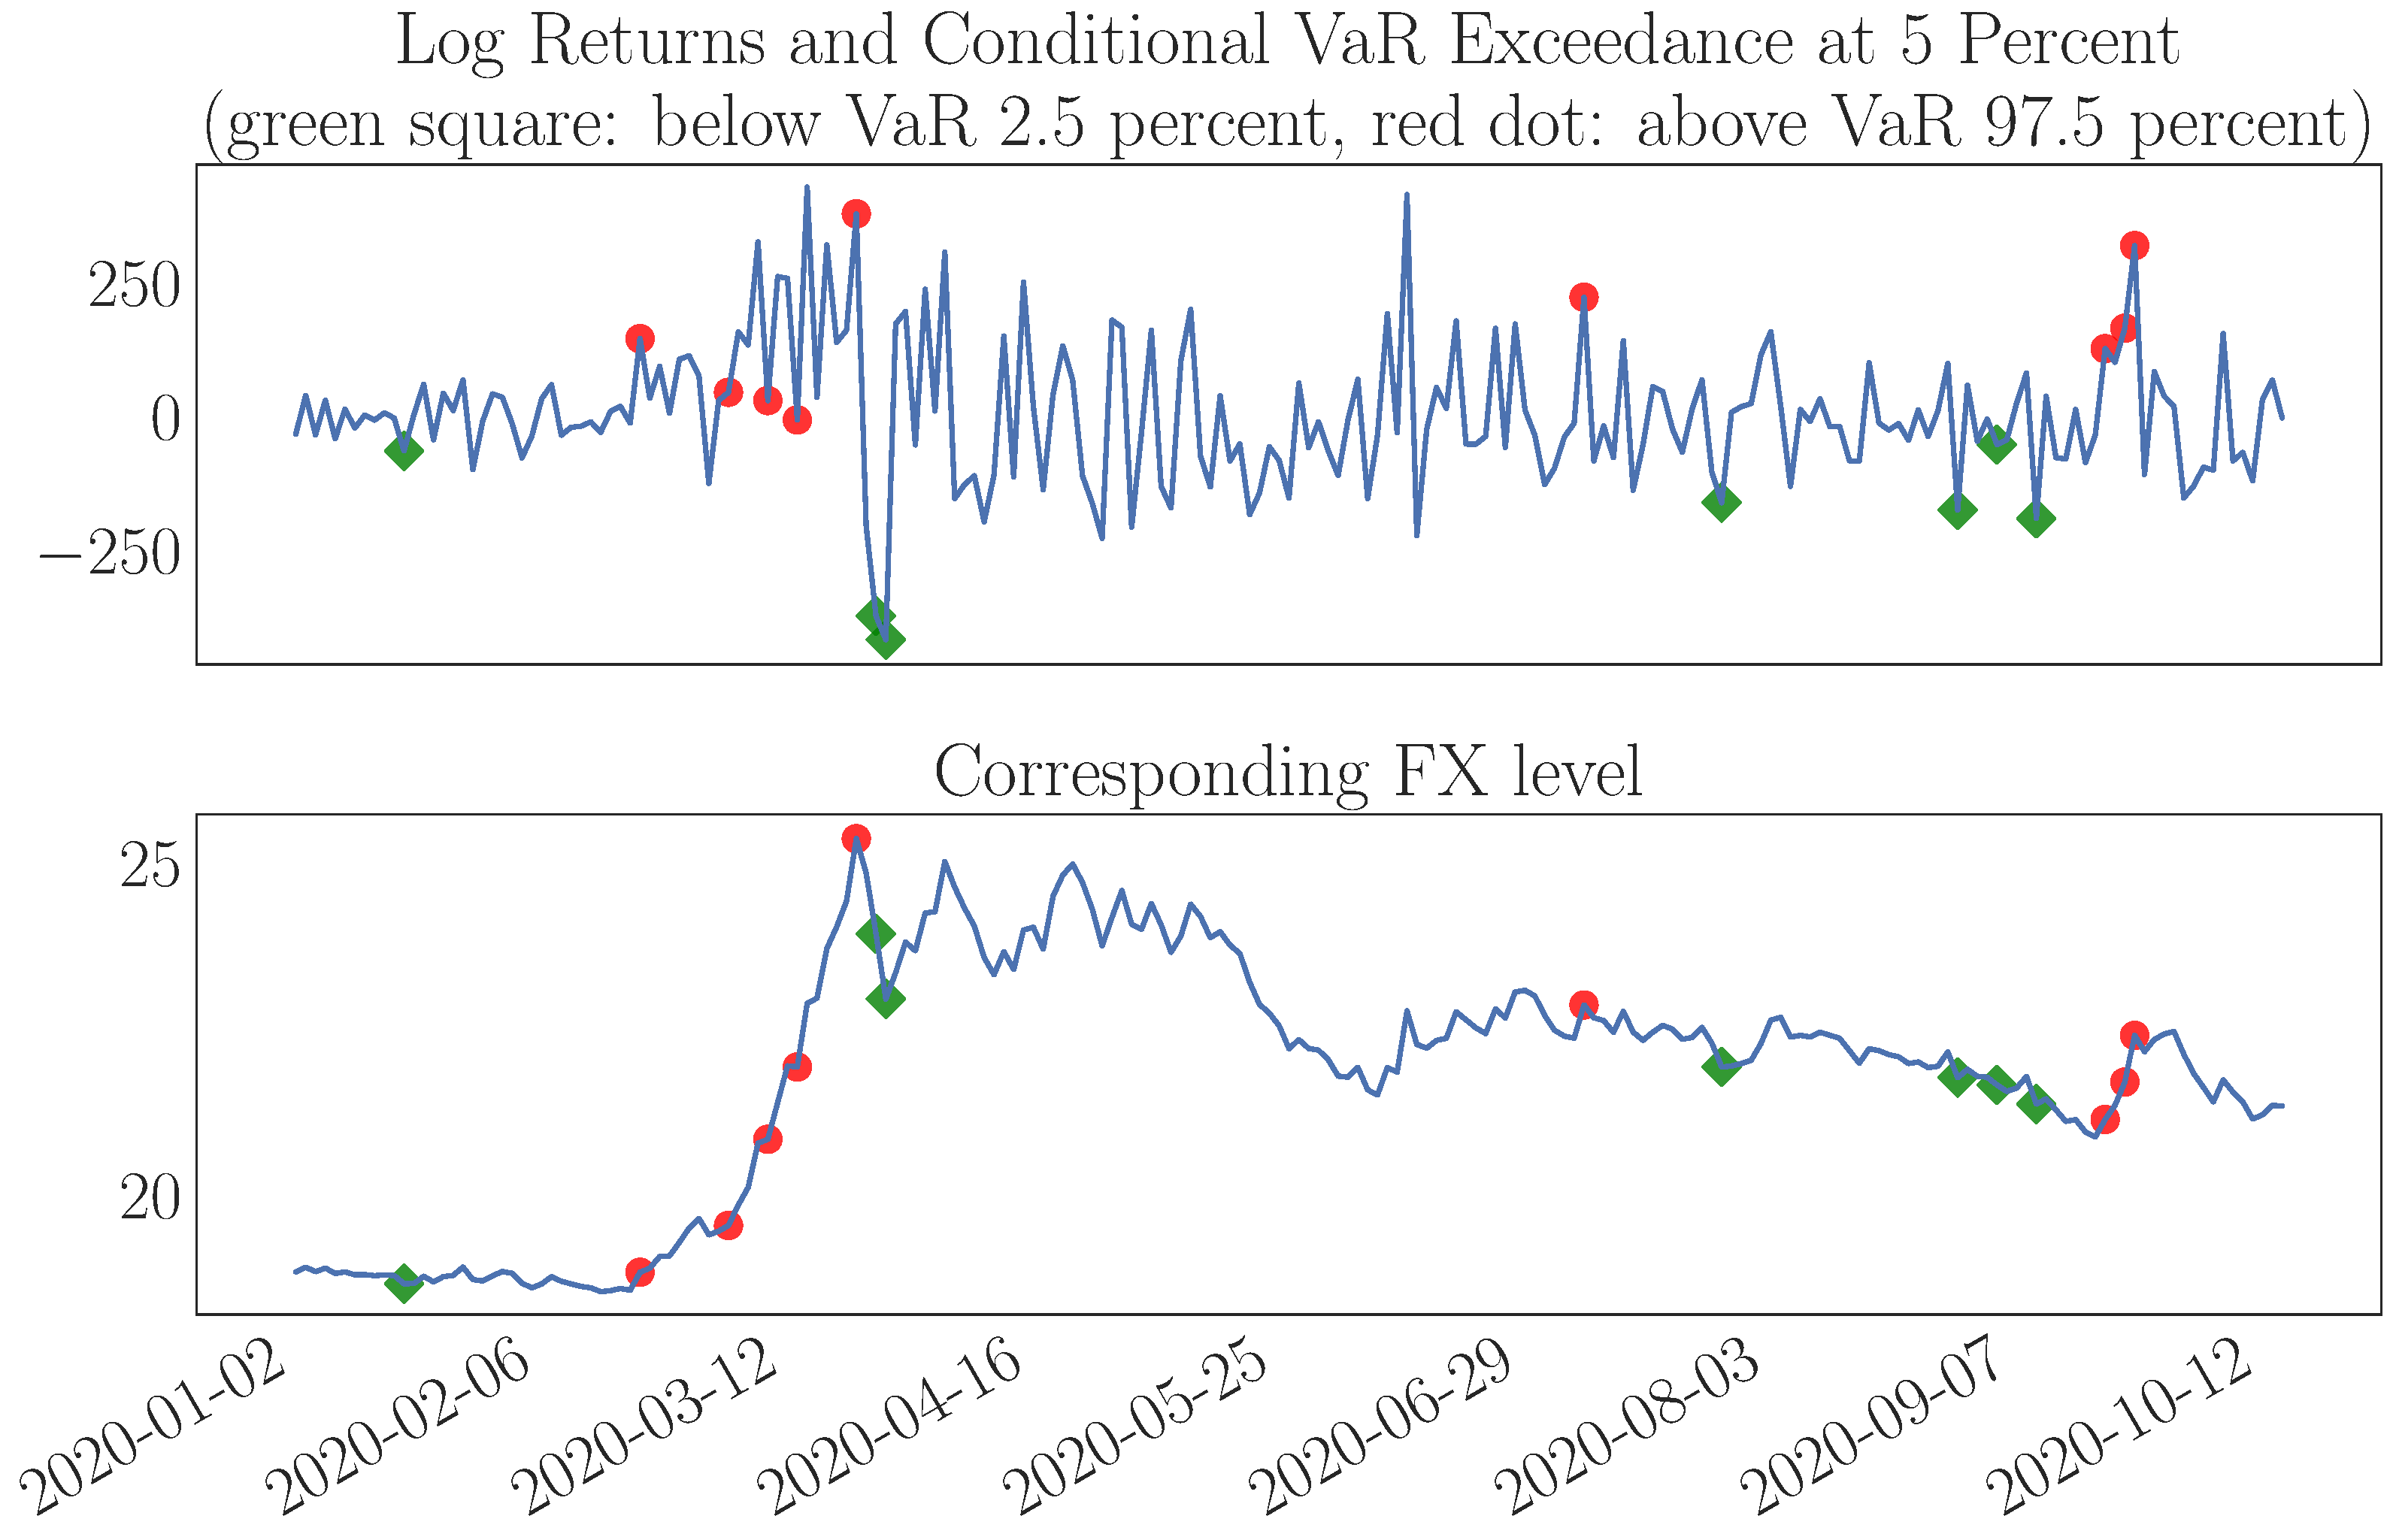
\includegraphics[width= 0.95\textwidth, keepaspectratio]{../output/conditional_exceedance.pdf}
\label{fig:conditional-exceedance}
\source{\emph{Sources}: authors' calculations}
\end{figure}

\subsection{FX Intervention Calibration under Risk-Based Interventions}
\label{sec:calibration}

One of  the major  advantages of the  VaR rule is  that it  provides certainty
about the frequency of FXIs over time.  For example, with a VaR of 2.5 percent
both for depreciation and appreciation, the  central bank will, on average and
over time,  intervene 5  percent of  the time.  The central  bank intervention
frequency might temporarily  deviate over a short period  of time―depending on
market conditions―but  the VaR approach  guarantees that the frequency  is the
same as the VaR over a sufficiently long period of time.\\

The  fixed-frequency feature  of the  VaR rule  can be  used to  calibrate the
central banks’  intervention budget.  We assume  that the  central bank  set a
maximum amount for its intervention, which  can be set for single intervention
or  for  one   business  day  (the  later  is  often   consider  as  the  most
practical).  The  budget could,  then,  be  directly  derived from  the  fixed
frequency of intervention and the maximum FXI amount. The budget should remain
within the constraint represented by the  available FX reserves at the central
bank for FXI. This is an important advantage compared to fixed-volatility rule
where interventions  frequency and,  thus, the  interventions budget,  are not
known ex-ante.\\

The  VaR rule  could  contribute to  the  improve the  efficiency  of FXIs  by
maximizing  the  impact  on  the  exchange  rate for  a  given  amount  of  FX
sold/bought  by the  central bank.  The maximum  amount of  daily intervention
should be  large enough to influence  the exchange rate when  the central bank
intervenes. Accepting higher VaR (lower  intervention frequency) is a solution
if the intervention budget exceeds the FX reserves availability constraint, to
keep the daily  intervention at a credible amount. Another  feature of the VaR
rule  is that  it triggers  interventions  when price  movement are  unusually
large, which should reinforce the intervention impact on the exchange rate.\\

Another  substantial  benefit  of  the  VaR  rule  is  that  it  improves  the
sustainability of the  intervention policy. Should the central  bank decide to
operate  with   a  symmetric   rule  (the  same   VaR  for   appreciation  and
depreciation), it will intervene the same number of times on both sides, hence
offsetting selling FX with  buying FX over time. As a  result, a symmetric VaR
rule would be budget neutral for the central bank over the medium term.\\


%% ---------------------------------------------------------------------------
%% The Case of Mexico
%% ---------------------------------------------------------------------------

\section{The Case of Mexico}
\label{sec:mexico-case}

The BM  intervened via two types  of auctions which differ  by the reservation
rate applied to each  type of auctions. In the first type,  the BM operated an
auction every day  with a preannounced reservation rate, that  is, the minimum
rate               for               eligible               bids.\footnote{See
\url{https://www.banxico.org.mx/markets/auctions-with-minimum-price-e.html}
for  more details}  On many  days, the  auction with  a minimum  rate did  not
receive any demand, as the market was operating below the reservation rate. In
the second type, the auction was organized  when the BM found it opportune and
did not have a reservation rate (an auction without a minimum rate).  For some
periods (for example, during 2015), daily auctions were preannounced without a
minimum  rate.   The   auctioned  amount  was  also   preannounced  and  later
adjusted.\\

We are  focusing in  this paper on  benchmarking the BM's  FXI against  a risk
framework, while  recognizing that the BM  could have had other  objectives in
mind. The BM may have intervened  for other reasons than preventing disorderly
market conditions.  The  exact rationales for FXI is outside  the scope of the
paper. We  are not  assessing, here,  the efficiency,  the relevance,  nor the
rationale of the BM's interventions.\\


\subsection{Interventions with a Minimum Price}
\label{sec:min-price}

"Auctions with  a minimum  price" were  triggered 31  times from  October 2008
through November 2016.  The auction reservation  price was set at the previous
day's  exchange   rate  close   (MEX/USD)  multiplied   by  1.02   (2  percent
depreciation)  from October  9,  2008,  to December  8,  2014,  by 1.015  from
December 9, 2014, to November 23, 2015, and by 1.01 from November 24, 2015, to
January 5, 2017. Auctions with a minimum price were suspended after January 5,
2017. Figure \ref{fig:benchmark-minprice} presents the auctions with a minimum
price in green, with the corresponding FX daily log returns and level.\\

\begin{figure} \centering
  \caption{FX    Interventions    Log     Returns    with    Minimum    Price}
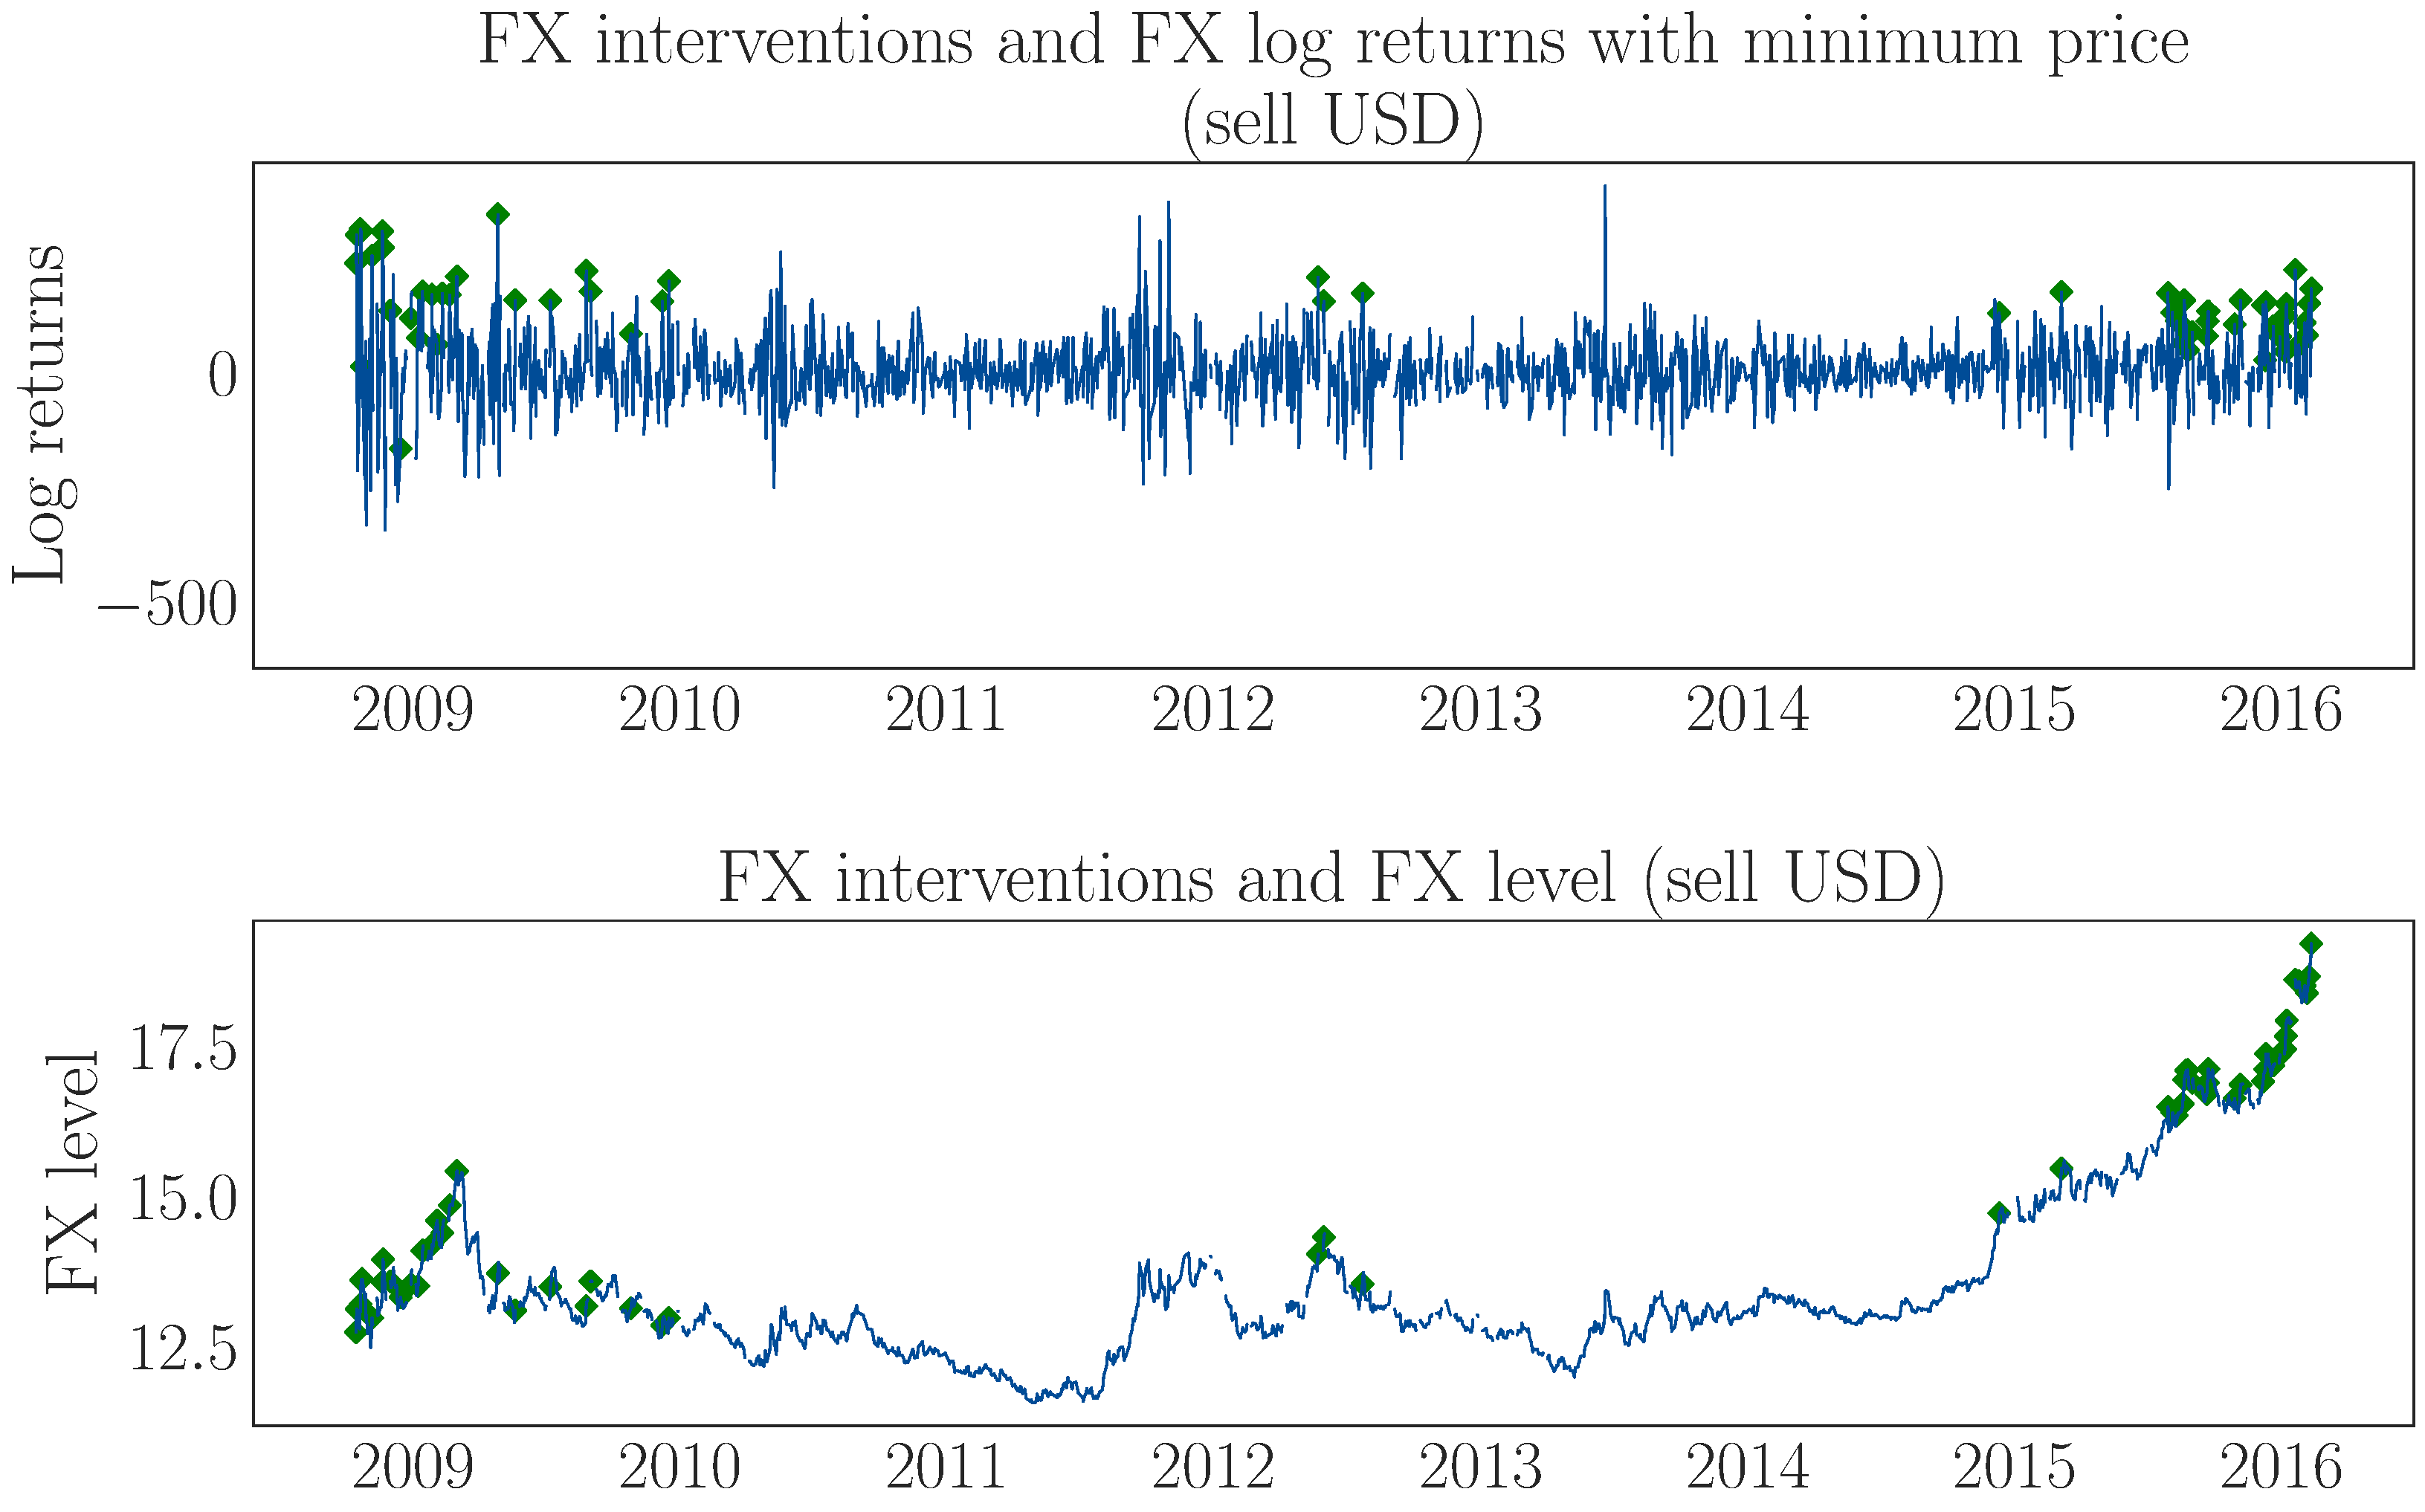
\includegraphics[width=                                        0.95\textwidth,
keepaspectratio]{../output/benchmark_minprice.pdf}
\label{fig:benchmark-minprice}   \source{\emph{Sources}:   Banco  Mexico   and
authors' calculations}
\end{figure}

The ex-ante  conditional cumulative distribution function  (CDF) estimated via
the   GARCH   model    is   used   to   benchmark   the    Banco   Mexico   FX
interventions. Although the  central bank did not use the  model to intervene,
one can always assess the corresponding  FX rate conditional quantile when the
central   bank  has   intervened.   The   outcome  is   presented  in   Figure
\ref{fig:benchmark-minprice-cdf}.  The  back-testing exercise shows  that most
FX   interventions   have   occurred   on   the   top   of   the   conditional
distribution―where the depreciation  was the largest―and often  above the 95th
percentile. A few outliers  occur at the median or below,  but these cases are
rare. Overall,  the interventions with  the minimum price approach  were often
but not  always equivalent to  a risk  framework: the central  bank intervened
most of the time when the pressure  on the exchange rate was the largest, with
exceptions.\\

\begin{figure} \centering
  \caption{Conditional   CDF   of   FX  Intervention   with   Minimum   Price}
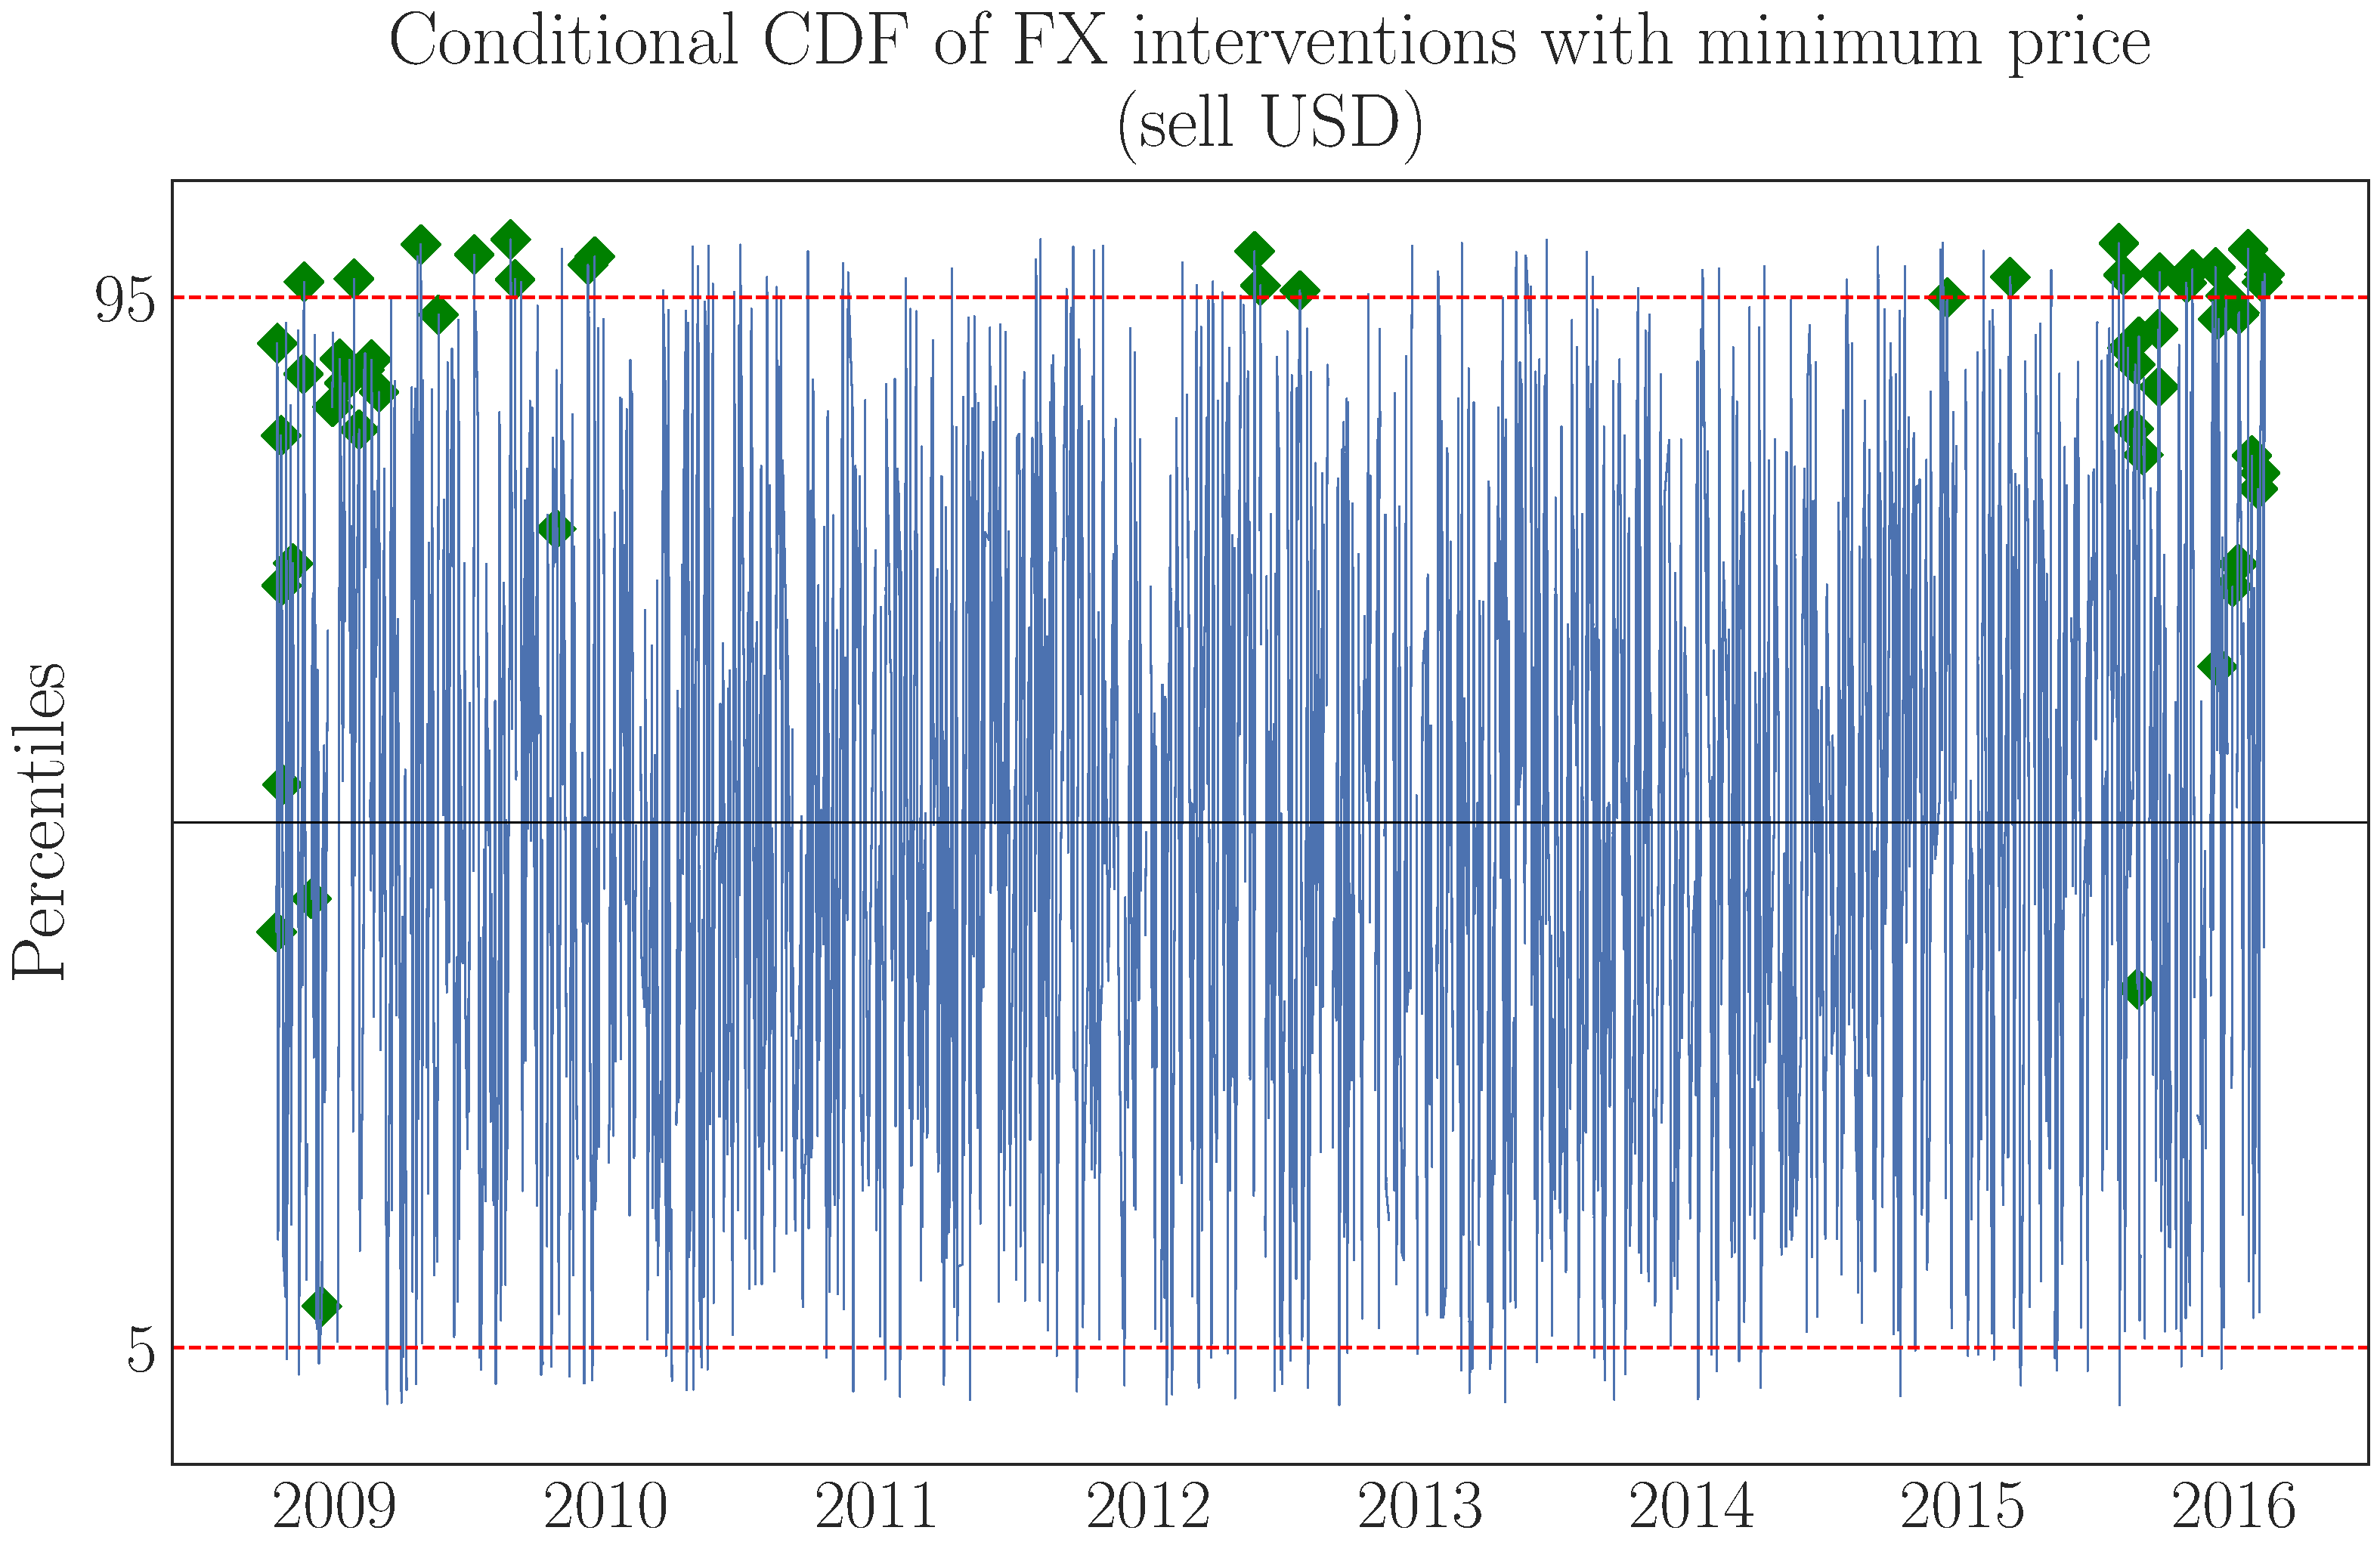
\includegraphics[width=                                        0.95\textwidth,
keepaspectratio]{../output/benchmark_minprice_cdf.pdf}
\label{fig:benchmark-minprice-cdf}  \source{\emph{Sources}:  Banco Mexico  and
authors' calculations}
\end{figure}


\subsection{Interventions without a Minimum Price}
\label{sec:nomin-price}

The BM  organized 319 "auctions without  a minimum price" from  September 2009
through November 2015.  Interventions without  a minimum price overlapped with
"auctions  with  a  minimum  price,"  which  could  constrain  the  volatility
distribution even  in the  absence of actual  intervention under  the rule―the
mere presence  of the  rule influences  market participants'  behavior. Figure
\ref{fig:benchmark-nominprice} presents the FX interventions without a minimum
price on the Mexican pesos in red, with the corresponding FX daily log returns
and level.\\

\begin{figure} \centering
  \caption{FX Interventions  without a  Minimum Price  on the  Mexican Peso/US
Dollar}                 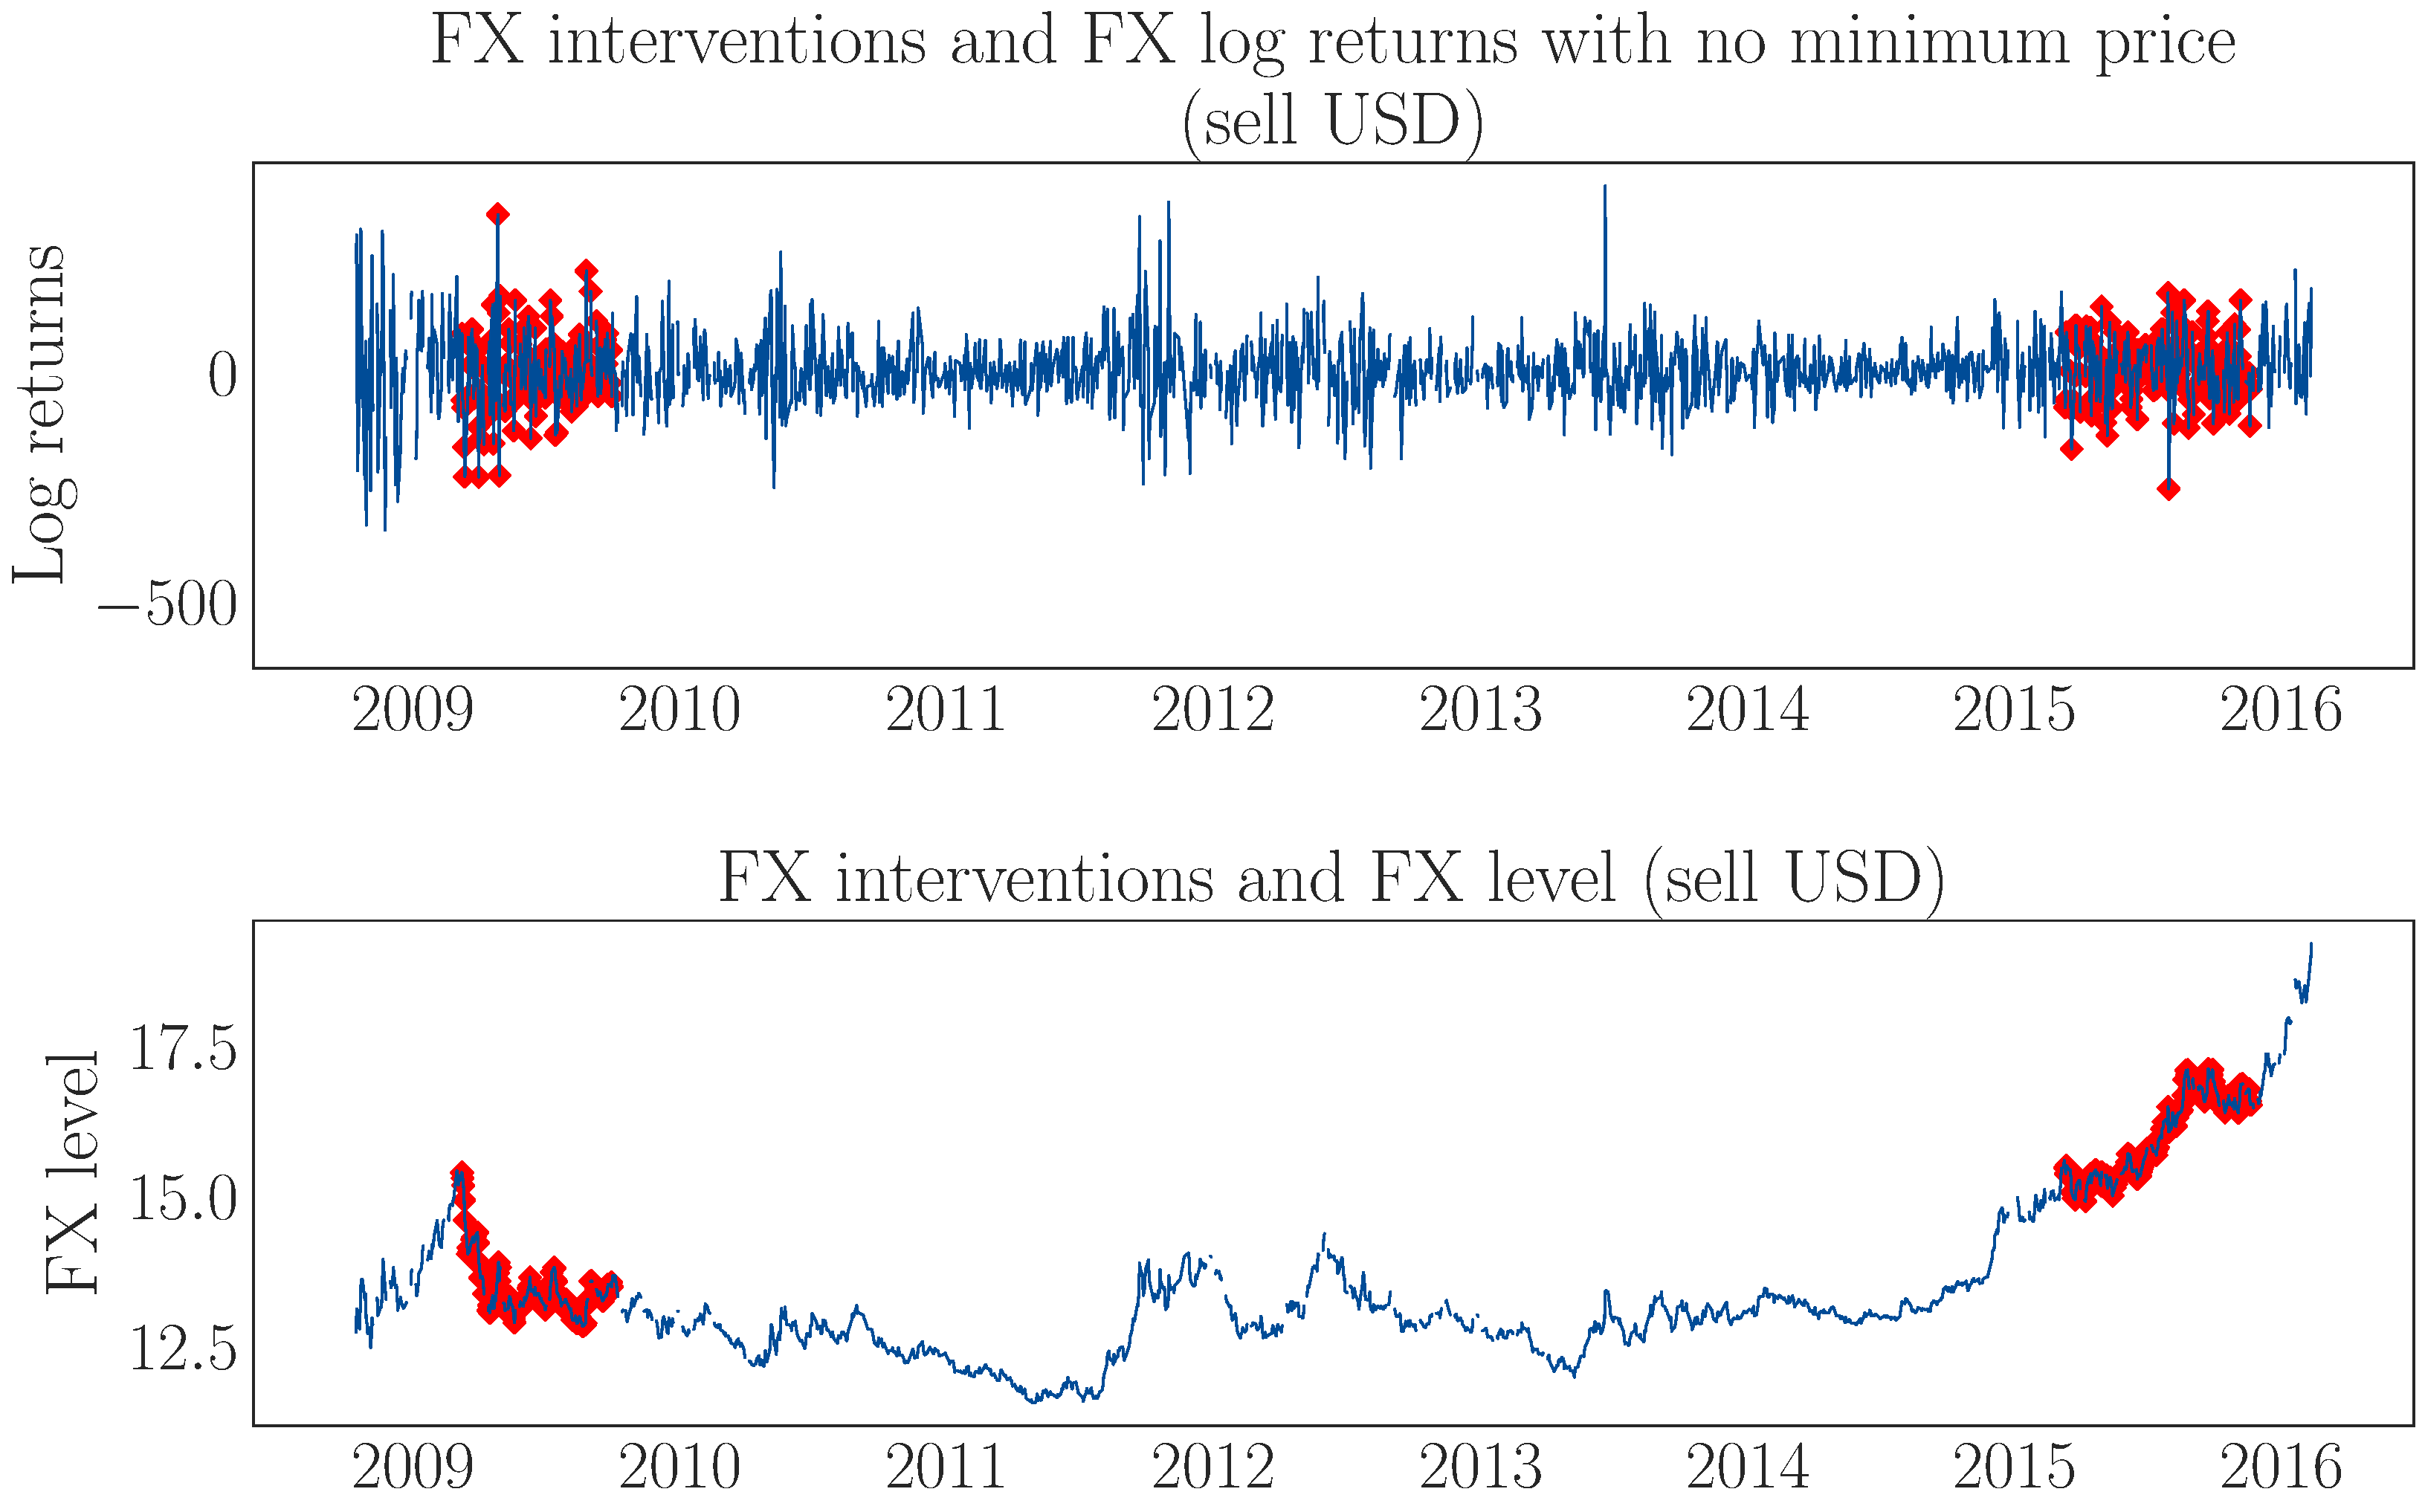
\includegraphics[width=                0.95\textwidth,
keepaspectratio]{../output/benchmark_no_minprice.pdf}
\label{fig:benchmark-nominprice}  \source{\emph{Sources}:   Banco  Mexico  and
authors' calculations}
\end{figure}


As in the case of interventions with  a minimum price, the conditional CDF can
be used to benchmark the FX interventions  relative to the risk of the day, as
presented  in Figure  \ref{fig:benchmark-nominprice-cdf}. While  interventions
with  a  minimum price  exhibited  a  pattern  broadly consistent  with  large
depreciation  pressures on  the  exchange rate,  the  interventions without  a
minimum price  have no clear  risk patterns.  Such interventions  had occurred
across the full conditional distribution, even  when the pressures were not on
the depreciation  side but, on the  contrary, the appreciation side.   In this
case, the  fact that the central  bank was selling USD  could have, therefore,
amplified the currency appreciation.  This pattern likely suggests that the BM
rationales for  FX intervention  under the  no minimum  price rule  are likely
broader than  just the volatility of  the exchange rate.  For  example, during
certain periods, the motivation for  interventions without a minimum price was
to prevent excessive  accumulation of foreign reserves,  explaining that those
interventions were not related to FX rate developments.\\

\begin{figure} \centering
  \caption{FX Interventions  without a  Minimum Price  on the  Mexican Peso/US
Dollar}                 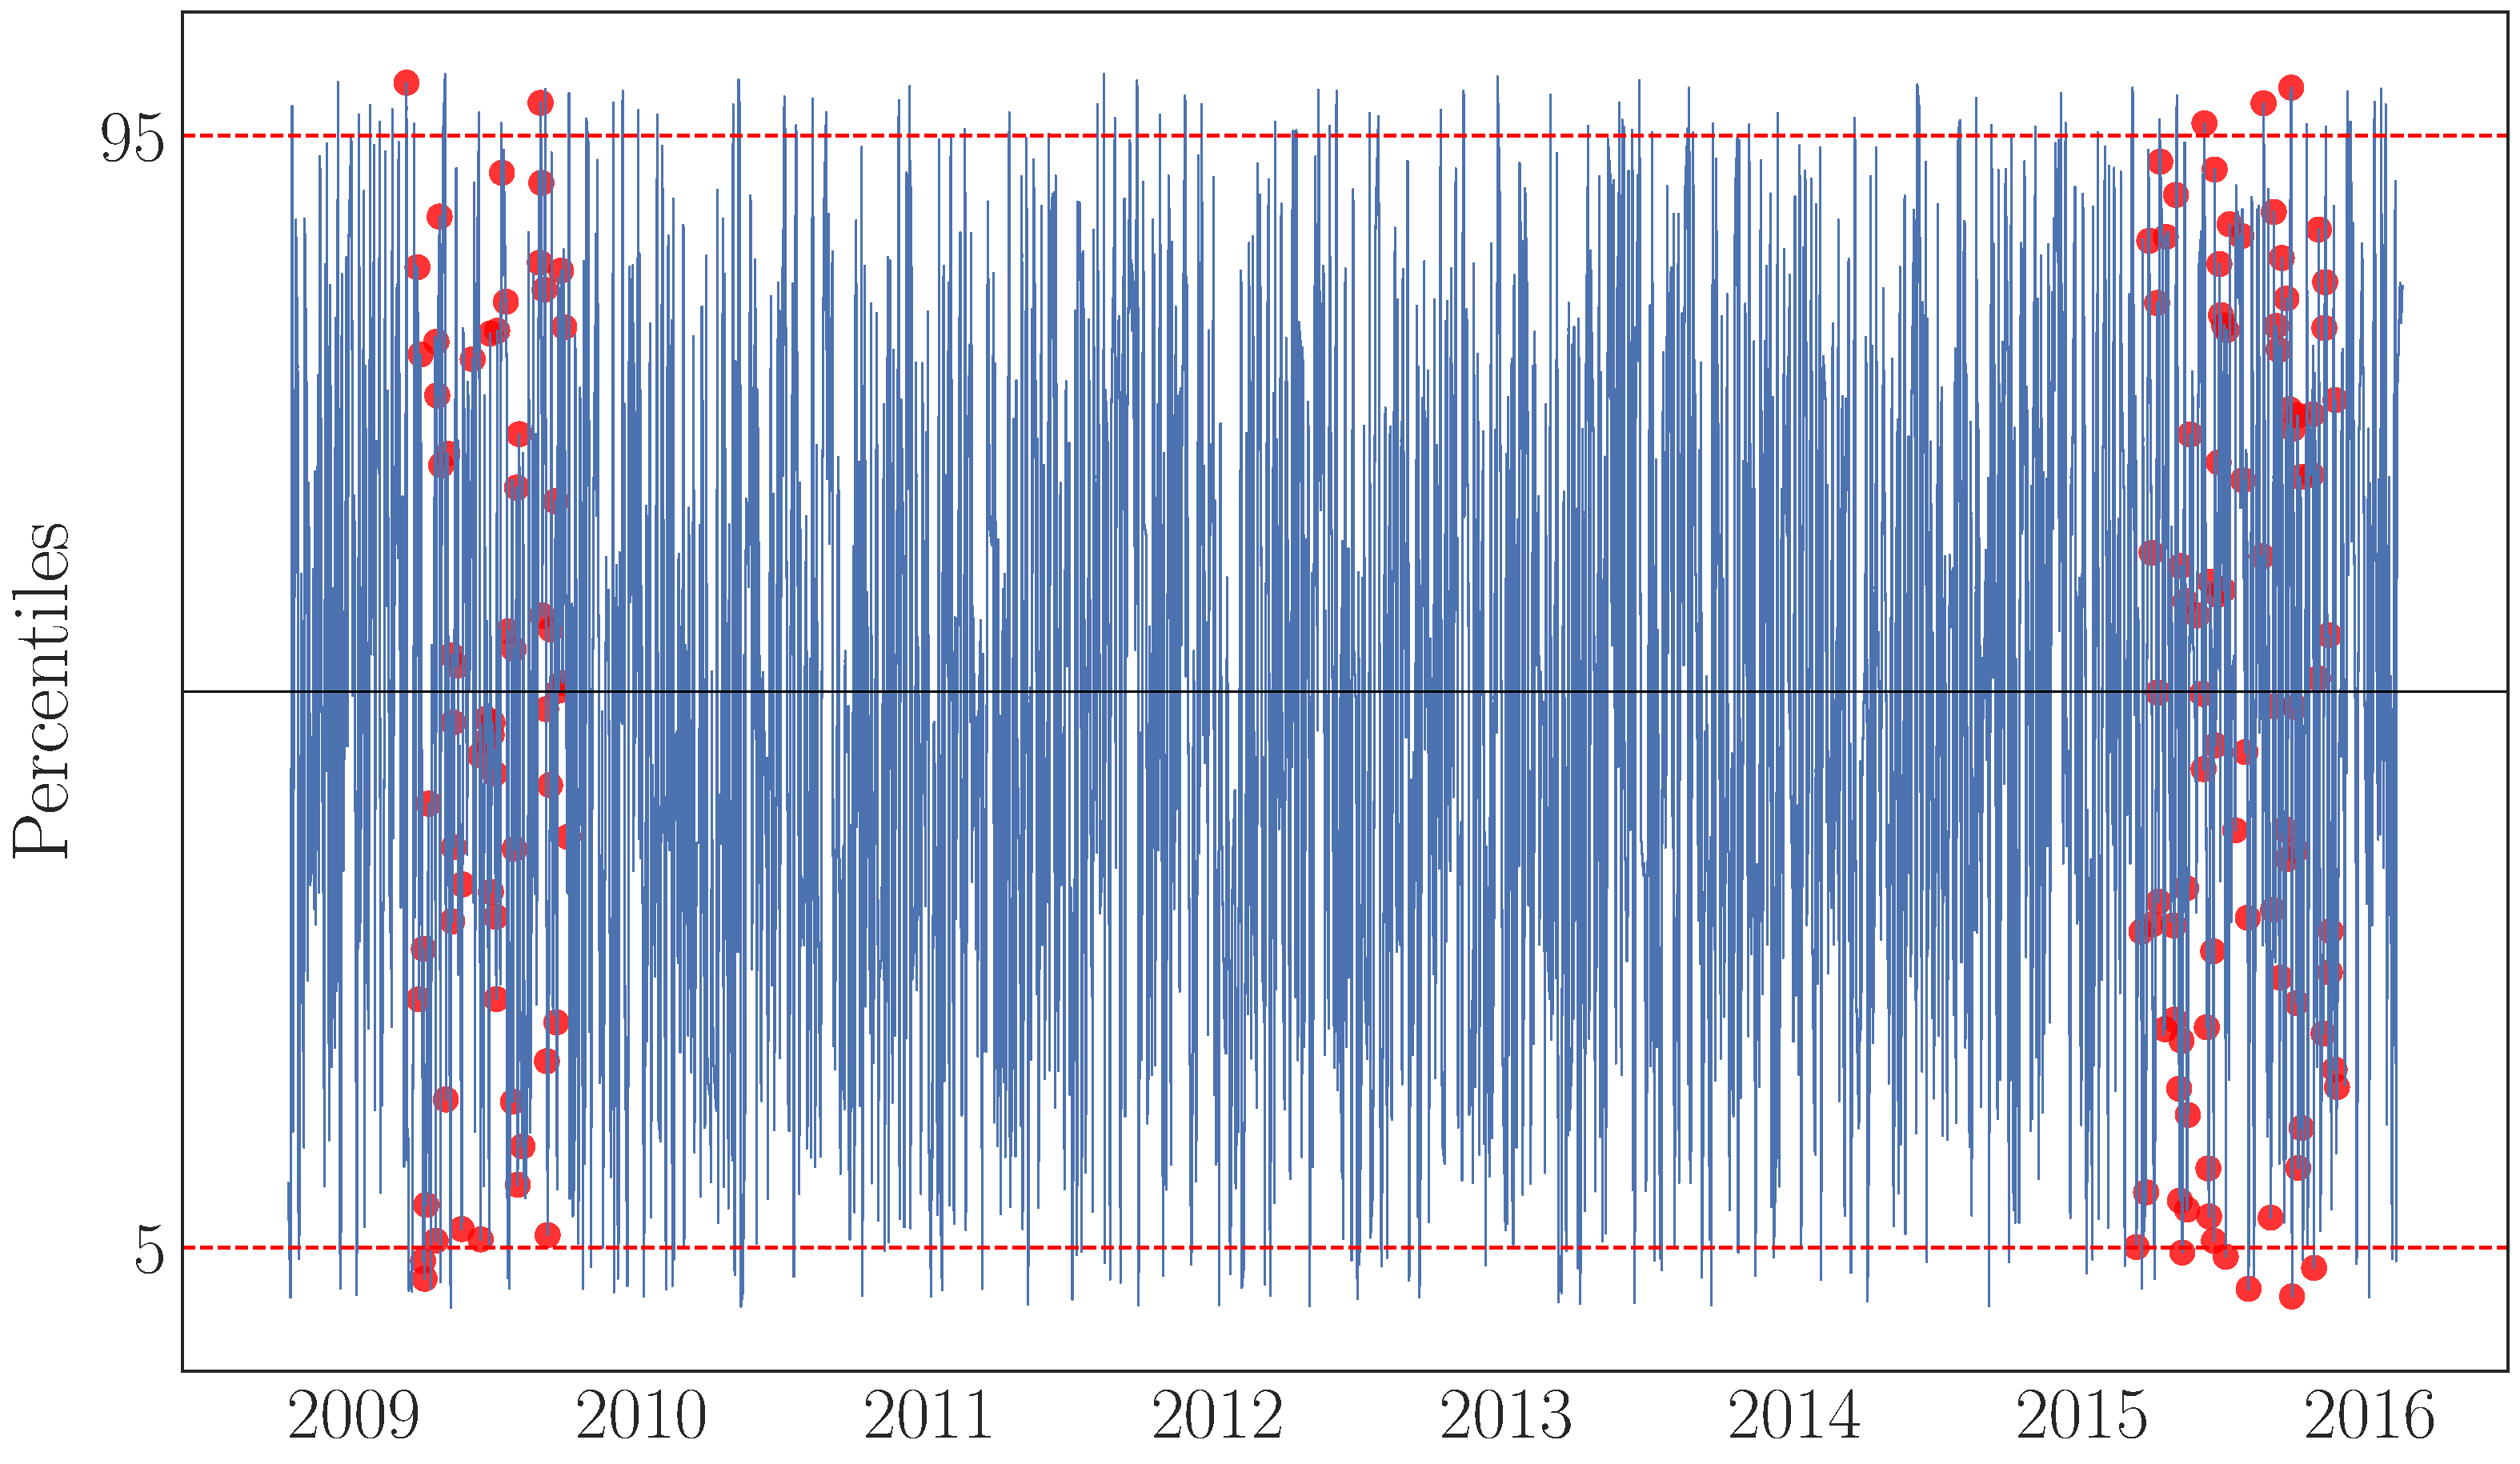
\includegraphics[width=                0.95\textwidth,
keepaspectratio]{../output/benchmark_no_minprice_cdf.pdf}
\label{fig:benchmark-nominprice-cdf} \source{\emph{Sources}:  Banco Mexico and
authors' calculations}
\end{figure}

%% ---------------------------------------------------------------------------
%% Conclusion %%
%% -----------------------------------------------------------------------------

\section{Conclusion}
\label{sec:conclusion}

Foreign   exchange    interventions   would   benefit   from    a   risk-based
framework. Central  banks use quantitative  tools such  as VaR to  measure the
risk  on their  foreign  reserves  portfolio or  when  they  accept assets  as
collateral for their  loans. In this paper, we argue  that central banks could
also use this  concept when they intervene  to support the FX  market, as FXIs
often aim at removing some exchange rate risk from the market.\\

The model  of this paper has  several policy implications. The  VaR rule would
help central banks  concerned about financial stability risk  arising from the
exchange rate but  committed to a floating exchange  rate arrangement. Central
banks  could  accompany  the  transition   to  exchange  rate  flexibility  by
formalizing the commitment to the float  in a rule and by gradually increasing
the VaR;  i.e., reducing  intervention frequency, to  allow for  more exchange
rate volatility. Finally, the VaR rule could be used to deepen hedging markets
by gradually transferring an increasing share of the exchange rate risk to the
market.\\

A risk-based  approach has  convincing advantages relative  to other  types of
rules. Compared with  fixed-volatility rules, the VaR rule  allows the central
bank  to control  exactly  the exchange  rate  risk to  which  the economy  is
exposed. It  also facilitates preparing  the intervention budget based  on (i)
the fixed FXI frequency; (ii) the maximum FXI amount; and (iii) the FX reserve
adequacy constraint.  Other  advantages include being budget  neutral over the
medium  term,  forward looking,  and  combining  several exogenous  variables,
reflecting  both competitive  shocks and  market structure  factors, into  one
trigger.\\

While it  does not  allow to  identify the nature  of the  shocks, such  as to
guaranty the optimality  of each FXI, the  VaR rule is flexible  enough to let
the exchange rate timely adjust to  new equilibria. It also allows the central
bank  to  respond to  market  disfunctions  reflected  in high  exchange  rate
volatility and contributes to prevent exchange rate overshot. Finally, the VaR
rule is easier to implement and  operationalize in markets at different stages
of development than rules that would try determining the nature of shocks.\\

The  paper  argues  that  using  VaR   as  an  input  would  contribute  to  a
better-informed FXI policy decision.  It would  help to anchor the decision to
intervene on the risk hedging objective  of the policymaker and the structural
weaknesses  of  the economy,  such  as  unhedged  exposures to  exchange  rate
risk. In  summary, the  VaR rule,  while not currently  widely used,  could be
considered  as  one approach  to  build  a  solid and  consistent  operational
framework for FXIs.\\

Looking beyond interventions in the spot FX market, similar models and methods
can be  used by  central banks to  transfer risk from  any markets  to support
financial stability.  Considering  the focus on UIP deviation in  the IMF IPF,
the VaR rule can be amended to target tail UIP deviations instead of tail spot
volatility.   The VaR  would be  a natural  benchmark to  determine how  large
deviations  would signal  market  impairment. Benchmarking  the deviations  is
important as forward  rates deviate from the  UIP most of the  times and those
deviations can be volatile, so there is  a need to define a reasonable anchor,
so that the frequency of central  bank interventions is adequate. Moving on to
the hedging market, the VaR rule can  also be used to identify unusually large
increases in the cost of hedging  that could reflect hedging market impairment
and spill over to  the spot market. In that case,  the relevant variable would
be the  spread between forward  rates and  the covered interest  parity, which
reflects   the   cost   of  hedging   (\cite{borio2016},   \cite{cerutti2019},
\cite{du2018}, and \cite{eguren2018}).\\

One issue that remains to be addressed  is how to determine the optimal degree
of hedging provided by the central bank  to the market and what should be left
in the  market. The  paper discussed the  structural factors  underpinning the
underlying risk  to be covered  in broad terms,  that is, direct  and indirect
exposures  to  exchange rate  risk.   However,  it is,  so  far,  left to  the
policymakers'  judgment to  translate those  vulnerabilities into  an optional
level of  hedging to be  offered by  the central bank;  i.e., a target  VaR. A
method that estimates the extent of the vulnerabilities and combined them with
their impacts  on macro-financial  stability is left  for future  research and
would be most useful.\\



%% ---------------------------------------------------------------------------
%% Bibliography
%% ---------------------------------------------------------------------------
\newpage
\addcontentsline{toc}{section}{References}
\singlespacing
\bibliographystyle{apalike2}
\bibliography{bibliography}

%% ---------------------------------------------------------------------------
%% Annex I
%% ---------------------------------------------------------------------------
\newpage
\appendix 
\section{Comparative Static Financial Performances}
\label{sec:fin-perf}

This  appendix  presents a  comparative  static  evaluation of  the  financial
performance of  the three  different intervention  strategies studied  in this
paper: the strategy without a minimum price, the strategy with a minimum price
(rule-based), and  the VaR  rule strategy.  We selected  a one-year  period of
intervention,  between  October  2015  and  October  2016.  The  frequency  of
intervention  under the  no minimum  price  and the  minimum price  strategies
during this  time was the same  (18 interventions each), with  similar volumes
(USD 3.32 billion  and USD 3.6 billion, respectively). Then,  we constructed a
series of  interventions following  the VaR  rule at  a similar  frequency (18
interventions), corresponding to a 10  percent intervention threshold, only on
the selling side to match the other strategies. We calibrated the intervention
amount  of the  VaR rule  to be  at  the average  under the  no minimum  price
strategy so that  the total amount of intervention under  the VaR rule exactly
matched the intervention amount under the no minimum price strategy.\\

This financial benchmarking is purely a comparative exercise. It might be that
some interventions without  a minimum price complemented  interventions with a
minimum price  and were executed at  a less favorable time.  The comparison is
not taking such a selection effect  into account and should not be interpreted
as  definite  proof of  the  financial  performance  of one  strategy  against
another.  Under  this  caveat,  the benchmarking  shows  that  the  rule-based
strategies (either  minimum price or  VaR based) outperform the  minimum price
strategy, as presented in the table below.\\

Table \ref{tab:financial-perf} reports  that on average, under  the no minimum
price  rule, the  central bank  was selling  USD when  the local  currency was
slightly appreciating against  the USD (by -6 bps; the  negative value in this
quotation  means appreciation).   Under the  minimum  price and  the VaR  rule
schemes,  on the  contrary, the  central bank  was selling  USD during  a more
favorable time.  By design, the VaR  rule is selecting days  with particularly
large depreciation, in  the order of 160 bps. Likewise,  the minimum price and
VaR rule scheme were  executed at much better rates in  terms of level.  While
the VaR rule  is designed to target the tails  of the conditional distribution
of the  log returns, it does  not necessarily guarantee that  the intervention
will happen  at the most favorable  exchange rate level. Our  simulation shows
that on average, it does nevertheless trigger interventions under better terms
than for the two other schemes.\\

Looking  at the  performance against  the  strategy without  a minimum  price,
computed against  the gain realized by  selling on average the  same volume of
USD at different points in time,  the benchmarking exercise indicates that the
minimum price  intervention would  outperform the  strategy without  a minimum
price by 7 percent, while the VaR rule would outperform it by 8.3 percent.\\

\begin{table}
  \begin{center}
    \caption{Financial Performances with and without Minimum Price}
%\footnotesize  %%  command to change the font size
\begin{tabular}{llll}
\toprule
{} & No minimum price & Minimum price & VaR rule \\
\midrule
Daily variation bps                  &             -6.1 &         108.8 &    164.8 \\
Average exchange rate                &             16.6 &          17.8 &       18 \\
FX Performance against discretionary &              0 \% &         6.9 \% &    8.3 \% \\
Total volume bn USD                  &             3.32 &           3.6 &     3.32 \\
Number of interventions              &               18 &            18 &       18 \\
\bottomrule
\end{tabular}

%\normalsize
\source{\emph{Sources}: authors’ calculations}
\label{tab:financial-perf}
\end{center}
\end{table}

\clearpage

%% ---------------------------------------------------------------------------
%% Annex II
%% ---------------------------------------------------------------------------
\section{Out-of-Sample Benchmarking}
\label{sec:benchmarking}

This  appendix  presents  a  series  of alternative  models  to  estimate  the
conditional density of  foreign exchange log returns over  time.  Our baseline
model  relies on  an EGARCH(1,1)  with a  Tskew parametrization  of the  error
terms’ distribution.   The conditional benchmark  models use the same  sets of
variables as our baseline model, presented in Section \ref{sec:specification},
and the same training/testing set.\\

We conduct benchmarking against:

\begin{itemize}
\item Different parametric variations of the GARCH model
  \begin{itemize}
  \item EGARCH(1,1) with Gaussian errors
  \item GARCH(1,1) with Tskew
  \item GARCH(1,1) with Gaussian errors
  \end{itemize}
\item Density estimation via quantile regressions. The full-fledged density is
  obtained via quantile interpolation and resampling, following the
  rearrangement procedure of \cite{chernozhukov2010}.
\item Unconditional distribution, estimated via Gaussian KDE on historical data
\end{itemize}

We assess  the performance metrics  of these models out-of-sample  against our
baseline model using (1)  PIT tests and (2) a density  log score, as explained
in \cite{diks2011}; we use the uncensored version of the log score.\\

We summarize  the results in  Table \ref{tab:benchmark-perf}. We  define "pass
the PIT  test" as: if  the estimated invert  CDF distribution lies  within the
uniform distribution  +/- 5 percent  interval confidence bands, as  defined in
\cite{rossi2019}, and "fail"  otherwise.  Regarding the density  log score, we
provide  both the  test statistic  (the average  difference of  the log  score
across  time)  and  the  p-value  of  the  test  statistic,  as  explained  in
\cite{diks2011}.   A   positive  test  statistic  indicates   that  the  model
outperforms the baseline  model, while the p-value tested  the null hypothesis
that the log scores of the two models are the same.\\

\begin{table}
  \begin{center}
    \caption{Results of the Out-of-Sample Benchmark Tests}
%\footnotesize  %%  command to change the font size
\begin{tabular}{lccc}
\toprule
  & PIT & Logscore diff against Baseline & Diff pvalue \\ 
  \midrule
	Baseline & Pass &  &  \\ 
	Unconditional & Fail & -6.36 & 0 \\ 
	Quantile Reg & Pass & -2.09 & 0.02 \\ 
	Gaussian EGARCH & Fail & 1.235 & 0.892 \\ 
	TSkew GARCH & Fail & 1.536 & 0.937 \\ 
  Gaussian GARCH & Fail & 1.86 & 0.968 \\ 
\bottomrule
\end{tabular}

%\normalsize
\source{\emph{Sources}: authors’ calculations}
\label{tab:benchmark-perf}
\end{center}
\end{table}

As Table \ref{tab:benchmark-perf} shows, the baseline model has a better log score than the
unconditional distribution and the daily distribution fitted from the quantile
regressions model  with resampling,  and these  two models  both fail  the PIT
test. However,  the difference against  variation of  the GARCH model  is less
clear cut:  while the  other models  outperform the baseline  in terms  of log
score,  the difference  is not  significant and  they also  fail the  PIT test
(albeit only  by a very  few numbers of  percentiles). Therefore, while  it is
clear that the GARCH specification is  appropriate to model FX returns―in line
with  the  literature―variations   around  the  type  of   GARCH  and  implied
distributions are statistically equivalent.\\

\begin{figure}
  \centering
  \caption{Unconditional Distribution PIT Test, Out-of-Sample}
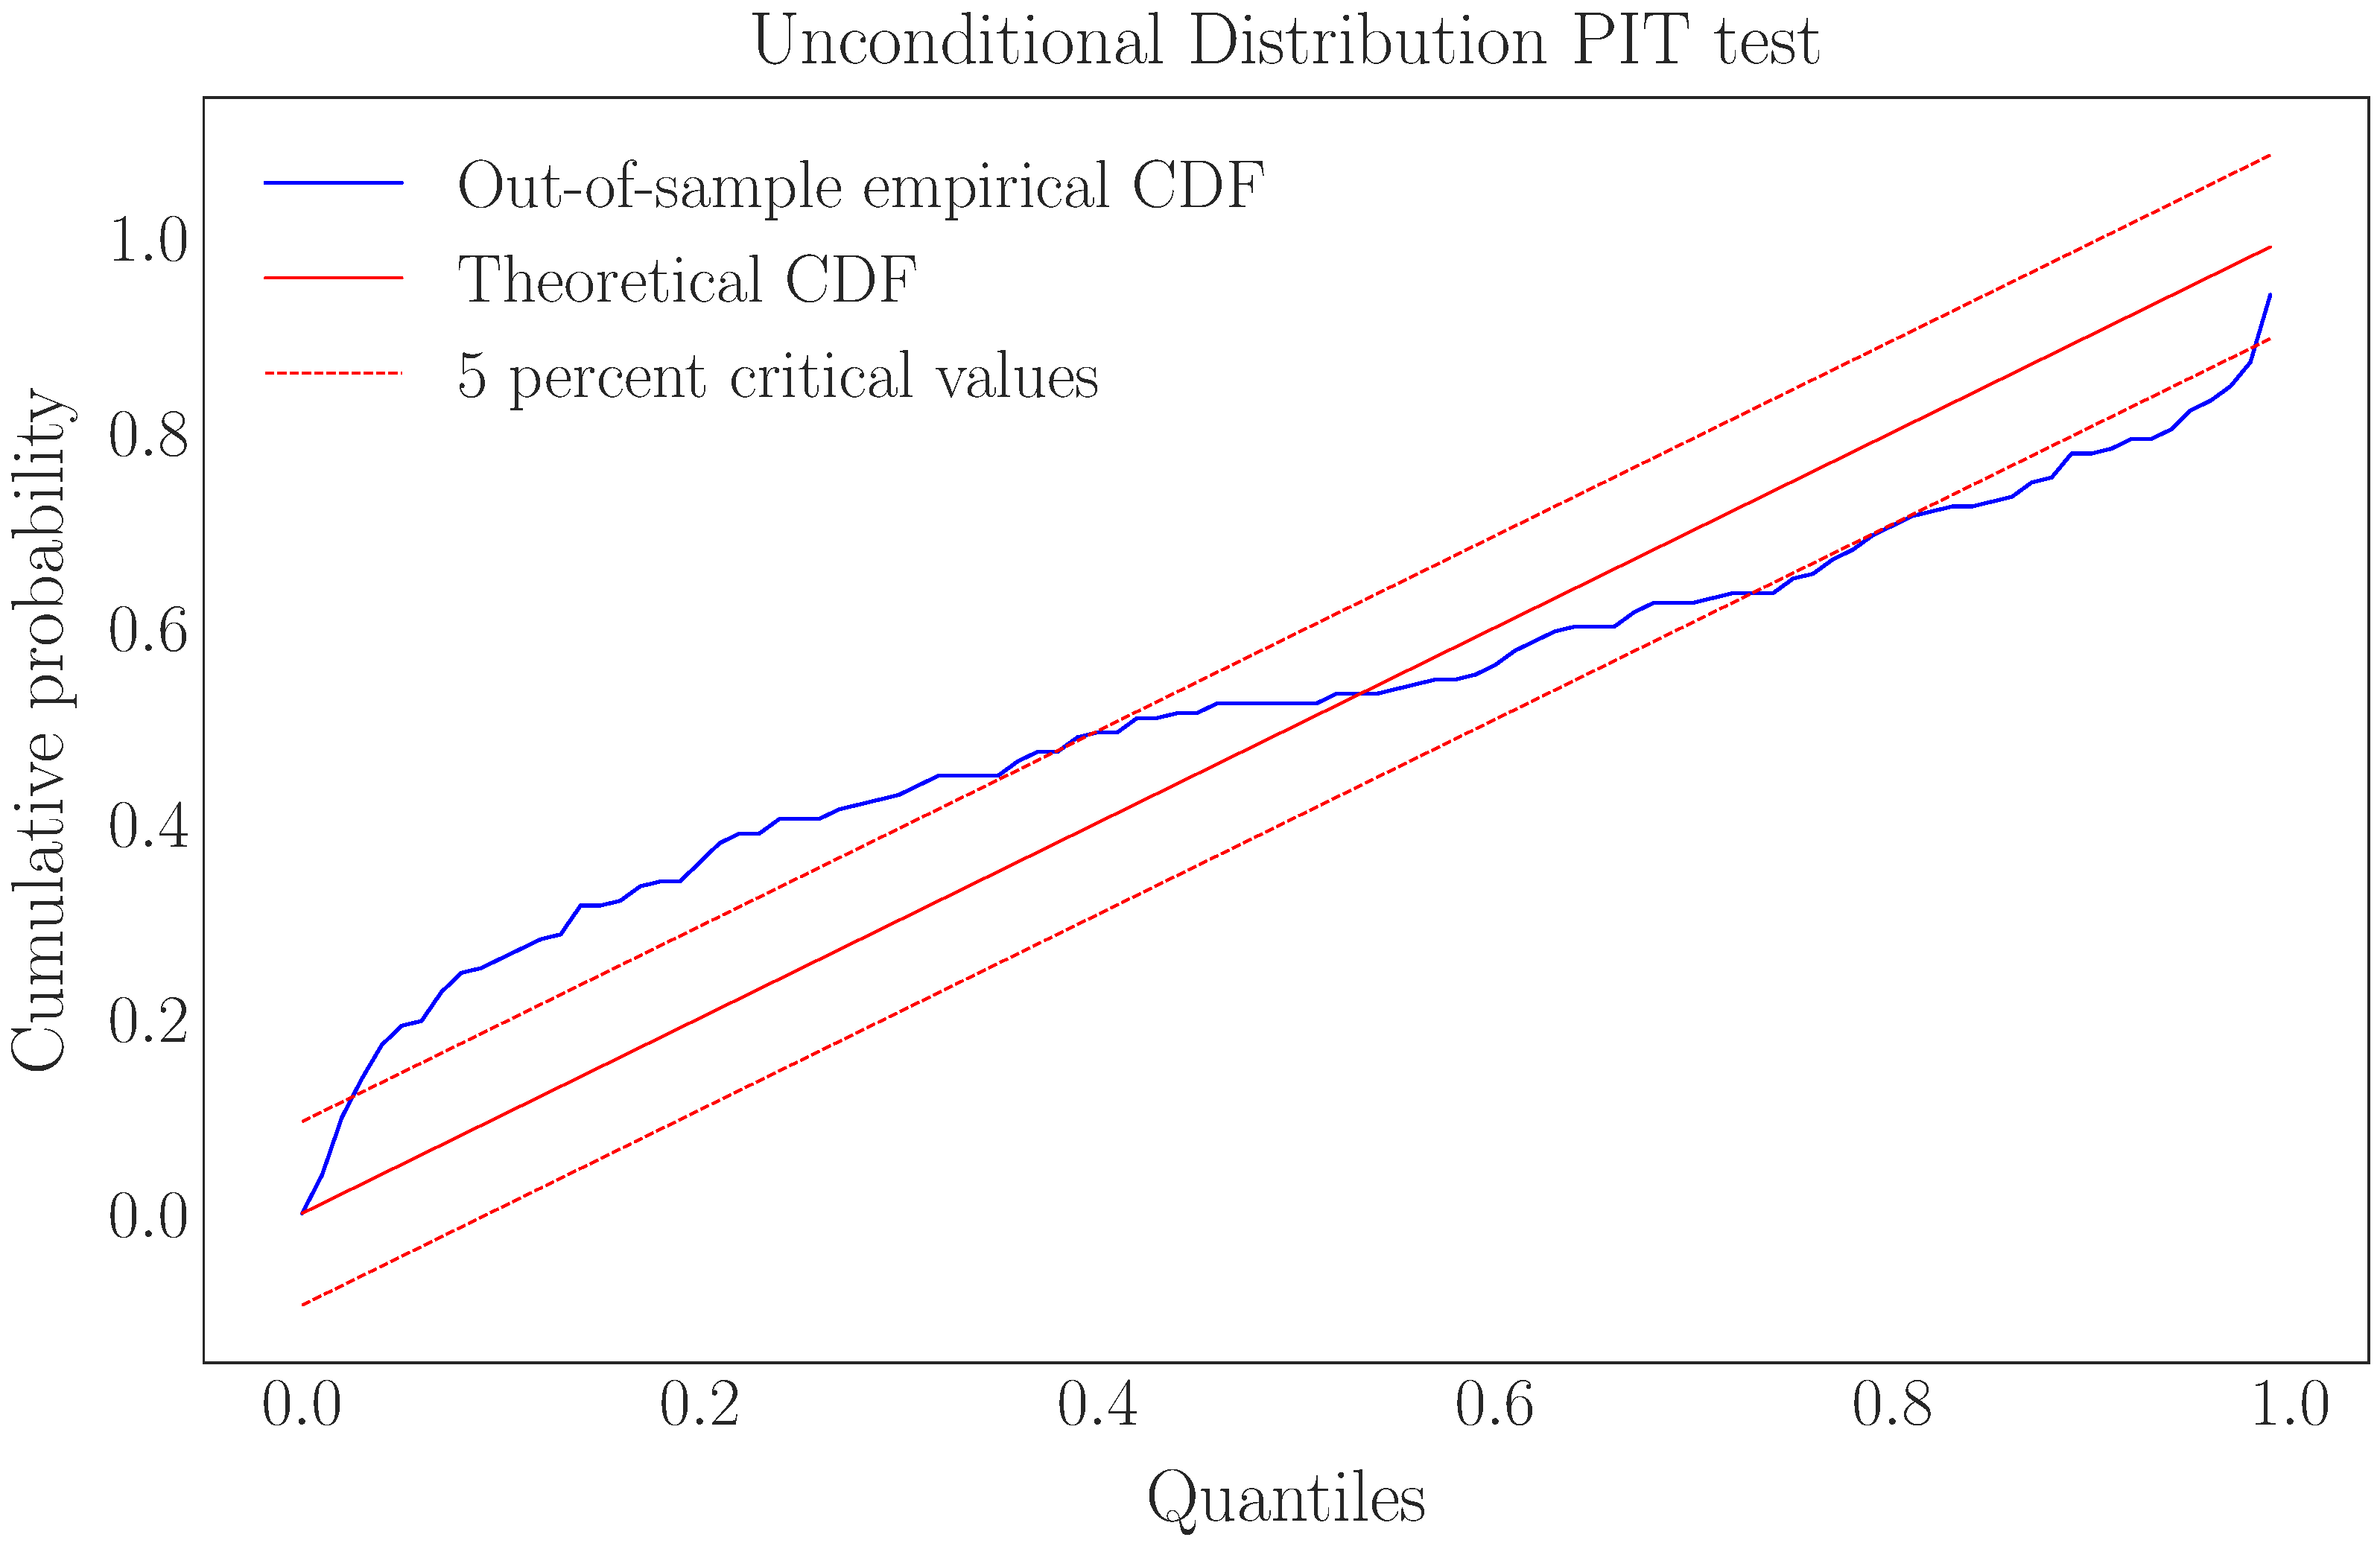
\includegraphics[width= 0.95\textwidth, keepaspectratio]{../output/pit_chart_unconditional.pdf}
\label{fig:pit-chart-unconditional}
\source{\emph{Sources}: authors' calculations}
\end{figure}

\begin{figure}
  \centering
  \caption{Quantile Regression Distribution PIT Test, Out-of-Sample}
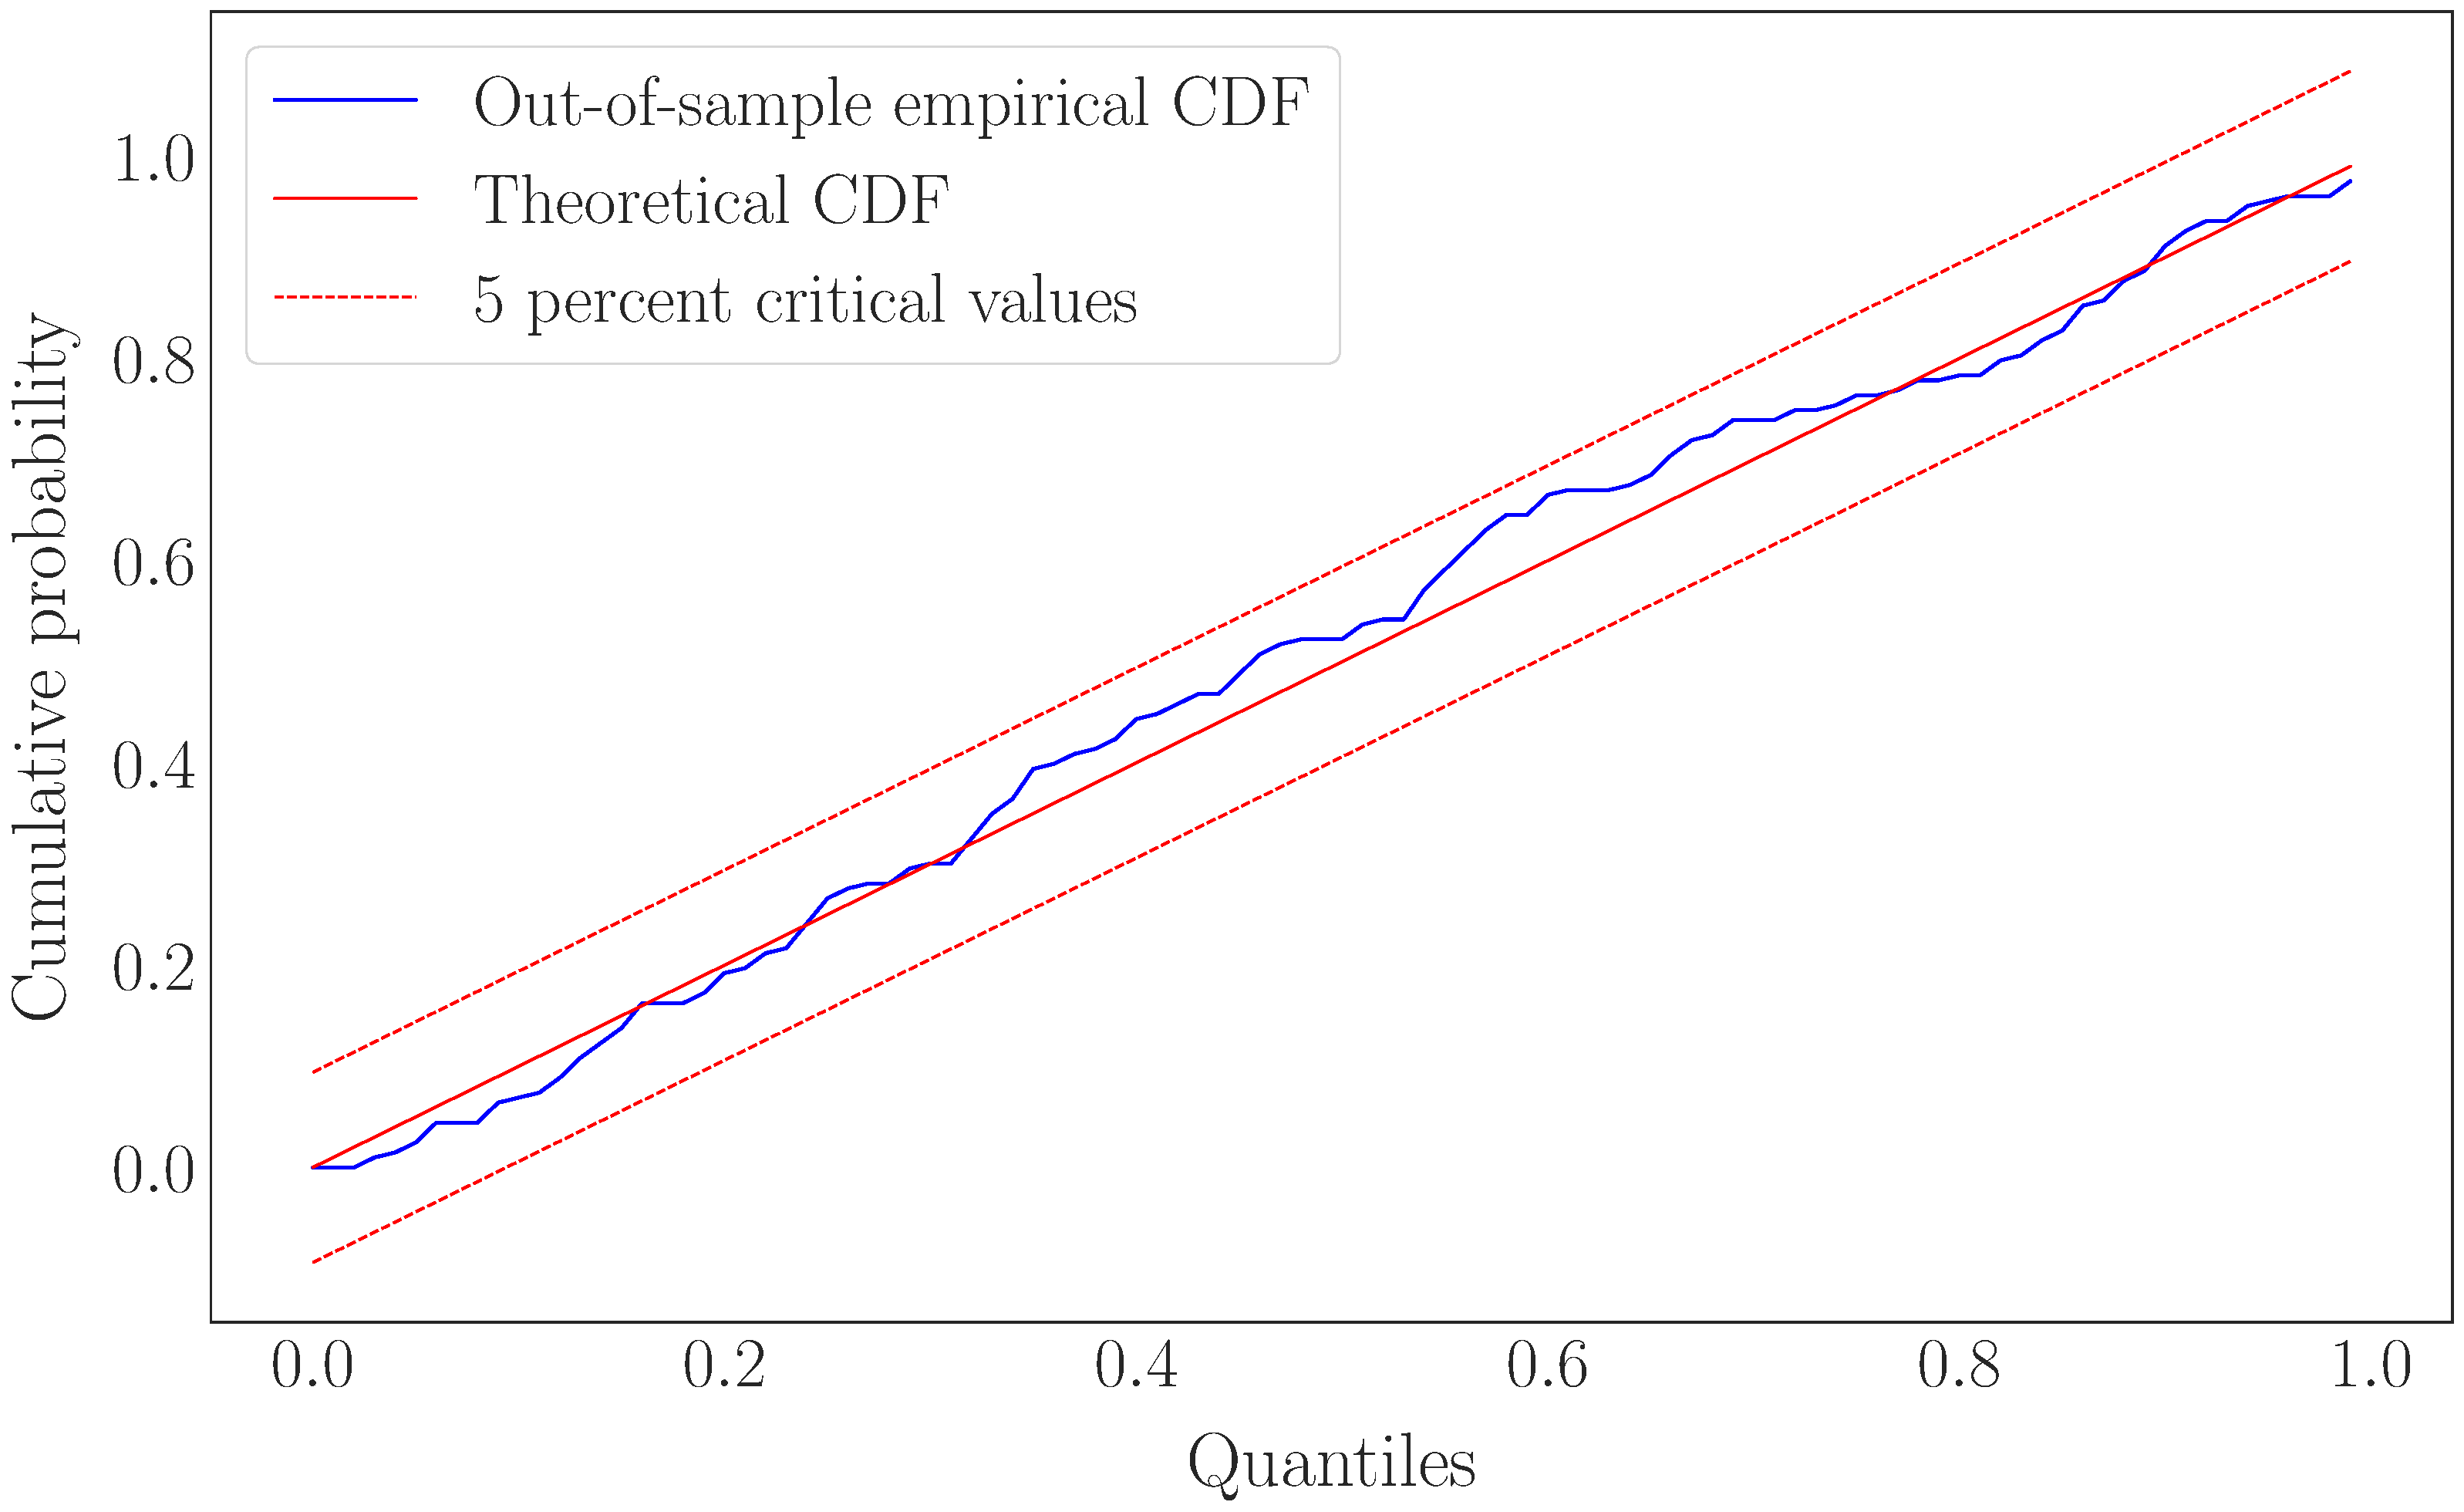
\includegraphics[width= 0.95\textwidth, keepaspectratio]{../output/pit_chart_qreg.pdf}
\label{fig:pit-chart-qreg}
\source{\emph{Sources}: authors' calculations}
\end{figure}


\begin{figure}
  \centering
  \caption{GARCH TSkew Benchmark PIT Test, Out-of-Sample}
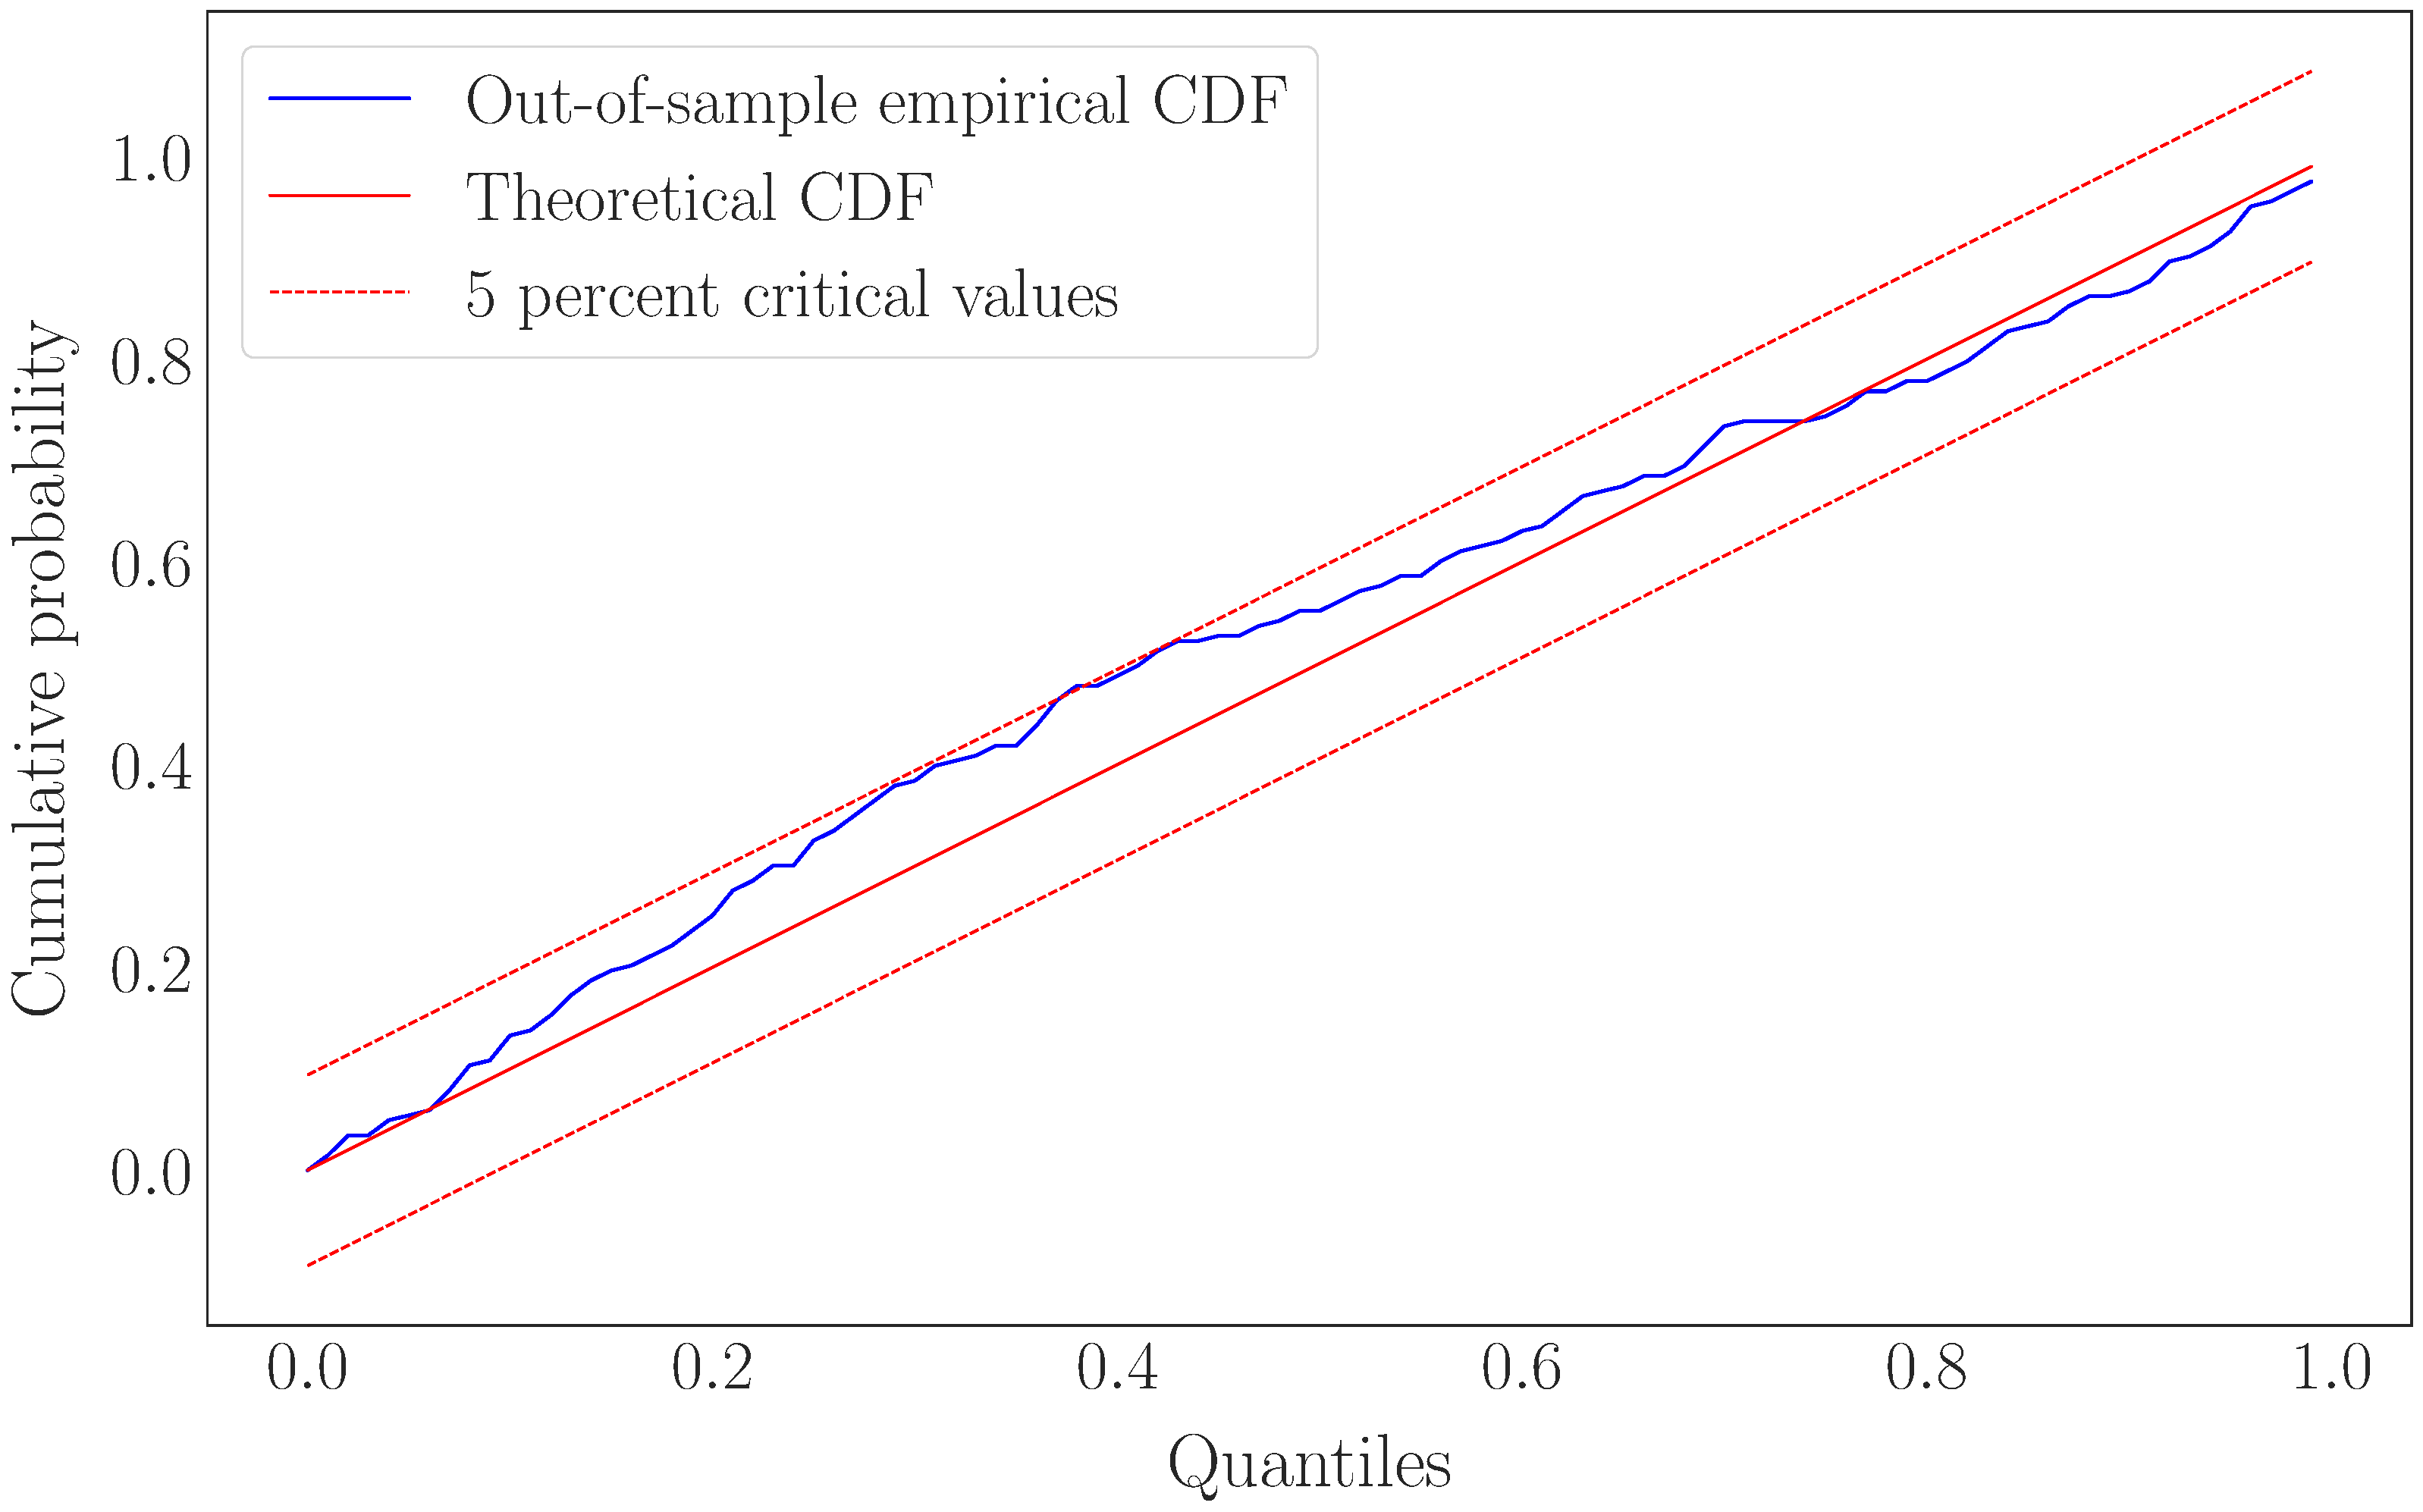
\includegraphics[width= 0.95\textwidth, keepaspectratio]{../output/pitchart_garch_tskew.pdf}
\label{fig:pit-chart-qreg}
\source{\emph{Sources}: authors' calculations}
\end{figure}







%% ---------------------------------------------------------------------------
%% End the document
%% ---------------------------------------------------------------------------
\end{document}
